\documentclass[]{zhawinesba} 

%\usepackage[final]{pdfpages}

%\graphicspath{{C:/Users/katrin/Documents/Dokumente/ZHAW/5Jahr/3_BA_documentation/ressources}}
\graphicspath{{../ressources}}

\title{Energy Harvesting Bicycle Computer}
%\subtitle{Bachelorarbeit Elektrotechnik}
\author{Katrin Bächli,\\Manuel König}
\tutor{Prof. Dr. Marcel Meli}
\cotutor{Herr Dario Dündar}

%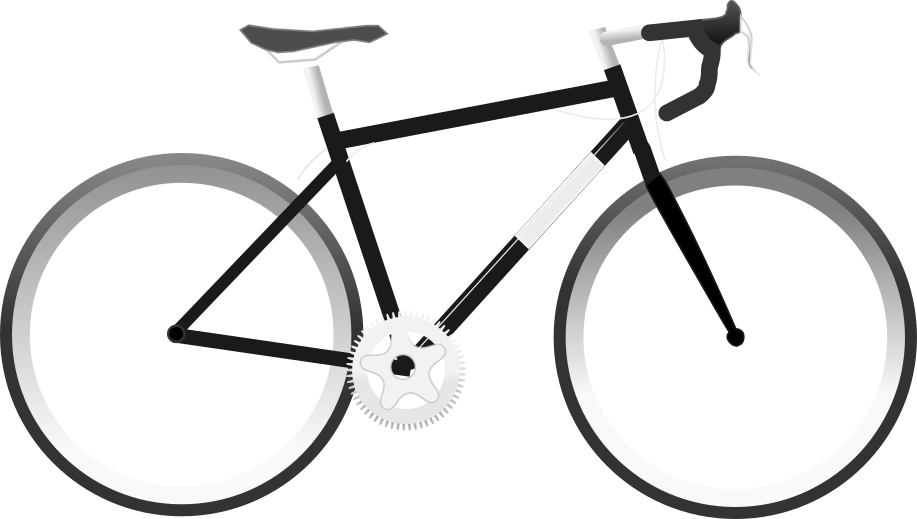
\includegraphics[scale=0.1]{0Titelblatt/road.png} 
\newcommand{\titleImagePath}{0Titelblatt/road.png}

%\makeatletter
%\let\oldpercent=\%
%\renewcommand{\%}{\ifmmode\oldpercent\else\thinspace\oldpercent\fi}
%\makeatother

\begin{document}


% hotfix for todos: 
% https://forum.finf.uni-hannover.de/index.php?page=Thread&threadID=10377
\setlength{\textwidth}{5.5in}    % temporär, original: 6.5in
%setlength{\evensidemargin}{1.1in} % temporär, original: 0.1in
\setlength{\marginparwidth}{3cm}  % for todos (so they don't get out of side}


\maketitle

\chapter*{Abstract}

The exchange of data between devices - commonly referred to as
\glqq Internet of things\grqq - should be made accessible to cyclists. The
mobile device should start to work at a cycling speed of 10km/h,
transmitting data through the Bluetooth Low Energy (BLE) protocol. The
task is based on a feasibility study which handles the energy
management through the chip EM8500. A \glqq SensorTag\grqq - available on Texas
Instruments Simple Link devices - is responsible for sending the data.
This board contains a wireless MCU and a low power Cortex M3.

The goal of the task was the development of a miniaturised board, which
should not be bigger than the utilized TI-SensorTag while adjusting the
energy storage, energy management and the power consumption of the
code. The finished product contains the hardware and a user friendly
Android application. The \glqq app\grqq allows adjusting the sensor readouts and
displays a tachometer and a speedometer showing the current speed, which is based on the radius of the wheel).

At the start, a feasibility study was conducted. The feasibility study
version showed promise for enough energy being produced at speeds
over 45km/h.

After improving the energy harvest we were able to generate 20
$\mu$W at 10km/h. The energy management of the EM8500-Chip and the
firmware of the TI-SensorTag were then completely rewritten. The
threshold of the energy management is based on the MPP of the harvester
and the goal is to send constant BLE-data at 10km/h. The firmware of
the TI-SensorTag uses sleep functions to reduce the energy
requirements.

The prototype is a configurable BLE-application, which sends speed,
pressure, temperature and air moisture data in 1.5 minute intervals at
10km/h. From 20km/h onward, the data is sent every 20 seconds and over
45km/h the data is sent continuously.

\chapter*{Zusammenfassung}

Internet of Things, also die Möglichkeit, Daten unter Geräten auszutauschen, soll für einen Fahrradfahrer nutzbar gemacht werden. Das  mobile Gerät soll durch Energy Harvesting gespiesen werden und bei einer Geschwindigkeit von 10 km/h Sensordaten mit Bluetooth Low Energy (BLE) senden. Die Arbeit baut auf einer Machbarkeitsstudie auf, die das Management der gewonnenen Energie mit dem Chip EM8500 löst. Als Sendemodul wird das SensorTag von Texas Instruments der Serie Simple Link benutzt. Dieses Board beinhaltet einen Wireless MCU und den Low Power Cortex M3. 

Aufgabe der Arbeit sind das Entwickeln einer minuaturisierten Leiterplatte, die nicht grösser als das verwendete TI-SensorTag ist, das Einstellen von Speicherelementen und von Schwellwerten für die Energiegewinnung und das Power optimieren des Codes. Als Produkt steht neben der Hardware eine benutzerfreundliche Android Applikation zur Verfügung. Diese beinhaltet Einstellungen der Sensoren und einen ansprechenden Tachometer, der die Fahrgeschwindigkeit anzeigt. 

Anfangs wird der Aufbau der Machbarkeitsstudie in Betrieb genommen. Die bestehende Version sendet Geschwindigkeit ab 45 km/h und basiert auf einem fliegenden Aufbau.
Nach der verbesserung der Harvesterschaltung, sodass bei 10 km/h rund 20 $\mu$W zur Verfügung stehen, wird der Print designt. Das Energiemanagment im EM8500-Chip und die Firmware des TI-SensorTags werden komplett neu geschrieben. Die Schwellwerte beim Energy Management basieren auf dem MPP des Harvesters und dem Ziel, konstant BLE-Daten bei 10 km/h zu senden. Bei der Firmware das TI-SensorTags werden über Sleep-Funktionen dem System genügend Zeit zum wieder Aufladen gegeben. 

Der Prototyp ist eine konfigurierbare BLE-Applikation, die bei 10 km/h jede 1.5 Minute Geschwindigkeits-, Druck-, Temperatur- und Luftfeuchtigkeitsdaten erhält. Bei 20 km/h werden die Daten nach 20 s und bei über 45 km/h konstant aktualisiert.

\chapter*{Vorwort}

Die Idee, Firm- und Software für einen Fahrrad-Computer zu schreiben, stammt vom Research-Assistenten vom InES, Herrn Dario Dündar. Die Themen vom Entwickeln einer Android-Applikation über das Schreiben einer Firm- und Software für einen Cortex M3 bis hin zum Layouten eines Prints sprachen uns, Manuel König und Katrin Bächli, sofort an. Ein Grund ist, dass das vorgeschlagene Projekt unsere unterschiedlichen Schwerpunkte, Manuel König wollte sich ins Schreiben einer Android-Applikation vertiefen und Katrin Bächli hat grosses Interesse an hardwarenahen Programmierung, bestens vereint.  

Manuel König erarbeitete bereits in seiner Projektarbeit eine Android-Applikation und wollte das Wissen vertiefen. Auch interessierte ihn, von Grund auf eine einfache Leiterplatte zu designen. Katrin Bächli hatte generelles Interesse an Energy Harvesting und fand die Idee, ihre C-Kenntnisse durch dieses Projekt zu vertiefen verlockend. Wir wussten, dass wir auf eine funktionstüchtige Erstversion eines Fahrrad-Computers zurückgreifen konnten. Dieser wurde in einer Projektarbeit entwickelte und dient als Starthilfe.

Während der Umsetzung des Prototypen verlagerte sich der Entwicklungsschwerpunkt zunehmend von der Software weg Richtung Hardware. Die Harvesterschaltung wird mehrfach optimiert, damit der Fahrrad-Computer schlussendlich bereits bei 10 km/h Daten an die Android-Applikation senden kann.

Bei der Entwicklung des Fahrrad-Computers wurden wir sehr gut betreut. In gemeinsamen, wöchentlichen Sitzungen nahm sich Prof. Dr. Marcel Meli und Research Assistent Dario Dündar Zeit. Sie setzten sich intensiv mit unseren Fragen auseinander und gaben sehr gute Vorschläge. Durch das Fachwissen konnten viele Fragen und Probleme gelöst werden. Wir lernten somit sehr viel durch dieses Bachelorarbeit. 

Wir möchten Dario Dündar und Marcel Meli an dieser Stelle nochmals explizit danken. Prof. Dr. Marcel Meli kennt das Konzept des verwendeten EM8500 sehr gut und half uns, die richtigen Korrekturen vorzunehmen. Besonders in der Hardware-Entwicklung stellte er wichtige Fragen, die uns halfen, noch bessere Lösungen zu finden. Die Unterstützung durch Dario war unglaublich. Das TI-SensorTag konnte falsch reagieren wie es wollte, er gibt nie auf und verhalf so, zu immer neuen Ansätzen und Lösungswegen. Ohne ihn würde der Fahrrad-Computer nicht bei 10 km/h fahren. Eine weitere wichtige Unterstützung erhielten wir durch Erich Ruff vom InES. Wir kamen beim Messen der Energie bei einer gewissen Geschwindigkeit an die Genauigkeitsgrenze. Er baute für uns einen Radimitator auf. So konnten wir genaue und reproduzierbare Messergebnisse erzielen. 

\begin{figure}[ht]
   
\includegraphics[width=0.25\textwidth]{0Vorspann/imag/delectric_logo_gross.png}
   %\caption{Delectric GmbH Logo}
   \label{delectric_logo} 
\end{figure}

Weiter danken wir Herrn Blum von Delectric GmbH, welcher uns die Leiterplatten für die Arbeit kostenlos und zeitnah zur Verfügung gestellt hat.

In dieser Projektarbeit konnte das ganze Wissen des Elektrotechnikstudiums angewendet werden: speziell vertieft worden sind die Themengebiete Elektrotechnik für die Bewegungsinduktion, Elektronik für die Schaltungoptimierung und das Leiterplatten-Design, die hardwarenahe Programmierung durch das Aufsetzen der Firmware und das Interrupt-Konzept. 


Winterthur, 10. Juni 2016


Katrin Bächli\\
Manuel König







\tableofcontents
\chapter{Einleitung}
In der heutigen Zeit gibt es viele interessante Gadgets, die unterschiedlichste Daten liefern. Seien das Pulsmesser, Heizungsregler oder das Multimediasystem zu Hause, diese Technologien lassen sich auch für den Fahrradfahrer nutzen. Es gibt bereits sogenannte Fahrradcomputer, welche die Geschwindigkeit messen und über ein separates Display ausgeben, jedoch werden die meisten mit einer Batterie betrieben, deren Laufzeit begrenzt ist. Mit der Möglichkeit des Energy Harvesting wird die Batterie und deren begrenzte Laufzeit gänzlich ersetzt. Bluetooth Low Energy kann Daten mit sehr wenig Energie übertragen, damit können die Daten, wie Geschwindigkeit oder Höhenmeter, an ein Android-Endgerät übermittelt werden.


\section{Ausgangslage}

Stand der Technik: Geschwindigkeitsanzeige für Velofahrer aktuelle Beispiele beschreiben.

Zwei Nachteile: Batteriewechsel und zusätzliches Display. Ein Handy hat jeder. Deshalb diese zur Anzeige benutzen.



Vorarbeiten auf diesem Gebiet:
Roman Scheider und Daniel Studer verfassten 2015 eine Projektarbeit am InES, in der sie die Machbarkeit eines Bicyle computer and sensoric powerd with energy nachwiesen \cite{PA_bicycle}. 
Die Punkte, die sich zu unser Arbeit unterscheiden benennen.

Nennen, was in dieser Arbeit \textbf{neu} erarbeitet wird.
...



\section{Definition der Aufgabenstellung}
Überleitung:Aufgrund STand der Technik, folgende Aufgabenstellung gebaut (Ist ev.Abschlusssatz Stand der Technik).

In der Ausschreibung der Arbeit ist der Inhalt der Bachelorarbeit zusammengefasst (siehe \ref{anhang_ausschreibung}). Das Ziel der Arbeit besteht darin, einen bestehenden Prototypen eines batterielosen Fahrradcomputers zu verbessern und zu optimieren. Die bestehende Hardware soll optimiert und bestenfalls verkleinert werden. Weiter soll eine App für ein Android-Endgerät entwickelt werden, in der die Messwerte dargestellt werden.

Aus den Themen entstand eine Aufgabenstellung mit folgenden Punkten:


% [label={\alph*)}]
\begin{enumerate} 

\item Inbetriebnahme des Prototypen, Einlesen in die vorangegangene Projektarbeit und Beschäftigung mit der Materie, sind die Hauptpunkte des ersten Schrittes.

\item Die bestehende Hardware muss verkleinert und überarbeitet werden. Dafür wird ein neues PCB entworfen, welches verschiedene vorhandene Platinen vereint.

\item Initialisierung der Bluetooth-Schnittstelle muss auf dem Android-Endgerät und der Hardware vorgenommen werden. Eine erste Bluetooth-Kommunikation zwischen der Hardware und der Applikationen ist implementiert.

\item Das bestehende Energiemanagement soll auf die Anwendung eines Fahrradcomputers optimiert werden.

\item Die Benutzeroberfläche der Android-Applikation soll benutzerfreundlich und optisch ansprechend gestaltet werden.

\item Die erfassten Messwerte der Geschwindigkeit und der aktuellen Höhe sollen über Bluetooth übermittelt werden.

\item	Die erfassten Daten sollen gespeichert und nur dann übertragen werden, wenn die nötige Energie vorhanden ist.

\item	Per GPS soll die aktuelle Position ermittelt, sowie die bereits abgefahrene Route erfasst werden. Alles soll auf einer Karte veranschaulicht werden.

\item	Die Beschleunigung, Luftfeuchtigkeit und Temperatur sollen ebenfalls erfasst und über Bluetooth übermittelt werden.


\item	Das Energiemanagement soll für verschiedene Geschwindigkeiten optimiert werden.
\end{enumerate}

Für diese Bachelorarbeit sind die Punkte a) bis f) als Minimalanforderungen zu verstehen, während sich die Punkte f) bis j) dynamisch und in Abhängigkeit des Projektfortschritts gestalten lassen.


Aus diesen Anforderungen entstand der im Anhang \ref{anhang_projektplan} abgelegte Projektplan. 






\section{Übersicht der Aufgabenblöcke}
Aus der Aufgabenstellung sind folgende Arbeitsblöcke (siehe Abbildung \ref{arbeitsbloecke} ) entstanden. Die gepunkteten Blöcke sind optional, die voll umrandeten das Minimum. Die Projektplanung ist so aufgebaut, dass bei Meilenstein 1, das Layout gezeichnet ist, bei Meilenstein 2 die Kommunikation zur App besteht, bei Meilenstein 3 die überarbeitete Version des Prototyps gezeigt wird und bis dahin das Minimum erreicht ist. Welche optionalen Ziele realisiert werden, wird im Meilenstein 3 definiert. Der Projektplan findet sich im Anhang \ref{anhang_projektplan}.

\begin{figure}[h]
    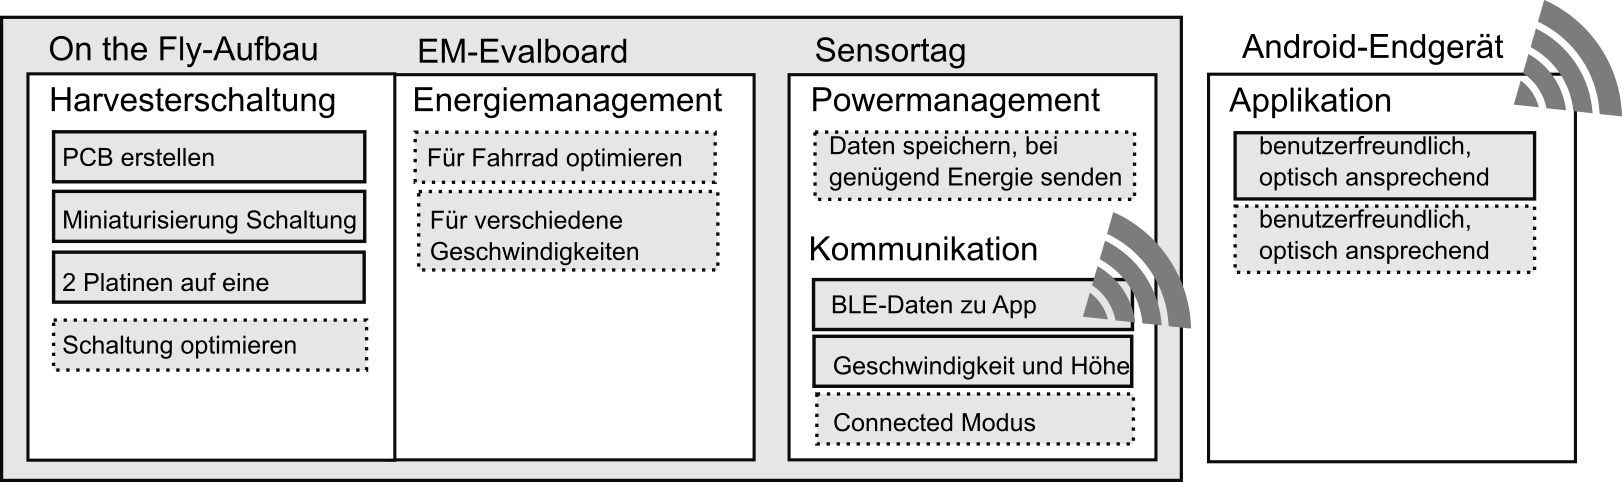
\includegraphics[scale=0.5]{../ressources/Projektorganisation/Arbeitsbloecke.png} 
    \caption{Arbeitsblöcke}
\end{figure}\label{arbeitsbloecke} 


\chapter{Theoretische Grundlagen}
Der Bicycle Computer basiert auf Energy Harvesting. Was Energie ernten bedeutet und welche Art von Energy Harvesting in dieser Arbeit angewandt wird, wird im ersten Unterkapitel \ref{t_harvesting} beschrieben. Im folgenden Unterkapitel \ref{t_energy_management} geht es um Ansätze zum Sammeln und Weiterleiten von Energie. Da die in Unterkapitel \ref{t_harvesting} gewonnene Energie im $\mu$W-Bereich liegt, ist zuerst ein Sammeln der Energie notwendig, sodass Leistungen im mW-Bereich zur Verfügung stehen. Das nächste Unterkapitel \ref{t_power_management} befasst sich mit dem notwendigen Power Management. Denn die
Energie soll nicht sofort verbraucht werden. Power Management regelt, wie schnell und wie viel Energie aufs Mal verbraucht werden soll. Als letzte Stufe in der Umsetzung ist eine energiearme Kommunikation notwendig. Da bietet die Bluetooth Low Energie Technologie ideale Voraussetzungen. Das Protokoll und die Technologie werden im letzten Grundlagenteil \ref{t_ble} vorgestellt.


% 2.1-------------------------------------------------------------------
\section{Energy Harvesting}\label{t_harvesting} 

\glqq Mit Energy Harvesting ... wird die Gewinnung von elektrischer Energie in kleinen Mengen aus dem Umfeld elektronischer Geräte für deren Betrieb bezeichnet.\grqq \cite{harvesting}. Als erstes werden Methoden zur Energiegewinnung vorgestellt (\ref{harv_arten}) und danach die im Bicycle Computer verwendete Harvesting Art genauer beschrieben (\ref{harv_bewegung}). Als letztes wird der Unterschied zwischen den Harvestingmethoden festgehalten. Denn diese Unterschiede werden in der Implementation des Bicycle Computers wichtig.


\subsection{Energy Harvesting Methoden}\label{harv_arten} 

Bekannte Methoden sind die Solarzelle, die aus der Energie der Sonnenstrahlen Strom erzeugt, die Thermogeneratoren (TEG), die aus Umgebungswärme Energie gewinnen,  passive RFID-Tags, die aus der elektromagnetischen Strahlung Energie gewinnen und der piezoelektrische Effekt, der mechanischen Druck in elektrische Spannung umwandelt. Da der im Prototyp verwendete Energy Mangement-Chip \cite{datasheet_EM85} für die Energieoptimierung von Solarzellen oder von Thermogenaratoren spezialisiert ist, werden diese zwei Methoden vorgestellt. 

\subsubsection{Energy Harvesting mit einer Solarzelle}\label{harv_solarzelle} 

Bei der Umwandlung von Elektromagnetischen Wellen (Licht) in Strom wird eine spezielle Eigenschaft des Siliziums genutzt: Führt man Silizium Energie zu, entstehen freie Ladungsträger, bzw. Elektronen und Löcher. Um aus diesen Ladungen einen elektrischen Strom zu erzeugen, ist es nötig, die erzeugten freien Ladungsträger in unterschiedliche Richtungen zu lenken; dies geschieht durch ein internes elektrisches Feld, welches durch einen p-n-Übergang erzeugt werden kann. Auf der einen Seite sammelt sich positive, auf der anderen Seite negative Ladung an. Werden diese verbunden, entsteht ein Strom (\cite{Internet_Solarzelle2}). 
Diese Harvestingmethode produziert ein Gleichstrom. Die Spannung am Ausgang ist konstant, da es sich um eine Stromquelle handelt \todo{stimmt das ?}. Grössen- und materialabhängig kann Energie im kW-Bereich gesammelt werden.

\subsubsection{Energy Harvesting mit einem TEG}\label{harv_TEG} 
TEG steht für Thermoelectric Generator und bezeichnet eine Konstruktion, die aus einem Temperaturunterschied elektrische Spannung erzeugt. Erzeugt wird die Spannung am Ende zweier metallischer Leiter aus unterschiedlichem Material, die an einem Ende verbunden sind (aus: \cite{Internet_Waerme}). Diese Harvestingmethode produziert eine Gleichspannung. Die produzierte Spannung ist vergleichsweise klein und bewegt sich im Bereich einiger 10 $\mu$V pro $1^\circ$C Temperaturdifferenz.


\subsection{Energy Harvesting über Bewegungsindktion}\label{harv_bewegung} 
Beim Bicycle Computer wird Energie über Bewegungsinduktion gewonnen. Die Funktionsweise ist in der Machbarkeitsstudie beschrieben \cite{PA_bicycle} S.8.:

Befindet sich eine Spule in einem \textit{dynamischen} \glqq Magnetfeld\grqq, wird in der Spule eine Spannung induziert. Dies sieht man in der Formel (\ref{Formel_induzSpannung}).

\begin{equation}
    U_{ind}=-\frac{d}{dt}\intop A\,dB \ \label{Formel_induzSpannung} 
\end{equation}

Der magnetische Fluss $B$ durch die Fläche einer Spule $A$ ist gleich dem magnetischen Fluss $\phi$. Hat die Spule mehrere Wicklungen $N$, so verstärkt sich der magnetische Fluss proportional. 

 
\begin{equation}
    \frac{d}{dt} \int A\,dB=\phi\cdot N\
\end{equation}

Verläuft der magnetische Fluss \todo{Flussdichte oder Fluss?} $\phi$ senkrecht zur Fläche der Spule $A$ kann das Integral durch eine Multiplikation ersetzt werden (siehe Formel\label{Formelsenkrecht}). 
 
\begin{equation}
    \frac{d}{dt} \int A\,\perp\, dB=\frac{d}{dt}\int \phi\cdot N=B\cdot A\cdot N\ \label{Formelsenkrecht} 
\end{equation} 
  
 
In diesem Fall berechnet sich die induzierte Spannung in einer Spule vereinfacht mit
\begin{equation}
    U_{ind}= - N \cdot A \cdot B
\end{equation}

Das dynamische Magnetfeld wird durch das Bewegen, oder im Fall eines Fahrrads einem Vorbeiziehen, eines Magneten an einer fix verankerten Spule erzeugt.
Die produzierte Spannung hängt von drei Kriterien ab:

Eine induzierte Spannung wird somit durch folgende vier Faktoren beinflusst:
\begin{enumerate}
    \item die eingeschlossene Fläche $A$ der Spule    
    \item die magnetische Flussdichte des Magneten $B$ 
    \item die Anzahl Windungen $N$ der Spule und
    \item die Bewegungsgeschwindigkeit $v$ des Magneten, welche Einfluss auf $dt$ hat
\end{enumerate}

Diese Harvestingmethode produziert einen Wechselstrom. Ein Gleichrichter und einen Kondensator zur Glättung der Rippelspannung ist nach der Energiegewinnung notwendig. Die Leistung der produzierten Spannung geht vom $\mu$W-Bereich bis zu für die Industrie optimierten Anlagen mit Leistung MW-Bereich wie z. B. durch Drehstrom-Generatoren.



\subsection{Unterschiede der Methoden}\label{harv_diff} 

Der grösste Unterschied besteht in der Art in der die Energie zur Verfügung steht. 

\subsubsection{Gleichmässige Energie versus gepulster Energie}
Die Solarzelle und ein TEG liefern Gleichstrom bzw. -spannung. Wodurch kein Gleichrichterschaltung und Glättung notwendig sind. Die durch Bewegungsinduktion gewonnene Energie ist eine Wechselspannung. Im Fall des Bicycle Computers ist diese gleichzeitig gepulst. Die Energie ist somit nicht konstant da, sondern nur in Zeitintervallen.

\subsubsection{Konstanter Maximum Power Point zu dynamischem}
Die drei Harvester unterscheiden sich in ihrer Leistungskurve. Das Leistungsmaximum, der Maximum Power Point (MPP), liegt auf der Skala von Kurzschluss bis Leerlauf proportional an unterschiedlichen Stellen.  Bei einem TEG liegt das MPP in der Mitte dieser Skala. Die MPPT-Ratio beträgt 50\thinspace\%. Bei der Solarzelle liegt das Leistungsmaximum auf der Skala bei ca. 80\thinspace\% der maximalen Spannung. Die MPPT-Ratio ist 80\thinspace\%.  Bei der Bewegungsinduktion existiert kein fixe MPPT-Ratio. Wie bei der Spule, wandert das Leistungsmaximum aufgrund mehrerer Indikatoren (wie Geschwindigkeit des Magneten durch die Spule, Abstand von Magnet und Spule) auf der Skala hin und her.

Zur Verdeutlichung der Unterschiede sind für jedes Leistungsverhalten eine Abbildung angefügt. Das TEG hat unabhängig von der gewonnenen Energie und der Temperatur das Leistungsmaximum immer bei 50\thinspace\%. Die Abbildung \ref{teg} zeigt, dieses unabhängige Verhalten. 

\begin{figure}[ht]
 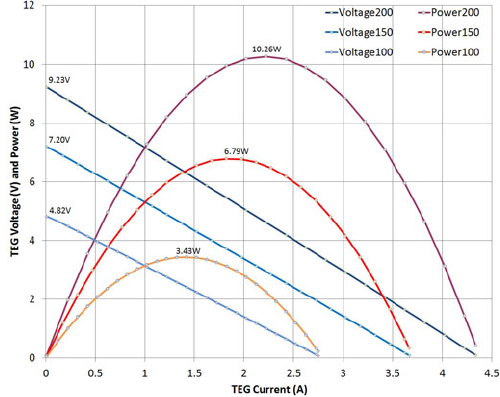
\includegraphics[width=0.5\textwidth]{2TheoretischeGrundlagen/imag/MPPTEG.png}
\caption{MPP TEG (\cite{MPP_TEG})}
\label{teg} 
\end{figure}


Abbildung \ref{mppsolar} zeigt, dass das Leistungsmaximum bei der Solarzelle unabhängig von der zur Verfügung stehenden Energie immer bei 80\thinspace\% liegt.

\begin{figure}[ht]
    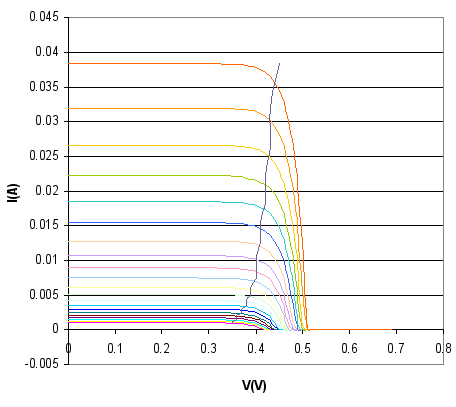
\includegraphics[width=0.5\textwidth]{2TheoretischeGrundlagen/imag/MPPSolar.png} 
    \caption{MPP Solarzelle (\cite{mpp_solar})}
    \label{mppsolar}
\end{figure}

Die Stelle des Leistungsmaximums wandert bei einer Spule und somit bei der Bewegungsinduktion auf der Skala. Exemplarisch sind drei MPPT-Ratios einer Spule in der Abbildung \ref{bildspule} abgebildet. In dieser Abbildung zeigt sich der Einfluss des Abstands der Spule vom Magnetfeld auf die Stelle der maximalen Leistung. Diese Abbildung wurde ausgewählt, weil beim Ausmessen des Harvesters der Abstand des Magneten als einer der Einflüsse festgestellt wurde. Im Kapitel \ref{ch_resultat} Resultat sind die ausgemessenen Leistungskurven des Prototypen in der Graphik \ref{mpp_resultat_harvester} abgebildet. Die Leistungskurven wurden für verschiedene Geschwindigkeiten aufgenommen und es zeit sich, dass bei der Harvesterschaltung analog zur Spule, die MPPT-Ratio wandert. Für den theoretischen Teil wurde die MPPT-Kurven des Harverster starkt geglättet und vereinfacht(siehe untenstehende Abbildung \ref{bild_harvester}). So ist der Effekt der Verschiebung des Leistungsmaximums besser ersichtlich wird. Es lässt sich grob über die MPPT-Ratio des Bicycle Computers sagen, dass sie sich zwischen 35 - 75\thinspace\% bewegt.

\begin{figure}[ht]
   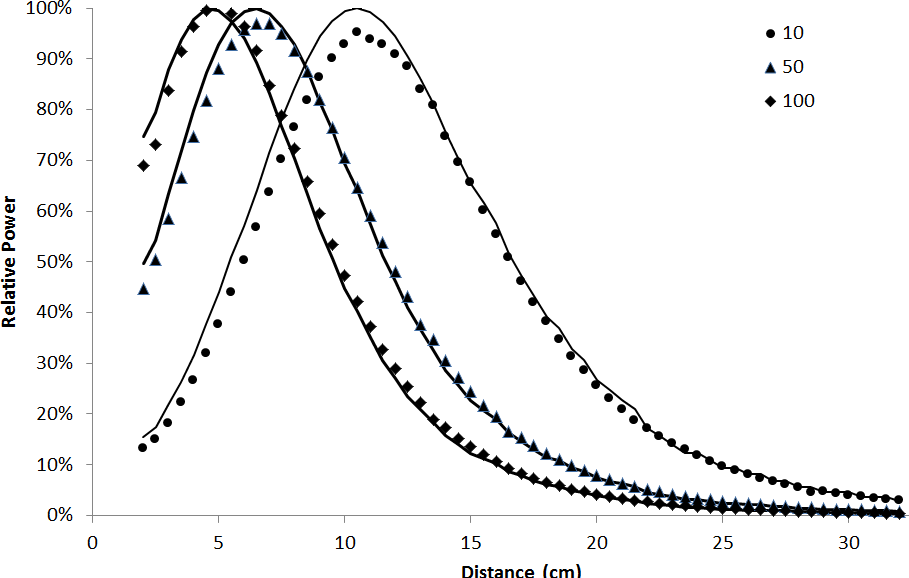
\includegraphics[width=0.5\textwidth]{2TheoretischeGrundlagen/imag/MPPSpule.png}
   \caption{MPP Spule (\cite{MPP_Spule})}
   \label{bildspule} 
\end{figure}

\begin{figure}[ht]
   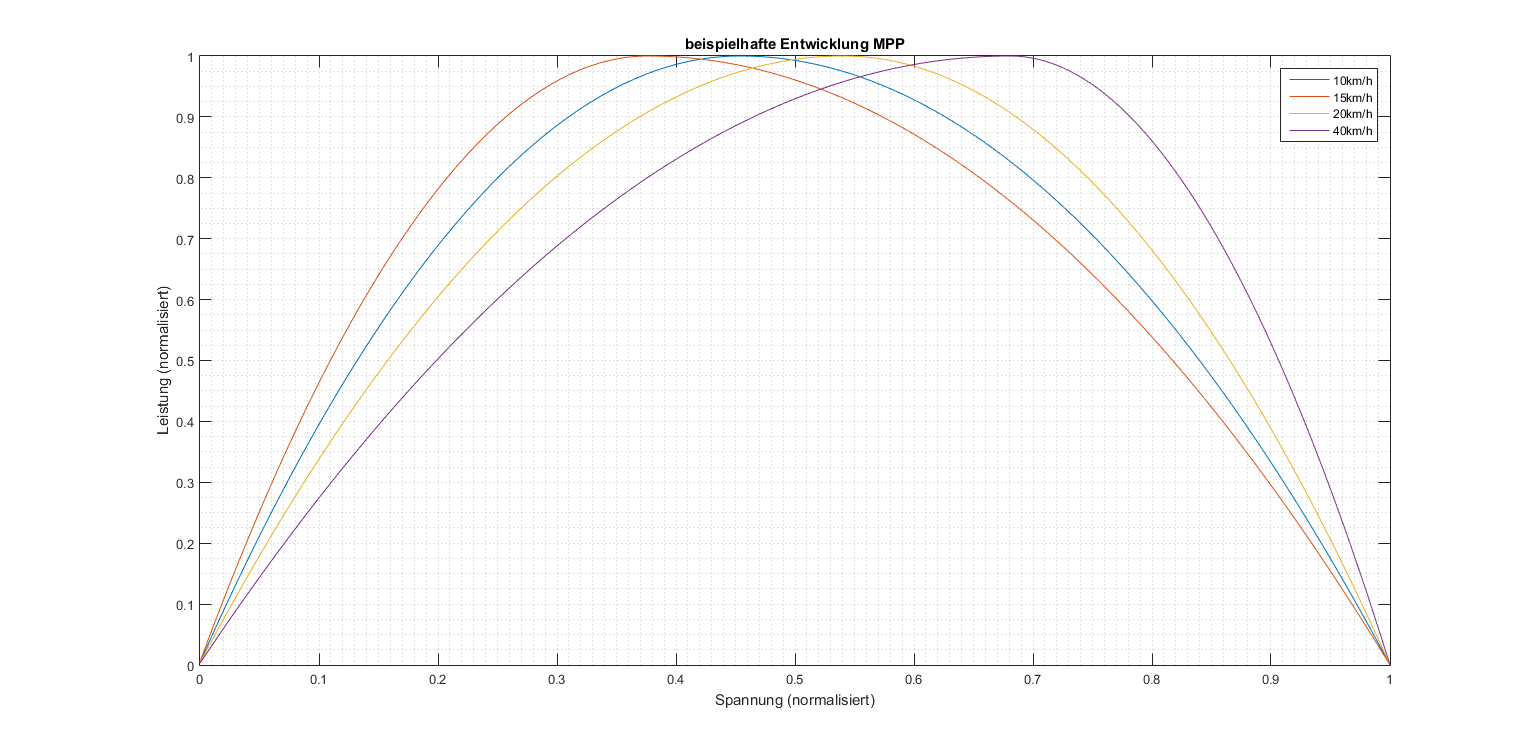
\includegraphics[width=0.5\textwidth]{2TheoretischeGrundlagen/imag/MPPharvesterTheorie.png}
   \caption{MPP Harvester (\cite{MPP_Harv})}
   \label{bild_harvester} 
\end{figure}


% 2.2-------------------------------------------------------------------
\section{Energy Management}\label{t_energy_management} 

Der Harvester des Bicycle Computer erntet eine gepulste Energie im $\mu$W-Bereich. Um diese für eine Applikation zu verwenden, müssen die geringen Energieportionen summiert werden. Sind Energiemengen im mW-Bereich verfügbar, kann die Energie kontrolliert freigegeben werden.

Energy Management bezeichnet das der Energie in Speichern, das Regeln des Inputs, damit die maximale Leistung aus der Quelle bezogen werden kann, das Aufwärtswandeln von Spannung oder Strom auf den geforderten Wert und die kontrollierte Freigabe.

In der Bachelorarbeit ist das Verwenden des Chip EM8500 vorgegeben. Als erstes wird das kontrollierte Energiespeichern anhand dieses Chips erklärt. Danach folgt die Umsetzung des Maximum Power Point Trackings (MPPT) und eine kurze Erklärung der Wirkung des Boosters auf das Energy Managments. Zuletzt wird auf das freischalten von Ausgängen eingegangen, da dies für das Verwenden der Energie die wesentliche Schnittstelle ist. Das Datenblatt des EM8500 ist der CD beigelegt. Der EM8500 ist für Low Power Applikationen entwickelt.

\subsection{Kontrollierte Energiespeicherung}

Bei einer Low Power Harvesting Applikation ist wesentlich, dass vor der Verwendung der Energie, genug Energie gesammelt wurde. Umgesetzt wird dies, in dem die Freigabe der Energie an eine Applikation, VSUP, erst nach dem Erreichen eines gewissen Ladezustands erfolgt. Der Ladezustand des Primärspeichers ist mit VSTS in der Abbildung \ref{em_grundprinzip}.

\begin{figure}[ht]
   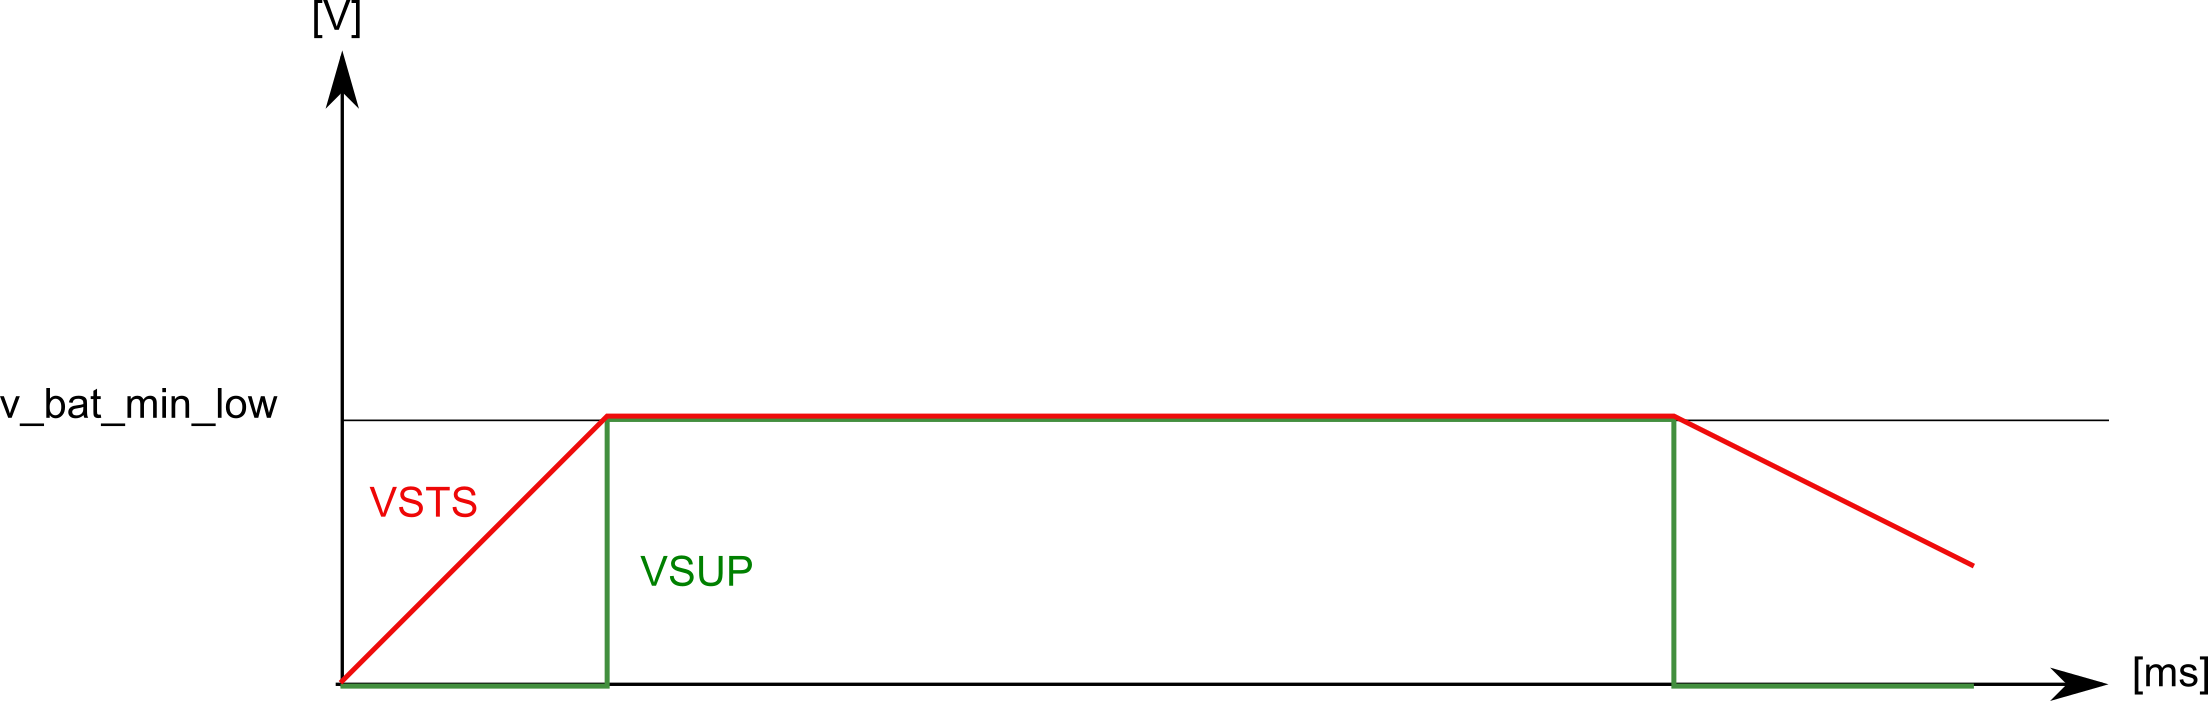
\includegraphics[width=0.5\textwidth]{2TheoretischeGrundlagen/imag/levelMitSTsTheoriel.png}
   \caption{Grundprinzip Applikationsspeisung }
   \label{em_grundprinzip} 
\end{figure}

Im EM8500 wird dies folgendermassen umgesetzt (Abbildung \ref{em_grundprinzip_em8500}): Erreicht der Primärspeichers STS den Schwellwert v\_bat\_min\_low, wird VSUP mit der eingestellten Spannung gespiesen. Die Applikation sollte nicht alle Energie verbrauchen, sodass sich der Speicher weiter lädt. VSUP folgt der Speicherspannung. Verbraucht die Applikation viel Energie, fallen VSUP und VSTS parallel. Speiste der Harvester viel Energie, steigt bei beiden die Spannung an. Unterschreitet VSTS/VSUP den Schwellwert von v\_bat\_min\_low, so wird die Speisung der Applikation gestoppt.


\begin{figure}[ht]
   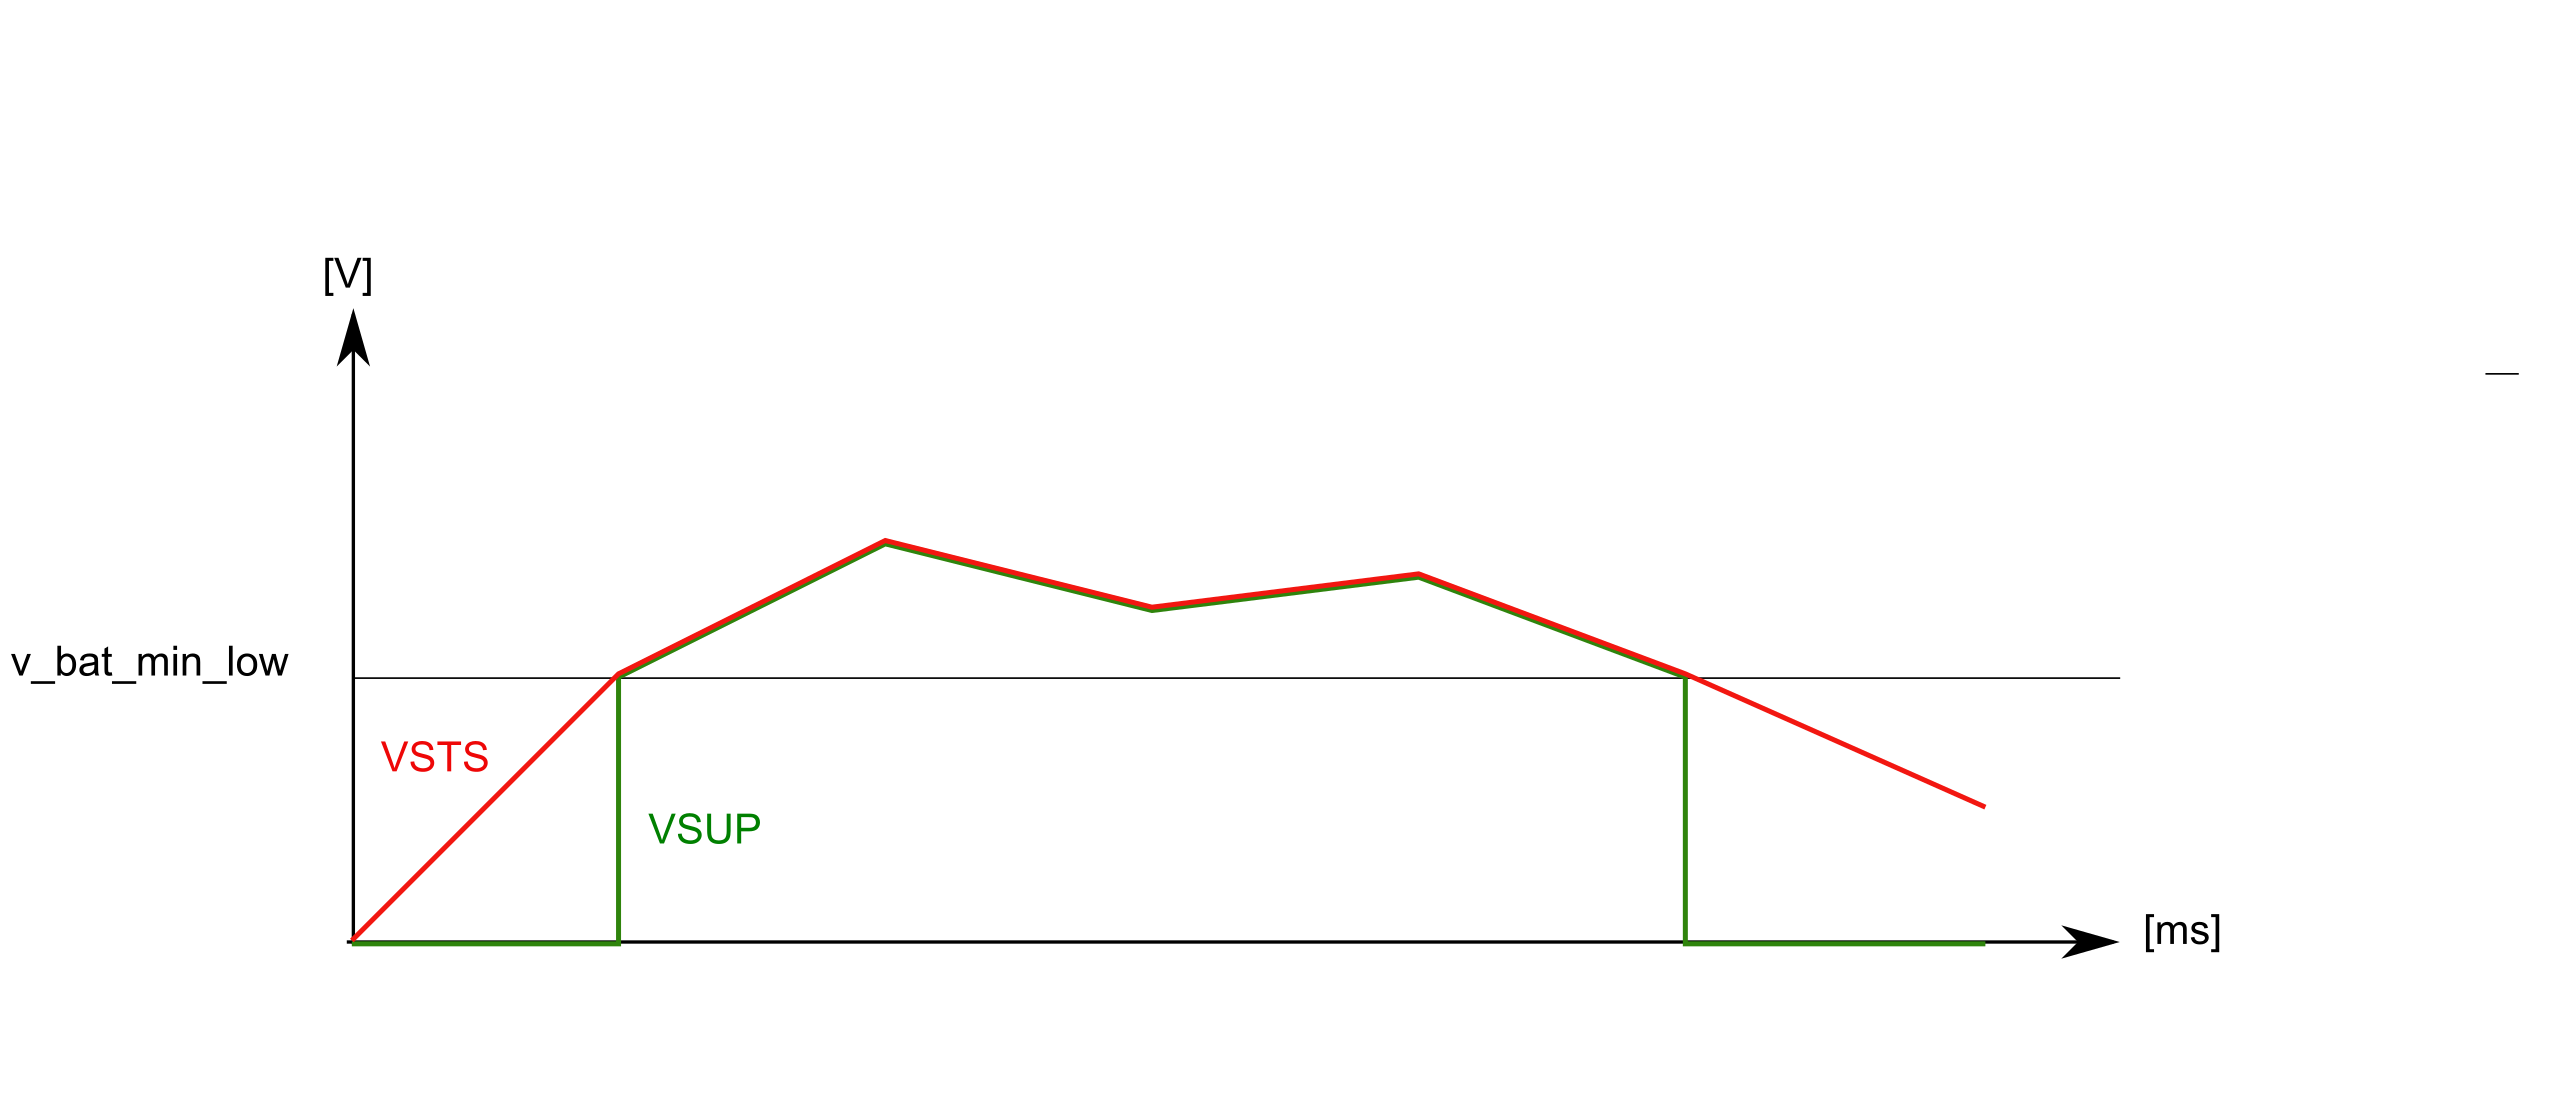
\includegraphics[width=0.5\textwidth]{2TheoretischeGrundlagen/imag/levelSTSReal.png}
   \caption{Applikationsspeisung EM8500}
   \label{em_grundprinzip_em8500} 
\end{figure}

Der Primärspeicher STS ist für die kurzfristige Speisung der Applikation verantwortlich. So bedeutet STS Short Time Storage. Für das lanfristige, sichere Ausführen braucht das System ein Long Term Storage (LTS). Seine Aufgabe ist, Reserveenergie aufzubauen. Diese überbrückt die Energieengpässe, wenn der Harvester zu wenig Energie liefert.
VLTS wird geladen, wenn der Schwellwert bei v\_appl\_max\_los ist (siehe Abbildung \ref{energiespeisung_lts}).

\begin{figure}[ht]
   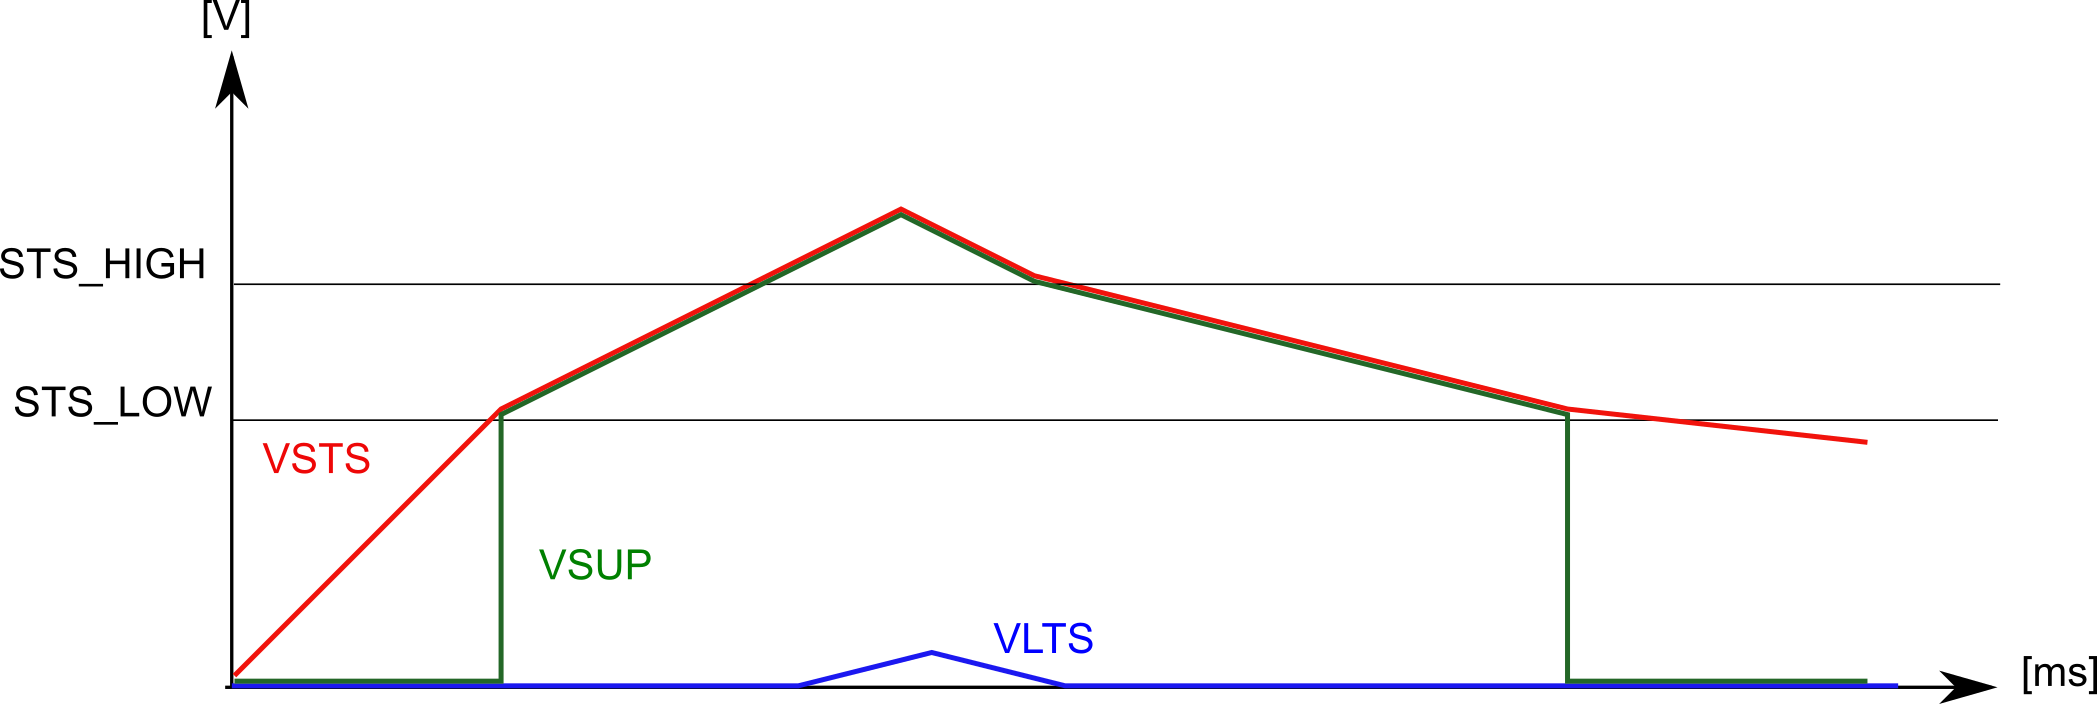
\includegraphics[width=0.5\textwidth]{2TheoretischeGrundlagen/imag/levelMitLTS.png}
   \caption{Sicheres Betreiben durch Long Term Storage}
   \label{energiespeisung_lts} 
\end{figure}

Im Datenblatt des EM8500 \cite{datasheet_EM85} sind weitere Feineinstellungen beschrieben und drei Application Notes helfen bei der Berechnung der Schwellwerte für ein sicheres betreiben. Die Dateien sind auf der CD abgelegt.

Grundsätzlich ist zur Berechnung der Speicher und den Schwellwerten zu sagen, dass der erste Schwellwert (v\_bat\_min\_lo), bei dem die Speisung der Applikation beginnt, genug Energie für die Initialisierung der Applikation gesammelt haben muss. Zudem muss das Abschalten von VSUP vermieden werden. Denn ein Neustart braucht aufgrund der Initialisierung viel Energie und ist ein unnötiger Kraftakt in einem Low Power System. In den Beispielkonfigurationen des Herstellers (\cite{datasheet_EM85} S. 5 - 8 ) sieht man, dass in deren Überlegungen VSUP nicht abgeschaltet wird. Der Hersteller geht davon aus, dass sogar bei dem Freischalten von VSUP die Spannung am STS nicht aufgrund der Last der Applikation fällt, sondern sich weiterhin auflädt.

\begin{figure}[ht]
   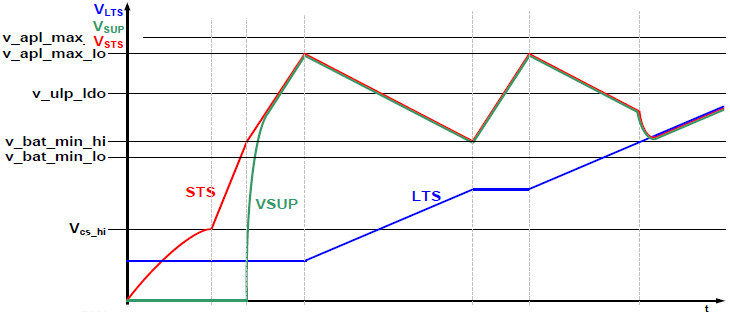
\includegraphics[width=0.5\textwidth]{2TheoretischeGrundlagen/imag/KonzeptFirma.png}
   \caption{Konzept Hersteller (\cite{datasheet_EM85})}
   \label{energiespeisung_lts} 
\end{figure}


\subsection{Regelung des optimalen Leistungsbezugs}
\label{optimaleLeistung}

Wichtigster Punkt in der Energieoptimierung ist, das Maximum aus der produzierten Energie weiterzuverwenden. Aus diesem Grund wird vor Inbetriebnahme eine Leistungskurve des Harvesters erstellt. Wie in Unterkapitel \ref{harv_diff} beschrieben, unterscheidet sich der Maximum Power Point (MPP) unter den Harvestern stark.

EM8500 versucht die Quelle stets in der Nähe dieses Optimums zu betreiben. Dies geschieht über eine Innenwiderstand-Regelung, sodass die Eingangsleistung möglichst dem MPP entspricht. Wie schnell die aktuelle Leistung überprüft wird, ist einstellbar. Der EM8500 besitzt eine Auflösung von 37 mV. Die Abbildung \ref{RegelungSpannung} zeigt das periodische Messen des (unregulierten) Spannungswert des Harvesters. Da die Kurzschlussmessung für das Messen des Stromwerts eine Spannungsspitzen verursacht, sollte die Leistungsüberprüfung nicht zu oft geschehen. In der Abbildung \ref{RegelungSpannung} beträgt die Periode 8 s.

\begin{figure}[ht]
    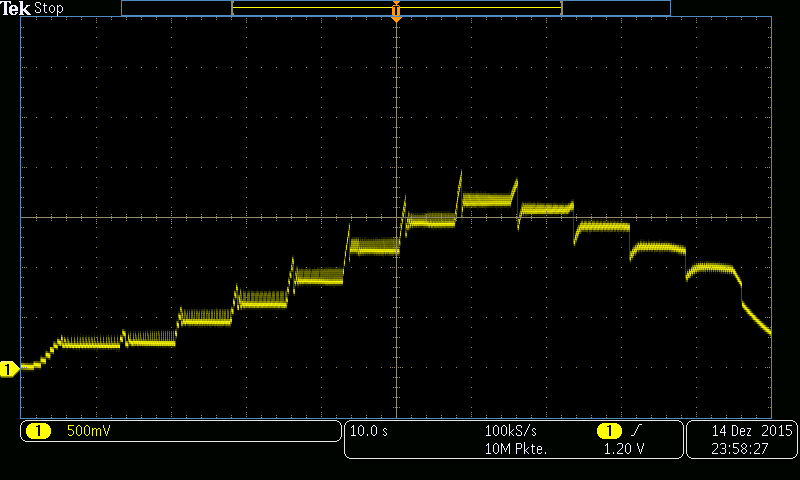
\includegraphics[width=0.5\textwidth]{2TheoretischeGrundlagen/imag/RegelungVHRV.png}
    \caption{Leistungsmessung des Harvesters}
    \label{RegelungSpannung} 
\end{figure}


\subsection{Booster definiert Spannung}

Direkt mit dem MPP-Kontroller ist der Booster (siehe Blockdiagramm im Anhang \ref{anhang_em8500}). Die Aufgabe des Boosters ist es, das interne Spannungsniveau (VREG) zu heben. Der Booster arbeitet ab einer Eingangsspannungen von 0.3 V. Danach regelt er in Schritten von 0.3 V. 

\subsection{Energiezustand kennen und In- und Ausgänge schalten}

Da der Primätspeicher STS vom Boosterausgang gespiesen wird, entspricht dessen Spannung dem des geregelten Boosterausgangs. Für die Berechnung der Speicher muss der Energieverbrauch der Applikation und die Ausgangsspannung des Boosters bekannt sein:

\begin{equation}
  E_{Applikation}= C_{STS} \times \frac{1}{2}\, V_{Booster}
\end{equation}
 
( $E_{Applikation}$ bezeichnet die  minimale Energie, die die Applikation braucht, also mindestens die Initialisierung der Applikation.) Da aus dem Speicherwert in Farad und desssen Spannung der aktuell gespeicherte Energiezustand berechnet werden kann, lässt sich der Schwellwert für das Freischalten der Ausgangs VSUP zur Speisung der Applikation berechnen:

\begin{equation}
v\_bat\_min\_low - V_{SUP} = \sqrt{\frac{2\, \times \, E_{Applikation}}{C_{STS}}}
\end{equation}

Der Grundpegel von $V_{SUP}$ muss abgezogen werden, da sich der Speicher nicht auf 0 entlädt.

Neben VSUP kann der EM8500 drei weitere Ausgänge freischalten: VAUX[0] bis VAUX[2] (siehe Abbildung  \ref{IOEM8500}). Vor allem aber kann per I2C oder SPI der aktuelle Spannungspegel der Regelung (VREG), die Speicher (VDD\_STS und VDD\_LTS)und des Harvestereingangs (VDD\_HRV) abgefragt werden. So kennt die Applikation jederzeit den aktuellen Energiezustand der gesammelten Energie.

EM8500 stellt zwei digitale Überwachungssignale zur Verfügung:\\ 
Der Ausgang HRV\_LOW ist auf logisch '0', wenn die Eingangsspannung vom Harvester grösser als 0.3 V ist. Fällt diese darunter, geht HRV\_LOW auf logisch '1'.
Der Ausgang BAT\_LOW zeigt die Zeitdauer an, in der nur STS die Applikation speist:

\begin{itemize}
     \item BAT\_LOW = '0'\\
           Nicht genügend Energie zur Speisung der Applikation.
           VSUP ist ausgeschalten.
     \item BAT\_LOW = '1'\\
           Genügend Energie zur Speisung der Applikation.\\
           VSUP ist eingeschalten.
      \item BAT\_LOW = '0'\\
           Genügend Energie zur Speisung von LTS.\\
           VSUP ist eingeschalten.\\
           Der Zustand entspricht nicht mehr BAT\_LOW.   
\end{itemize} 

Mit den zwei digitalen Signalen kann der Energiezustand grob abgebildet werden.

\begin{figure}[ht]
    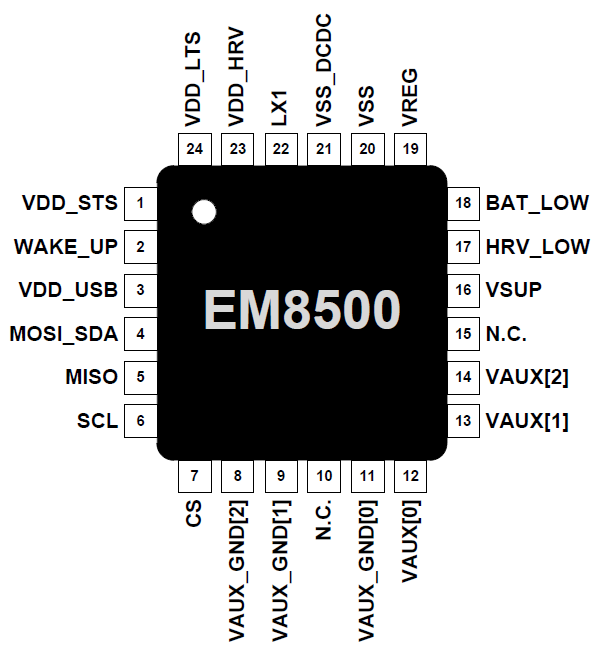
\includegraphics[width=0.5\textwidth]{2TheoretischeGrundlagen/imag/EM8500IO.png}
    \caption{In- und Outputs EM8500  (\cite{datasheet_EM85}, p.11)}
    \label{IOEM8500} 
\end{figure}



% 2.3-------------------------------------------------------

\section{Power Management}\label{t_power_management} 

Die Aufgabe des EM8500-Chip ist es, Energie zu sammeln und kontrolliert frei zu geben. Die Aufgabe das nachfolgenden Microkontrollers ist es, die freigegebenen Energieportionen optimal zu verwenden. Das bedeutet, möglichst wenig Energie bei der Datenverarbeitung zu benötigen. Dies wird durch Abstellen aller unnötigen Microkontroller-Bereiche erreicht und einem zusätzlichen Schlafen während allen Warteprozessen.

In diesem Kapitel werden drei Konzepte zum Umsetzen eines Low Power Systems vorgestellt. Das Hautpthema ist das Schlafen zwischen allen Prozessen. Dies wird im ersten Unterkapitel beschrieben. Das Schlafen bedingt ein Aufwecken aufgrund von Ereignissen. Dadurch ergibt sich eine Interrupt Driven Applikation. Diese wird im zweiten Unterkapitel erklärt. Als letztes dient ein Design Aspekt: Durch das Einbauen einer State Machine über alle laufenden Interrupts, ist es nachfolgenden Entwicklerinnen und Entwicklern einfacher, den Code und die gegenseitigen Beeinflussungen zu verstehen. Dies wird im Unterkapitel beschrieben.

Vor der technischen Beschreibung der Konzepte in den drei Unterkapiteln wird kurz auf die verwendete Hardware eingegangen. In der Bachelorarbeit war als Microkontroller das Simple Link Sensortag von Texas Instrument vorgegeben. Der Grund für dieses Board ist, dass das Sensortag drei Anforderungen auf einem Borad vereint:

\begin{itemize}
    \item Ein Cortex M3 dient als Haupt-Microkontroller und ist aufgrund seiner hohen, und somit schnellen, Rechenleistung und seiner Low Power-Fähigkeiten für eine Harvester-Anwendung wie der Bicycle Computer geeignet.
    \item Auf dem Board ist ein zweiter Cortex M0 für die Wireless-Anbindung angeschlossen. Die Schnittstelle zum Low Power Datensenden ist bereits aufgesetzt. Neben Bluetooth Low Energy kann auch Zigbee verwendet werden.
    \item Auf dem Board sind 10 Sensoren angebunden.
\end{itemize}

Die Funktionsblöcke des Sensortags befinden sich im Anhang \ref{anhang_sensortag}.

\subsection{Einbauen von Schlaufmodi}\label{pm_sleep} 

(Low Power Microcontroller können Gebiete des Prozessors oder von Periopherieelementen temporär ausschalten. Das System befindet sich im Standby Modus. Nur die für die Applikation unabdingbaren Aktivitäten laufen mit niederstem Takt weiter. Über Interrupts können einzelne Bereich aufgeweckt werden, die ihre Aktionen ausführen und danach geht das System wieder in den Standby Modus.)


Dass Prozessoren nach längerer Zeit ohne externen Input in den Schlafmodus gehen, ist Usus (Allgemeingut, bekannt). Bei einer Low Power Applikation geht der Prozessor jedoch nach kleinsten Ausführungsblöcken direkt wieder schlafen. So gehört zu jedem Aufwecken einer Peripherie, der Parallele Schlafmodus, bis dass die Peripherie gestartet ist. (Dies gilt auch für die Sensoren.) In diesem Unterkapitel werden zwei Umsetzungen des Sleep-Moduses konzeptionell erklärt.

\subsubsection{Schlafen zwischen Ausführungen}

Die Abbildung \ref{sleep_Grundprinzip} zeigt das Grunprinzip. Das Programm besteht aus verschiedenen Aktionsblöcken. Diese dauern unterschiedlich lang und verbrauchen unterschiedlich viel Energie. Zwischen den Aktionen ist eine frei wählbare Wartezeit einbaubar ($\Delta$ t0 - t3). Die graue Markierung in jedem Aktionsblock sind die Initialierungen vor jeder Aktion.

Während der Schlafenszeit sind alle Periphierien abgeschalten und im Prozessor (hier als Bsp. Cortex M3) wird nur die Konfigurationen im Flash regelmässig "refreshed". (Zu den unabdingbaren Aktivitäten eines laufenden Microcontrollers gehört das Refreshen (Neuladen) der Register mit den Systemeinstellungen. Diese Refreshing-Peaks sieht man im Standby Modus.)  Dies ist in der Abbildung \ref{sleep_Grundprinzip} an den grünen Spannungsspitzen zu sehen. Ohne "refreshen" des Speichers, gehen die Konfigurationen verloren und vor jeder Aktion muss das System neu komplett initialisert werden.

\begin{figure}[ht]
    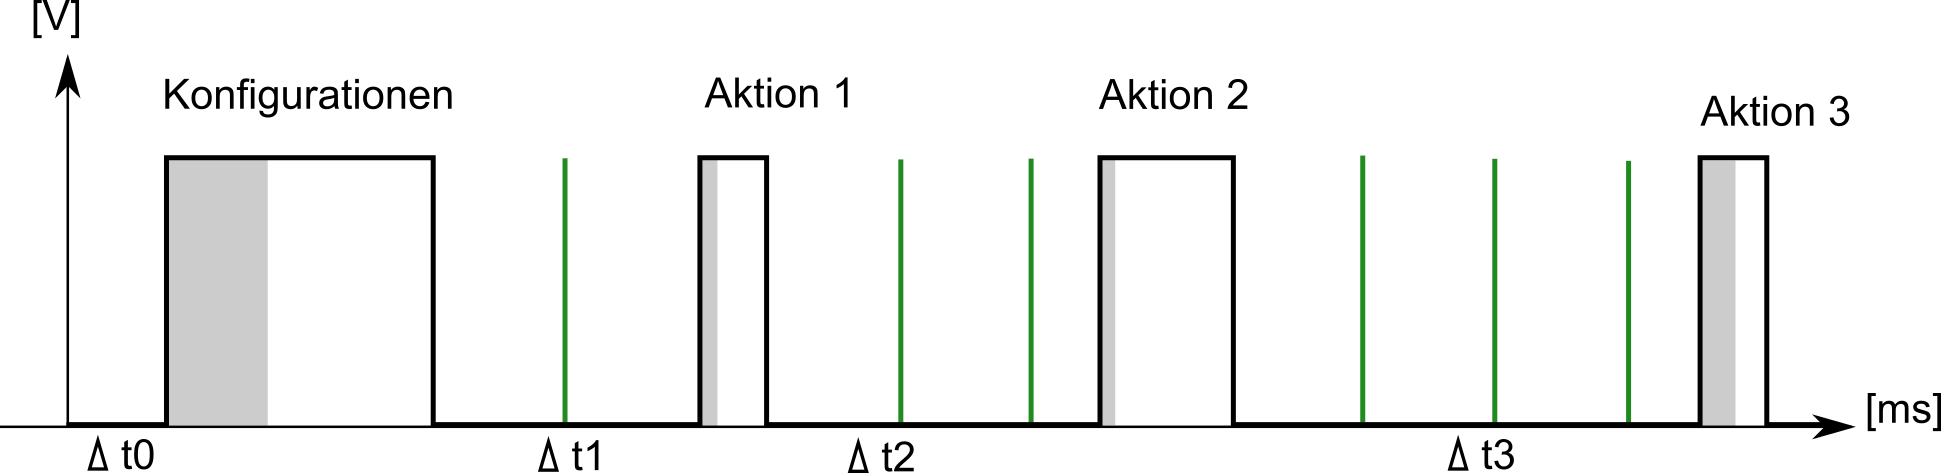
\includegraphics[width=\textwidth]{2TheoretischeGrundlagen/imag/SleepGrundprinzip.png}
    \caption{Schlafen zwischen Ausführungen}
    \label{sleep_Grundprinzip} 
\end{figure}

\subsubsection{Schlafen innerhalb einer Aktion}
Bei einer Applikation im $\mu$ - oder mW-Bereich wird bei jedem Warteprozess, wie z.B. die Zeit, die der Sensor zum Aufwachen braucht, in den Sleep-Mode gegangen. Innerhalb des Codes dominieren die Aufwach- und Abstell-Einstellungen. Für jede Aktion, wird nur die PowerDomain dieser Funktionialität eingeschalten und nach ausführen der Aktion wieder abgeschalten. Die Abbildung \ref{sleep_intern} zeigt dieses Prinzip mit UML dargestellt.

\begin{figure}[ht]
    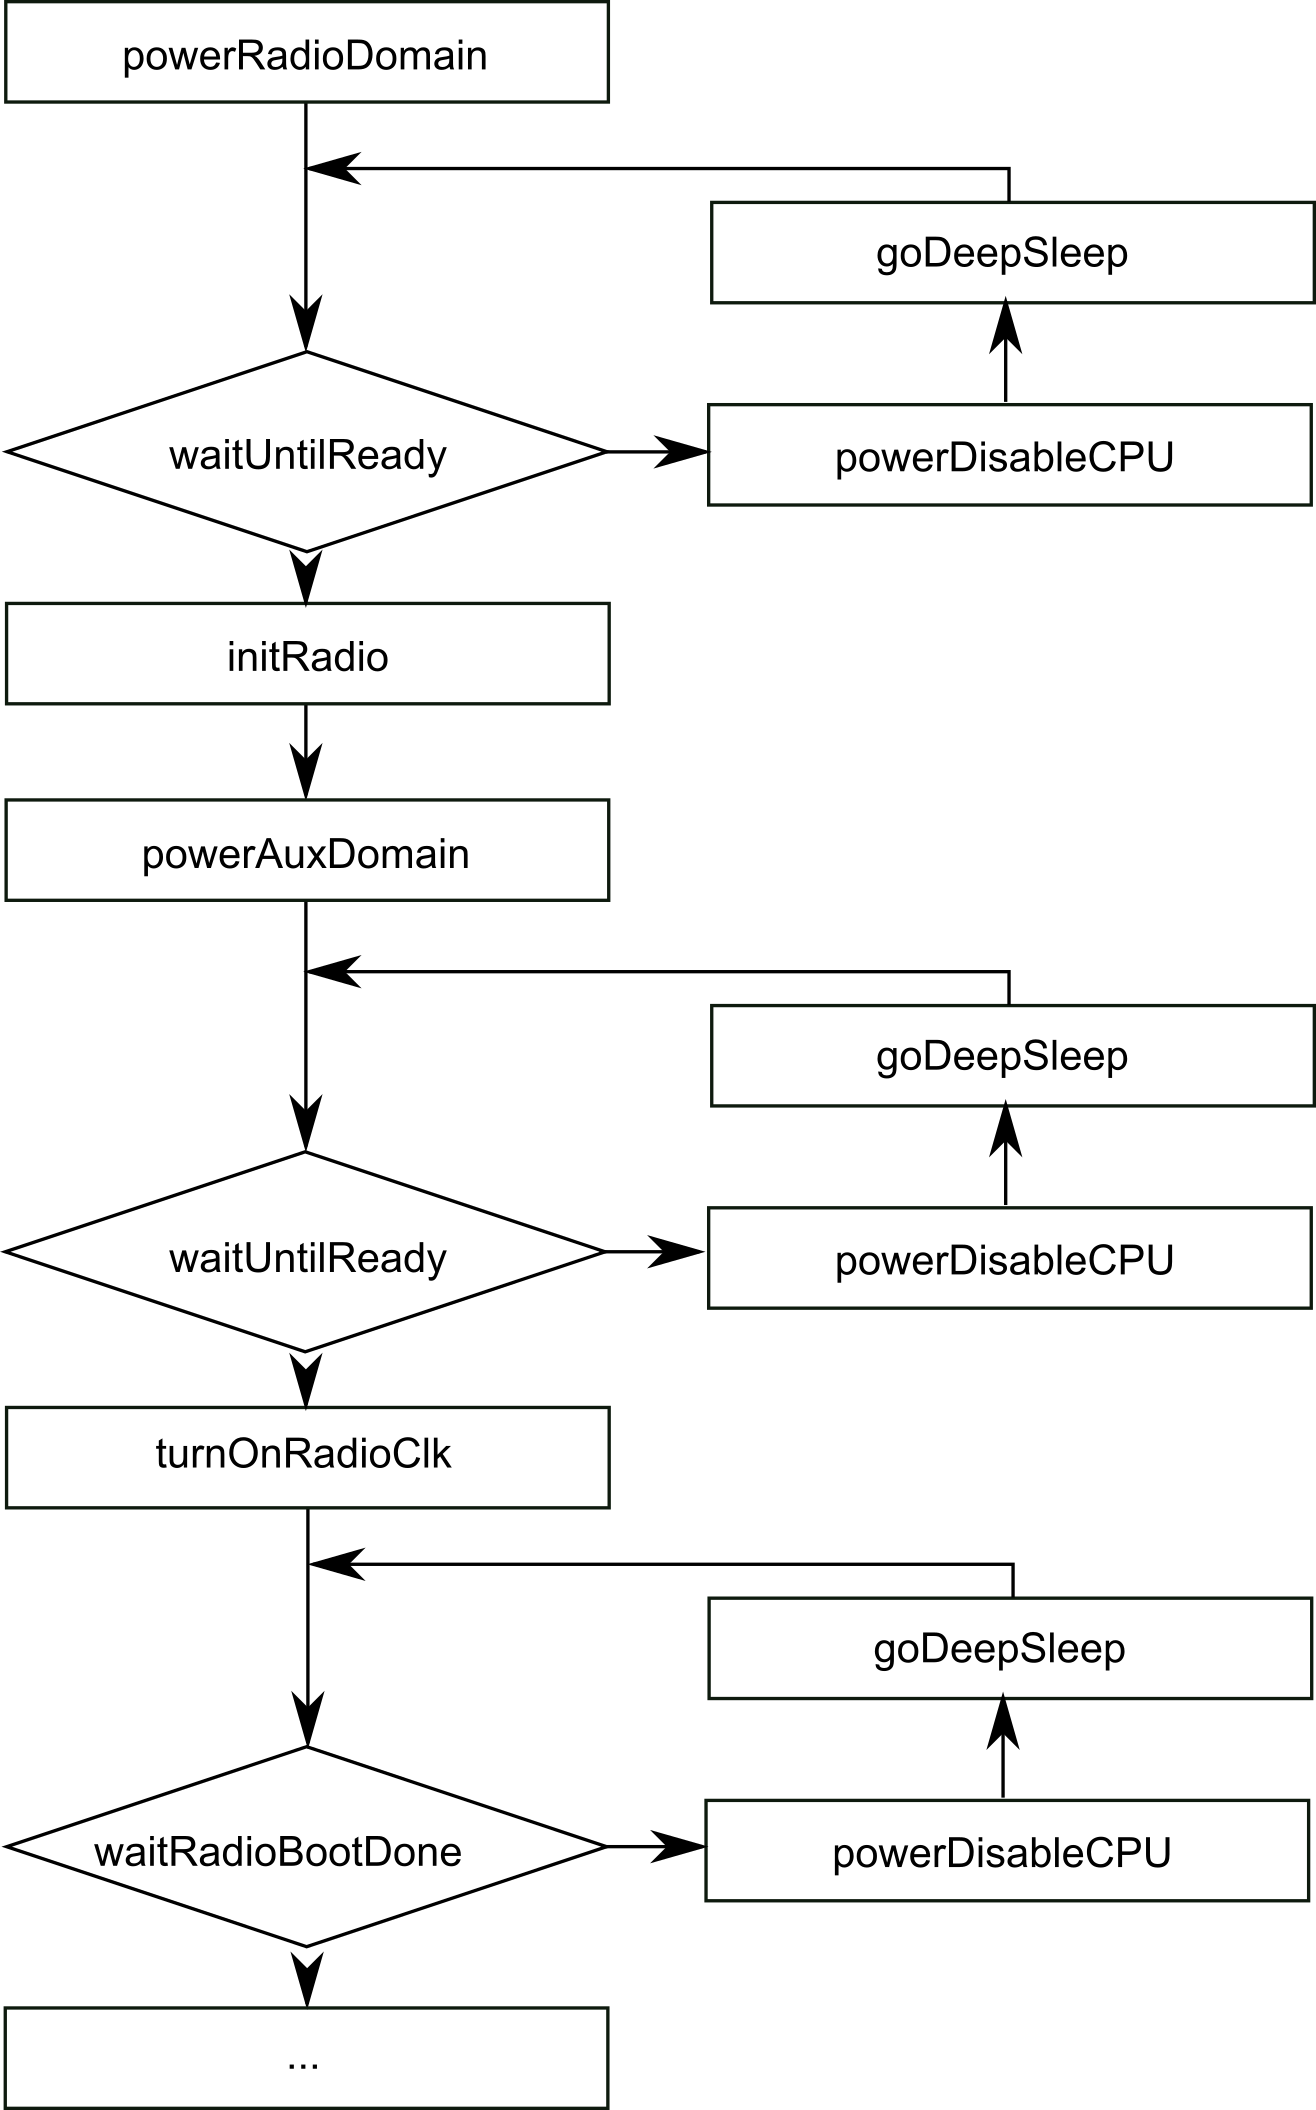
\includegraphics[width=0.5\textwidth]{2TheoretischeGrundlagen/imag/SleepInFunktion.png}
    \caption{Schlafen innerhalb des Codes}
    \label{sleep_intern} 
\end{figure}


\subsection{Interrupt Driven Appliacation}\label{pm_interrupt} 
Zum Schlafen gehört auch ein Aufwachen. Dies ist ein nicht-triviales Problem, lässt sich mit Interrupts lösen. In diesem Unterkapitel werden zwei Konzepte einer Interrupt Driven Applikation erklärt: fixes Aufwachen aufgrund interner Interrupts und asynchrones Aufwachen aufgrund externer Events.

\subsubsection{Aufwachen durch interne Interrupts}
Ein System kann intern seine Signale auswerten und aufgrund kombinatorischen Logik, dem erreichen eines Schwellwerten oder dem Ablaufen eines Timers aufwachen. Solche Wakeups sind fix und unabhängig von äusseren Einflüssen. Ein System mit internen Interrupts ist determinierbar. Das heisst, der Empfang interner Interrupts ist präzis (nur 1 malig und kein Prellen) und kann über Prioritäten gut geregelt werden.

\subsubsection{Aufwachen durch externe Events}
Der Prozessor, oder Teile davon, können auch aufgrund äusserer Impulse aufwachen. Die Verarbeitung des Interrupts ist dieselbe, nur weiss man nicht, wann das Ereignis auftritt. Die Gefahr, dass zwei Interrupts zur selben Zeit eintreffen oder eine Quelle mehrere Interrupts sendet, ist gegeben. Das Löschen der eingegangenen Interrupts und das Prüfen, ob ein Event nicht zu oft verarbeitet wird, muss bewerkstelligt werden. Löst eine Quelle Interrupts über längere Zeit aus, kann dies das System absorbieren und schlimmstenfalls den Systemablauf aus dem Rhythmus bringen.

\subsection{State Machine für definierte Abläufe}\label{pm_state_machine} 
Low Power Applikationen enthalten viele Interrupts. Jede grössere Tätigkeit braucht das Aktivieren mehrerer Schnittstellen, die alle aufgeweckt und aufeinander abgestimmt werden. Da die Codeausführung nicht sequentiell verläuft, sondern Ausführungen in den Interrupt-Handlern stehen, ist ein Überblick der Abhängigkeiten nicht einfach ersichtlich. Um unerwünschte Effekte zu vermeiden, kann eine State Machine implementiert werden. Diese stellt sicher, dass nur aufgrund von gewissen Signalen, ein Aktion ausgeführt wird. Alle anderen Effekte werden ignoriert. Die Abbildung \ref{t_stateMachine} zeigt die definierte Abhängigkeiten durch eine State Machine.

\begin{figure}[ht]
    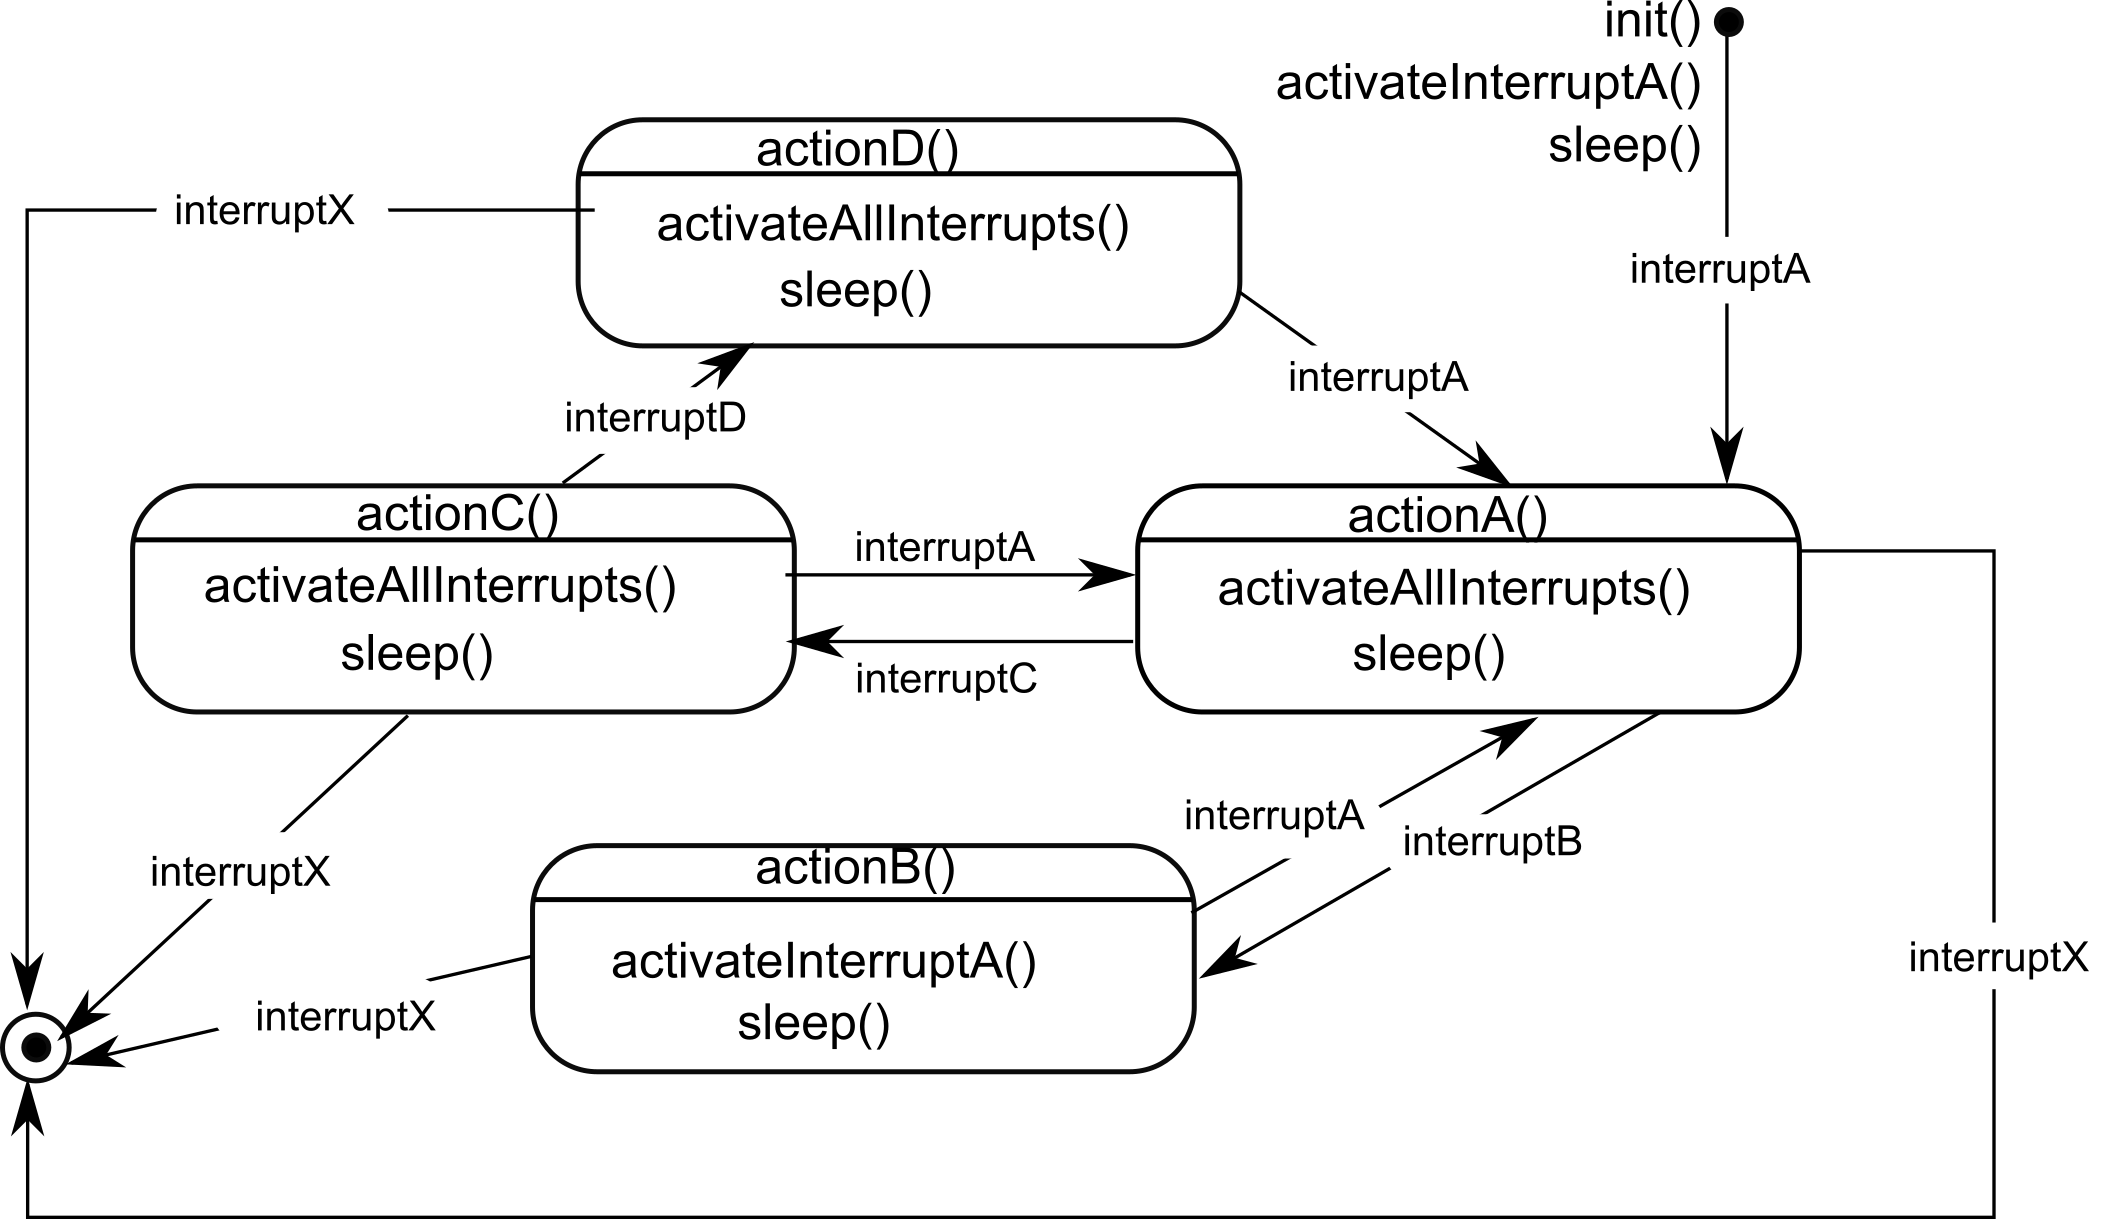
\includegraphics[width=1.0\textwidth]{2TheoretischeGrundlagen/imag/StateMachineGrundlage.png}
    \caption{Struktur durch State Machine}
    \label{t_stateMachine} 
\end{figure}

% 2.4-------------------------------------------------------------------
\section{Bluetooth Low Energy}\label{t_ble} 

Bluetooth Low Energy (BLE) bezeichnet eine Funktechnik, welche es ermöglicht, Daten zwischen Geräten auszutauschen. Der Vorteil von Bluetooth Low Energy ist der niedrigere Energieverbrauch im Gegensatz zum traditionellen Bluetooth. Das Bluetooth Low Energy Protokoll gehört zum Bluetooth Core Specification Version 4.0, wo auch das Classic Bluetooth Protokoll und das Bluetooth High Speed Protokoll enthalten sind. Die Bluetooth Core Specification Version 4.0 ist besser unter dem Namen Bluetooth Smart bekannt und wurde im Juli 2010 veröffentlicht (\cite{youtube_BLE}).

\subsection{BLE im Vergleich zu Bluetooth}
  
Bluetooth Low Energy verwendet das gleiche Frequenzband wie das traditionelle Bluetooth, jedoch sind nur 40 Kanäle à 2 MHz verfügbar, anstatt 79 Kanäle à 1 MHz beim traditionellen Bluetooth. Ausserdem verbraucht BLE, wie der Name bereits indiziert, weniger Energie als andere Übertragungsmedien. So sendet BLE mit maximal 10 mW, was einer Reichweite von ca. 10 Metern entspricht im Gegensatz zu Klasse 1 Bluetooth-Geräten, welche mit 100 mW eine Reichweite von rund 100 Metern erreichen. Ein der BLE-Technik ist, dass die Bauteile für eine BLE-Kommunikation relativ günstig sind und damit die Geräte ebenfalls günstiger hergestellt werden können (\cite{Interent_BLE}, Abschnitt Bluetooth Range).

\subsection{Advertising und Connected Mode}
BLE wird vor allem für batterielose Sensoren verwendet, welche die Energie aus der Umwelt beziehen. Diese Sensoren arbeiten meist als Beacon, was bedeutet, dass sie Daten senden, ohne eine aktive Verbindung mit einem Gerät aufzubauen oder nur eine Verbindung auf Anfrage eingehen, diese jedoch nach kurzer Zeit wieder beenden. Dieser Modus nennt sich Advertising Mode, was vom Englischen advertisement stammt, es soll aussagen, dass der Beacon eine Werbung aussendet und diese nicht auf eine spezielle Person zugeschnitten ist, sondern an die breite Masse gesendet wird.

Eine aktive Verbindung ist bei den meisten Sensoranwendungen auch nicht notwendig, da die Daten einfach gesendet werden können und das empfangende Gerät entscheidet was mit den vorliegenden Daten gemacht wird, wenn das Gerät mehr Informationen benötigt kann eine Verbindung aufgebaut werden. Trotzdem kann mit BLE eine aktive Verbindung eingerichtet werden, jedoch verbraucht eine aktive Verbindung mehr Energie, da Daten gesendet und empfangen werden müssen. Das bedeutet der Sensor kann nicht in einen Standby- Modus gehen, in welchem weniger Energie verbraucht wird, da auf ankommende Daten gewartet wird (\cite{BLE_advertising}).

\subsection{BLE Pakete}

%- Aufbau
%- Maximale Datenlänge  (auf diese verweisen in dem Vorgehen. Alle Daten können problemlos in 1 Pakete versandt werden. Mehrere Sensoren brauchen nicht mehrere Pakete.)
Der Aufbau eines BLE Pakets ist überschaubar. Als erstes wird ein Preamble, bestehend aus abwechselnden 1 und 0, womit der Empfänger sich auf die richtige Frequenz synchronisieren kann. Diese Preamble wird auf dafür verwendet die Verstärkung des Empfängers einzustellen, dies kann sehr wichtig sein bei Signale, welche von einer grösseren Distanz versendet werden, da eine falsche Verstärkung des Signals in Fehlern resultieren kann.

Anschliessend wird die Access Address verschickt, anhand dieser Adresse kann der Empfänger die Nachricht einem ganz bestimmten Sender zuordnen und somit entscheiden, ob die Daten vom richtigen Sender kommen oder ob es eventuell nur Störungen waren, welche zufälligerweise eine Preamble dargestellt haben.

Der Header enthält Informationen zum Aufbau der Daten, welche folgen. Es gibt sieben verschiedene Arten von Aufbauten der Daten.
\begin{itemize}
    \item ADV\_IND – general advertising indication
    \item ADV\_DIRECT\_IND – direct connection indication
    \item ADV\_NONCONN\_INC – nonconnectable indication
    \item ADV\_SCAN\_IND – scannable indication
    \item SCAN\_REQ – active scanning request
    \item SCAN\_RSP – active scanning response
    \item CONNECT\_REQ – connection request
\end{itemize}

Nachfolgen wird die Length eingereiht, welche Informationen über die Anzahl Bytes der Daten enthält. Es wird unterschieden zwischen der Länge eines Advertising Pakets und eines Data Pakets. Die Länge eines Advertising Pakets wird mit sechs Bits dargestellt, welche die Werte von 6 – 37 einnehmen können, wo ein Data Paket nur mit fünf Bits arbeitet, welche die Werte 0 – 31 einnehmen können.

Anschliessend werde die Nutzdaten übertragen, welche je nach gewählter Art, einen anderen Aufbau aufweisen. Es können zwischen 0 bis 296 Bits, also 0 bis 37 Bytes übertragen werden. 

Abgeschlossen wird ein Paket mit dem CRC, welcher die Checksumme der Nachricht enthält. Die Checksumme wird über den Header, Length und die Nutzdaten gebildet (\cite{BLE_Book}, Kapitel 7.2).


\begin{figure}[ht]
    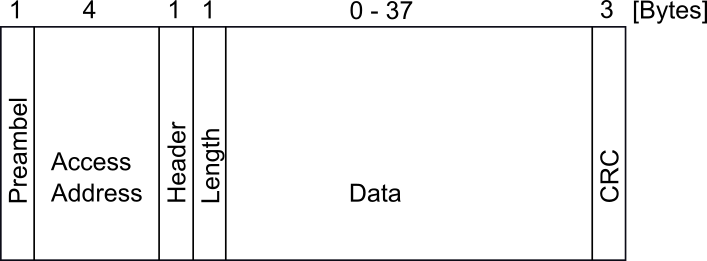
\includegraphics[width=1.0\textwidth]{2TheoretischeGrundlagen/imag/BLEPaketstruktur.png}
    \caption{BLE Paketstruktur}
    \label{ble_paket} 
\end{figure}




\chapter{Vorgehen}
\label{ch_vorgehen} 
Das Ziel ist die Entwicklung eines Prototypen aus dem bestehenden Modell der Projektarbeit von \cite{PA_bicycle}. Die Vorgehensschritte sind in der untenstehenden Auflistung abgebildet. Sie bilden die Struktur dieses Kapitels. Die Definition der konkreten Schritte geschah in Absprache mit Prof. Dr. M. Meli und dem Resarch Assitenten Herr Dario Dünar vom Instiut of Embedded Systems (InES). Auf der CD finden sich die Sitzungsprotokolle über den aktuellen Entwicklungsstand, die offenen Fragen und die Entscheidungen.

\subsubsection*{Liste der Arbeitschritte}
\label{liste} 

\begin{enumerate}
  \item Inbetriebnahme Machbarkeitsstudie  
  \item Hardware entwickeln  
  \item Inbetriebnahme Prototyp      
  \item Energy und Power Management
  \item Entwickeln einer BLE-Applikation       
 \end{enumerate}  

Die sprachliche Unterscheidung von Energy - und Power Management entspricht der Unterscheidung zweier \glqq Management-Teilen\grqq im Prototypen: Das Endprodukt regelt an zwei Stellen auf unterschiedliche Art die zur Verfügung stehende Energie. Der Begriff Energy Management wird in dieser Arbeit für das Sammeln und Weiterleiten von Energie über eine Hardwareimplementation gebraucht. Der Begriff Power Management wird für die Softwareimplementation gebraucht. Diese regelt, dass die zur Verfügung gestellte Energie nicht sofort verbraucht wird. Die sprachliche Trennung ist künstlich, denn in der Umsetzung spielen Hard- und Softwareregelung Hand in Hand. Die sprachliche Unterscheidung dient der Lesbarkeit und bezeichnet keinen physikalischen Unterschied.
 
 
 % 1---------------------------------------------------------------------------
 %------------------------------------------------------------------------------
  
 
\section{Inbetriebnahme Machbarkeitsstudie}\label{v_inbetriebnahme} 

      
Ziel der Inbetriebnahme des Aufbaus der vorangehenden Arbeit \cite{PA_bicycle} ist es, zu definieren, welche Funktionalitäten verbessert werden sollen. Zur Orientierung werden im ersten Unterkapitel \ref{fb} die Funktionsblöcke und deren Aufgaben festgehalten. Danach wird das Verhalten der Vorgängermodells in Unterkapitel \ref{verhalten} ausgemessen. Aus der Analyse entsteht die in Unterkapitel \ref{optimierung} aufgelistete erste Optimierungsliste. Als letztes folgt eine Vertiefung in das auffällige Verhalten des Eingangssignals in Unterkapitel \ref{auffaellig}. Dieser Exkurs hat Ursache in der Begegnung mit  Ives Théoduloz von EM MicroElectronic. Er entwickelte den in dieser Arbeit verwendete EM8500-Chip mit und wies uns auf den auffälligen Signalverlauf des Harvester-Eingangssignals (siehe Abbildung \ref{spannungMachbarkeit}) hin. Dieses Signal wurde deshalb bei der Inbetriebnahme eigens getestet, was im letzten Unterkapitel dokumentiert ist.
      
\subsection{Funktionsblöcke}\label{fb} 

Der Bicycle Computer besteht aus vier Funktionsblöcken, die in der Abbildung \ref{funktionsdiagramm_bild} dargestellt sind. Der erste Funktionsblock ist der Harvester (siehe 1) in der Abbildung \ref{funktionsdiagramm_bild}). Die Aufgaben des Harvesters ist es Energie zu Ernten und dem nächsten Funktionsblock ( Nummer 2) in der Abbildung  \ref{funktionsdiagramm_bild} zur Verfügung zu stellen. Der zweite Funktionsblock wird als Energy Management-Teil in der Arbeit bezeichnet. Die Aufgabe des zweiten Blocks ist es, Energie zu Sammeln und kontrolliert an die Verbrauchsstelle freizuschalten. Detaillierte Informationen finden sich in den Theoretischen Grundlagen im Unterkapitel \ref{t_energy_management}. Der dritte Funktionsblock ist der Ort, an dem die Energie verbraucht wird. In dieser Arbeit dient die Energie dem Betreiben von Sensoren und dem versenden derer Daten. Dies wird auf dem Sensortag (siehe Anhang \ref{anhang_sensortag}) umgesetzt. Der Grund dafür wird in der Einleitung des Kapitels \label{t_power_management} dargelegt. Der letzte Funktionsblock bezeichnet das Ziel, das Erhalten von Sensordaten in einer Applikation.  

\begin{figure}[ht]
   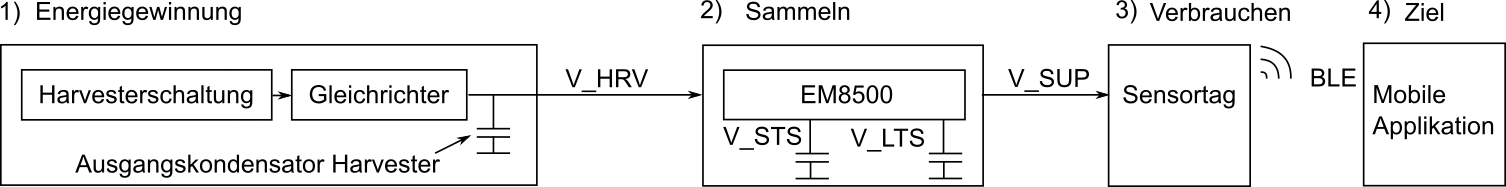
\includegraphics[width=1\textwidth]{3Vorgehen/imag/Blockdiagramm.png}
   \caption{Funktionsblöcke Bicycle Computer}
   \label{funktionsdiagramm_bild} 
\end{figure}

Den Funktionsblöcke sind Spannungsbezeichnungen sowie Kondensatoren beigefügt. Dies, weil bei der Beschreibung des Verhaltens des Vorgängermodells, diese Spannungslevel für die Funktionsbeurteilung wichtig werden. Die nachfolgende Legende beschreibt die Beschriftung näher.

\subsubsection*{Legende Abbildung \ref{funktionsdiagramm_bild} }
\label{legende}
\begin{tabbing}
    Bezeichnung \quad\= Beschreibung\\[0.8ex]
    V\_HRV \> Ausgangspannung Harvesterquelle, Eingangsspannung Energy Management\\
    V\_STS\> Spannung am STS--Kondensator (Primärspeicher)\\
    V\_LTS\> Spannung am LTS--Kondensator (Sekundärspeicher)\\
    V\_SUP\> Ausgangsspannung Energy Managment, Eingangsspannung Sensortag\\
    BLE \> Senden der Daten per Bluetooth Low Energy (siehe \ref{t_ble} \\
\end{tabbing}   
\todo{Header Tabelle (Bezeichnung, Beschreibung) weg } 

\subsection{Verhalten des Vorgängermodells}\label{verhalten} 

Die Inbetriebnahme bestätigte das in der Dokumentation \cite{PA_bicycle} beschriebene Verhalten. Die Abbildung \ref{spannungMachbarkeit} zeigt den zeitlichen Verlauf der Energiestände zwischen den Funktionsblöcken (siehe Abbildung \ref{funktionsdiagramm_bild} und an den Speicherelementen. Die Legende zur Abbildung  \ref{spannungMachbarkeit} erklärt die Signale.

\begin{figure}[ht]
    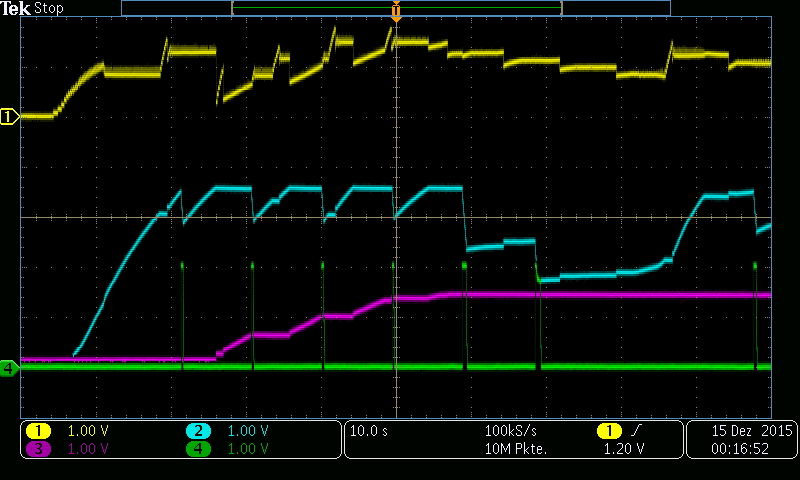
\includegraphics[width=0.5\textwidth]{3Vorgehen/imag/messungPA.png}
    \caption{Spannungswerte Modell der Machbarkeitsstudie}\label{spannungMachbarkeit} 
\end{figure}

\subsubsection*{Legende Abbildung \ref{spannungMachbarkeit} }
\begin{tabbing}
    Channel\quad\= Farbe\quad\= Beschreibung\\[0.8ex]
    CH1\> gelb\> Spannungsverlauf V\_HRV\\
    CH2\> blau\> Spannungsverlauf am STS--Kondensator\\
    CH3\> violet\> Spannungsverlauf am LTS--Kondensator\\
    CH4\> grün\> Ausgangsspannung nach Energy Management\\
     \>  \>      Eingangsspannung Sensorttag
\end{tabbing}    

Im Folgenden werden die einzelnen Spannungsverläufe chronologisch der Kanalnummer nach analysiert. Kanal 1 spiegelt die Spannung am Harvesterausgang wieder (V\_HRV). Gemäss Theorie \ref{eingangsspannung} bzw. gemäss Datenblatt des EM8500 ist der EM8500-Chip für ein DC-Signal ausgelegt. Er geht von einem regelmässigen Eingangssignal aus und regelt die Spannung auf den MPPT. Diese Regelung sollte wie in Abbildung \ref{RegelungSpannung} aussehen. Das reale Signal entspricht nicht diesem Verhalten. Die Regelung ist abrupt und überspringt mehrere Spannungslevel. Der Ursache für die schlechte Regelung soll nachgegangen werden.

Kanal 2, blau, gibt den Spannungsverlauf am Hauptspeicher, dem Primärspeicher, der in der im Datenblatt von EM8500 STS heisst, wieder. Das Energy Management des Vorgängermodells setzt den Schwellwert für den Primärspeicher (STS) mit 3.6 V hoch (Details zu den Schwellwerten im Kapitel Theoretische Grundlagen \ref{t_energy_management}). Der hohe Wert erklärt durch das Ziel, genug Energie für ein konstantes Paketversenden zu haben. Dies gelingt für fünf BLE-Pakete. Danach reicht die Energie nicht mehr aus. V\_SUP, grünes Signal, wird nicht mehr gespiesen. Nach 30 s ohne Pakete senden ist wieder genug Energie gespeichert, für weitere 5 Datenpakete.

In der Auswertung viel uns auf, dass dieser Signalverlauf nur bei einer Geschwindigkeit gegen 70 km/h möglich ist. Die Speicherkapazität von 470 $\mu$F und ein Schwellwert der Spannung von 3.6 V ist mit normaler Geschwindigkeit (15 km/h) auch nach 30 min nicht zu erreichen. Fährt man gegen 70 km/h so erhält man die in der Abbildung gezeigte Ladezeit von rund 25 s. Eine exakte Geschwindigkeitsmessung ist zu Beginn der Arbeit nicht möglich. Das Rad wird von Hand gedreht und mit einem Metronom wird die Umdrehungsgeschwindigkeit vorgegeben. Bei einem Radumfang von 2.04 m und mit drei Umdrehungen pro Sekunde, erreicht man eine Geschwindigkeit von xxx \todo{ausrechnen} km/h. Da diese Messmethode über längere Zeit nicht sehr genau ist, bestand eine der Aufgabe nach der Inbetriebnahme im Organisieren eines Messaufbaus. Dieser professionellere Messaufbau wird im Anhang \ref{messaufbau} beschrieben.


Kanal 3, das pinkige Signal, zeigt die Spannung am Long Time Speicher. Die Inbetriebnahme zeigt, dass sich der LTS lädt. Es erstaunt jedoch, dass seine geerntete Energie nicht verwendet wird. Der Spannungswert von LTS geht nie herunter.
Die Vermutung ist, dass der eingestellte Schwellwert für den Bezug von Energie von LTS \ref{energiespeisung_lts} nicht stimmt.

Kanal 4, das grüne Signal, zeigt, die Speisung des Sensortags. In Modell der Projektarbeit steuert der Microkontroller des Sensortags den Verbraucht. Alle 10 s wacht das System auf, bezieht Energie vom EM8500-Ausgang für das Senden eines Paketes und geht dann wieder schlafen. Das Aufwachintervall ist fix.


\subsection{Optimierungsliste}\label{optimierung} 

\todo{ Ev. Texbausteine von oben hier hin}

Aus den Messungen der Inbetriebnahme konkretisierten sich die generellen Aufgaben, die in der ersten Liste der Arbeitsschritte zu Beginn des Vorgehens  beschrieben wurden. Folgende vier Punkte sollen durch den Prototypen verbessert werden: 

\begin{itemize}
     \item Der Verlauf des Harvester-Eingangs wechselt abrupt. Der Eingang soll besser geregelt werden. 
     \item Das Laden des Primärspeichers von 470 $\mu$F in 25 s benötigt es eine Geschwindigkeit von mehr als 60 km/h.  Die Harvesterschaltung soll so weiterentwickelt werden, dass bei 10 km/h genug Energie zum Senden von BLE-Paketen besteht.    
     \item Das zweite Speicherelement, der LTS, entlädt sich nicht. Dadurch kann seine Energie nicht verwendet werden. Die Schwellwerte am EM8500 und ev. die Kondensatorenwerte sollen so angepasst werden, dass sich der zweite Kondensator entlädt
     \item Die Energie wird statisch nach einem fixen Zeitintervall von 10 s genutzt. Das Zeitintervall soll der Geschwindigkeit angepasst werden. Bei höherer Geschwindigkeit soll das Intervall kürzer werden.
\end{itemize} 


Im Resultatsteil Kapitel \ref{ch_resultat} werden die Fortschritte in diesen vier Punkten ausgewiesen.

\subsection{Vertiefung in auffälliges Verhalten des Harvestereingangs}\label{auffaellig} 


Text aus Einleitung: Für Argumentation. (Als letztes folgt eine Vertiefung in das auffällige Verhalten des Eingangssignals in Unterkapitel \ref{auffaellig}. Dieser Exkurs hat Ursache in der Begegnung mit  Ives Théoduloz von EM MicroElectronic. Er entwickelte den in dieser Arbeit verwendete EM8500-Chip mit und wies uns auf den auffälligen Signalverlauf des Harvester-Eingangssingals (siehe Abbildung \ref{spannungMachbarkeit}) hin. Dieses Signal wurde deshalb bei der Inbetriebnahme eigens getestet, was im 

??????  .... folgte.) Hier ist nun dieser erwähnte Text.

Vorschlag Katrin:
Die auffällige Regelung des Harvesterinputs wurd Ives Théoduloz gezeigt. 

Gemäss Ives Théoduloz sollten Kondensatoren der Harvesterschaltung im Bereich von 4.7 $\mu$F liegen, sodass die Energiemanagementschaltung ordnungsgemäss funktioniert.  


In der Machbarkeitsstudie ist nach dem Gleichrichter ein Kondensator von 470 $\mu$F nachgeschaltet. Dieser glättet die Spannungspulse nach dem Gleichrichter zu einer DC-ähnlichen Spannung mit Rippeln.

Aus diesem Grund wird die Rippelspannung am Ausgangs der Harvesterschaltung mit kleineren Kondensatoren gemessen. Das Messprotokoll befindet sich im Anhang.

\subsubsection{Ausmessen der Auswirkung des Ausgangskondensators}
\todo{auf Messprotokoll verweisen}

Mit einem Kondensator von 470 $\mu$F wird die Ausgangsspannung der Harvesterspannung fast rippelfrei. Die Rippelspannung beträgt 3.2 mV (siehe Abbildung \ref{kond470uF}).

\begin{figure}
    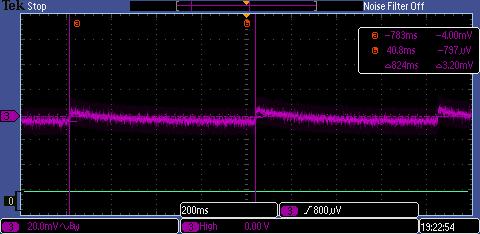
\includegraphics[width=15cm]{3Vorgehen/imag/470uF.PNG}
    \caption{Rippelspannung bei Glättung mit 470 $\mu$F Kondensator}\label{kond470uF} 
\end{figure}

\subsubsection*{Messaufbau}
In der gegebenen Harvesterschaltung wird am Kondensator die Spannung mit einem Kathodenstrahloszilloskop (KO) gemesssen. Ausgehend vom bestehenden Kondensator (470 $ \mu $F), werden danach Elektrolytkondensatoren (Elko) mit den Werten 100 $\mu F $F, 47 $\mu$F und 10 $\mu$F gemessen.

\begin{figure}[h]
    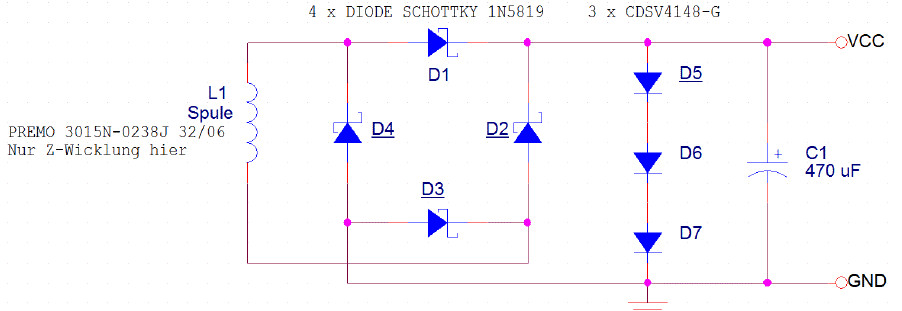
\includegraphics[width=15cm]{3Vorgehen/imag/messschaltungHarvesterschaltung.jpg}
    \caption{Messschaltung}
\end{figure}

\subsubsection*{Resultat}

Die Rippelspannung erhöht sich wie erwartet. Vpp beträgt bei 100 uF \textbf{xx} mV, bei 47 uF 28.8 mV (siehe Abbildung \ref{kond47uF}) und bei 10 uF 320 mV (Abbildung \ref{kond10uF}).
 
\begin{figure}
    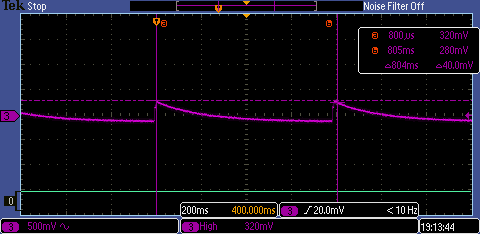
\includegraphics[width=15cm]{3Vorgehen/imag/10uF.PNG}
    \caption{Rippelspannung mit 10 uF Kondensator}\label{kond10uF} 
\end{figure}

\begin{figure}
    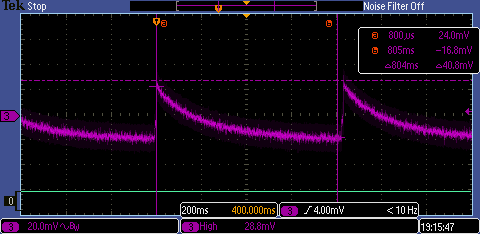
\includegraphics[width=15cm]{3Vorgehen/imag/47uF.PNG}
    \caption{Rippelspannung mit 47 uFKondensator}\label{kond47uF} 
\end{figure}

Nach Rücksprache mit einem Entwickler des EM8500-Chips wird der zu hohe Kondensator vor dem Harvester-Eingang als Ursache vermutet. Laut Datenblatt sollte dieser 4.7 $\mu$F, damit der Booster mit eingebautem MPPT ideal regeln kann.


Aus den Beobachtungen ergaben sich folgende Aufgaben für die Entwicklung des Prototypen:

\begin{enumerate}
    \item Die Harvesterschaltung funktioniert nicht optimal. Die Auswirkung des zu hohen Kondensator vor Harvestereingang soll getestet werden
    \item Die Schaltung soll für eine Geschwindigkeit von 10 km/h ausgelegt werden
    \item Die Konfigurationen beim EM8500 sollen überarbeitet werden, sodass LTS genutzt wird
    \item Das Senden der Pakte soll der Geschwindigkeit angepasst werden
\end{enumerate}

Punkte 1 und 2 haben Auswirkung auf das Layout, Punkte 3 und 4 auf die 





%------------------------------------------------------------------------------
% 2---------------------------------------------------------------------------
%------------------------------------------------------------------------------



\section{Hardware entwickeln}

Notiz: Ziel dieses Artikels gemäss Inbetriebnahme:
- Genug Energie für BLE bei 10 km/h
\subsection{Schema}
\subsection{Bauteildefinition und Optimierung}
\subsection{Layout}

\todo{ Namensklärung: V HRV = VCC}
\todo{Messprotokolle umbenennen}


---- alter Text-----                             
Ein wichtiger Punkt der Arbeit ist die Miniaturisierung der bestehenden Hardware, das heisst der Aufbau aus der Machbarkeitsstudie soll auf eine Leiterplatte gebracht werden. Die Leiterplatte hat einige Vorgaben, welche im besten Fall alle eingehalten werden sollen.

\begin{enumerate}
    \item Die Leiterplatte soll nicht oder nur geringfügig grösser sein als das TI-SensorTag.
    
    \item Alle Netze sollen mit Testpunkten ausgestattet werden.
    
    \item Alle Anschlüsse vom TI-SensorTag sollen auf der Leiterplatte mit Testpunkten ausgestattet werden.
    
    \item Alle Testpunkte vom TI-SensorTag sollen in einem Raster von 2.54 mm angeordnet werden, damit ein Stecker kontaktiert werden kann.
    
\end{enumerate}
	


\subsection{Das Schema (oder der Stromlaufplan)}
Als erstes musste ein Schema, auch Stromlaufplan genannt, gezeichnet werden. Das Schema wurde Blockweise erfasst, als erstes wurde die Harvesterschaltung erfasst. Das Schema wurde aus der Machbarkeitsstudie entnommen. Die Funktionsweise der Harvesterschaltung kann wieder in mehrere Teile unterteilt werden.

\begin{enumerate}
    \item Die Spule: Gewinnt Energie aus dem vorbei schnellenden Magneten.
    
    \item Der Gleichrichter: Erzeugt positive Pulse aus der induzierten Spannung.
    
    \item Der Limiter: Limitiert die Spannung auf eine fixe Spannung.
    
    \item Der Ausgangskondensator: Glättet die positiven Pulse aus dem Gleichrichter.
    
\end{enumerate}

Der nächste Block ist der EM8500-Chip mit seinen Stützkondensatoren. Das Schema wurde aus dem Datenblatt entnommen. 
Die Energiespeicher, welche in dieser Arbeit mittels Elektrolytkondensatoren dargestellt werden, sind einige der wichtigsten Elemente. Die Speicherelemente werden nicht auf der Leiterplatte Platz finden, da die meisten Elektrolytkondensatoren zu hoch sind und der Platz zwischen den Leiterplatten sehr gering ist. 
Die Umlauferfassung wird mit einem Reed-Switch ermöglicht. Der Reedswitch ist einer der kleinsten Blöcke im Schema.
Der Block Interface enthält die Verbindung zum TI-SensorTag, ein Stecker realisiert dieses Interface. Der Stecker ist bereits vom TI-SensorTag vorgegeben, es handelt sich um einen Stecker, welcher sein eigenes Gegenstück darstellt. 

\subsection{Optimierung der Harvesterschaltung}

Nach dem Erfassen des Schemas wurde die Optimierung der Hardware angegangen. Die beste Optimierungsmöglichkeit und auch der kritischste Block ist die Harvesterschaltung, hier wird die Energie für die restliche Schaltung gewonnen. In mehreren Schritten wurden die einzelnen Teile der Schaltung analysiert und versucht zu optimieren.

\subsubsection{Optimierung der Spule}

Die Spule gewinnt die Energie aus dem vorbei schnellenden Magneten, hier kann die gewonnene Energie beeinflusst werden. Eine gute Spule kann mehr Energie aus dem bewegten Magneten gewinnen, wichtig ist die Induktivität L und die Fläche A, welche die Spule hat. Eine Vorgabe war dass die Spule von der Grösse nicht merklich verändert wird, ausser man würde eine kleinere Spule finden, welche mehr Energie gewinnt. Eine Spule mit ähnlicher Fläche bzw. Grösse wurde gefunden, welche eine höhere Induktivität besitzt. Die Spule von Würth Elektronik ist sehr vielversprechend, denn die gleiche Fläche mit höherer Induktivität bedeutet mehr Energiegewinn aus dem Magneten.
\todo{Hier Schlusswort von Messprotokoll einfügen}.

\subsubsection{Optimierung des Gleichrichters}

Der Gleichrichter aus dem Aufbau der Machbarkeitsstudie besteht aus vier Dioden vom Typ 1N5819, diese Dioden sind nicht für eine LowPower-Anwendung ausgelegt. Ausserdem könnte ein Gleichrichter gefunden werden, welcher in einem Gehäuse ausgeliefert wird. Wichtig ist dass der Leckstrom so gering wie möglich ist und die Schwellenspannung ebenfalls möglichst klein bleibt. 
\todo{Hier Schlusswort von Messprotokoll einfügen}.

\subsubsection{Optimierung des Limiter}

Der Limiter ist eine Spannungbegrenzung, da die nachfolgende Schaltung nicht mit einer zu hohen Spannung betrieben werden darf. Dieser Schaltungsteil ist sehr kritisch, denn er darf nicht zu viel Energie verlieren, muss aber trotzdem die Spannung immer begrenzen. Die Spannung darf einen Pegel von 2 V nicht überschreiten, da ansonsten der EM-8500-Chip droht zerstört zu werden. 
\todo{Hier Schlusswort von Messprotokoll einfügen}.

\subsubsection{Optimierung des Ausgangskondensators}

Der Ausgangskondensator muss möglichst niedrig gehalten werden, gemäss Aussage von Yves, da ansonsten der EM8500-Chip Mühe hat den Eingang zu regeln. Trotzdem darf der Ausgangskondensator nicht zu klein dimensioniert werden, da ansonsten die Rippelspannung am Ausgang der Harvestersschaltung zu hoch ist und der EM8500-Chip ebenfalls nicht mehr richtig regeln kann.
\todo{Hier Schlusswort von Messprotokoll einfügen}.


\subsection{Bauteildefinition}

Nachdem das Schema gezeichnet wurde und die Schaltung opimiert wurde, mussten die Bauteile noch definiert werden. Es mussten die Footprints, sowie die Hersteller, Herstellerbezeichnungen, Lieferant und Lieferantenartikelnummer hinterlegt werden. Einige Footprints waren bereits in den Bibliotheken vorhanden, welche wir von Lukas erhalten haben. Fehlende Footprints wurden ergänzt, wie zum Beispiel der Footprint der Spule.


\subsection{Das Layout}

\subsubsection{Positionierung}
Die Positionierung der Bauteile auf der Leiterplatte ist sehr wichtig, da hier schon unnötige Leiterbahnen gespart werden können bzw. die Länge von gewissen Leiterbahnen können extrem verkürzt werden.
Wichtig ist, dass die Stüztkondensatoren bei dem EM8500-Chip so nah wie möglich am Chip platziert werden, damit die Spannungen am Chip so konstant gehalten werden können, wie nur möglich.
Weiter sollte die Harvesterschaltung ebenfalls sehr eng beieinander platziert werden, um zu verhindern, dass durch lange Stromlaufwege bereits Leistung verloren geht. Problematisch ist, dass die Spule auf der unteren Seite der Leiterplatte platziert werden muss, somit wird die Schaltung ein auf zwei Layer aufgeteilt.
Eine grosse Herausforderung ist die Positionierung der Testpunkte, um das Interface zum TI-SensorTag zu realisieren. Dadurch wird ein grosser Platz für die korrekte Positionierung der Testpunkte eingenommen.

\subsubsection{Gestaltung der Leiterbahnen}

Wann immer möglich wurden die Leiterbahnen, welche zu der Harvesterschaltung gehören, mit 20 Mil gezogen, um eine möglichst verlustfreie Leistungsübertragung zu gewährleisten. Alle anderen nicht leistungskritischen Leiterbahnen wurden mit eine Leiterbahnbreite von 10 Mil platziert, um nicht mehr Platz in Anspruch zu nehmen als nötig.

\subsubsection{Ergebnis}

Das Ergebnis ist eine Leiterplatte, welche alle gewünschten Spezifikationen erfüllt und somit kann die Leiterplatte auch für ein Praktikum verwendet werden. Die Leiterplatte ist mit sehr vielen Testpunkten ausgestattet, sowie die Möglichkeit für Strommessungen.
\todo{Bild Neues Layout}.

% 4----------------------------------------------------------
\section{Inbetriebnahme des Prototypen}
Ziel des Kapitels: Ausmessen und sehen, dass zu wenig Energie. (Weglassen. Testteil). 2. Magnete nach 180 \% (Bild), Reellight bringt idee für 2 Magnete hintereinander, besser Spule verwenden

--- alter Text
Der entwickelte Prototyp wurde intensiv ausgemessen (siehe Messprotokolle XXXX.)  Es werden 3 Messstellen unterschieden siehe Abbildung \ref{EnergieMessungStellen}. In den folgenden Unterkapiteln werden die Resultate und die darauf folgenden Entwicklungsschritte kurz beschrieben:

\begin{figure}
  
\includegraphics[width=1.0\textwidth]{3Vorgehen/imag/EnergiemessungStellen.png}\label{EnergieMessungStellen} 
  \caption{Messstellen am Prototypen}
\end{figure}

\subsection{Testen der Harvesterschaltung}

- Zu wenig Energie
- Zwei Magnete
- stärkere Spule

\subsection{Ausmessen der Energie vor und nach dem Gleichrichter}


\subsection{Energiemessungen nach dem EMBoard}



% 5---------------------------------------------------------------------------
\section{Energy Management}

Die Primäraufgabe des Energy Managements ist es, dass die zur Verfügung stehende Energie bei 10 km/h genügt, zum BLE-Pakete zu versenden. Die sekundäre Aufgabe ist es, dass man erreicht, dass sich der Long Time Storage entweder nicht lädt oder aber sich auch entlädt. Ein Laden des LTS ohne Energieabgabe ist Energieverschwendung. Die zwei gestellten Aufgaben sollen durch möglichst optimale Speichergrössen und intelligente Schwellwerte erreicht werden.

Damit man die Kondensatorenwerte berechnen kann, braucht es Energiedaten. Deshalb stehen im ersten Unterkapitel \ref{v_messungen_sensortag} Messergebnisse, danach folgt im zweiten Unterkapitel \ref{v_e_kalkulation} die Dimensionierung der Kondensatoren und dann das Berechnen der Schwellwerte in Unterkapitel \ref{v_schwellwerte}. Als letzer Punkt werden aufgrund der Ladewerte der Kondensatoren Energiezustände definiert. Dies, weil die letzte offene Aufgabe der Optimierunsliste \ref{optimierung}: Das Ersetzen des fixen Paketversendens nach 10 s dem Energiezustand angepasst werden soll. Die Vorgehensweise zur Erfüllung dieses Punktes ist im letzten Unterkapitel \ref{v_energiezustand} beschrieben. 



% x.1 ------------------------
\subsection{Energiemessungen}
\label{v_messungen_sensortag}

\todo{Name des Power Analysers}
Die Entwicklung wird konstant begleitet durch Energiemessungen. Sei dies durch Leistungsmessungen bei der Hardware (Harvester und EM8500-Chip) oder sei dies als Energiemessung der Software (Sensortag). Für die Energiemessungen konnte der Power Analyser von XXXX gebraucht werden. Dieses mächtige Messgerät misst gleichzeitig Strom, Spannung und somit die Leistung im Zeitverlauf. Mühsame Annäherungen aus eigenen KO-Messungen sind somit nicht mehr notwendig.
In diesem Unterkapitel werden die Resultate vielre Messungen in ihrer zeitlichen Reihenfolge zusammengefasst. Die Detailaufnahmen zu allen Messungen finden sich in der CD im Ordner Messungen in der Datei Energiemessungen.pdf. 
\todo{Energiemessung_Sensortag.pdf generieren}


\subsubsection{Erste Energiemessungen}

\begin{figure}[ht]
    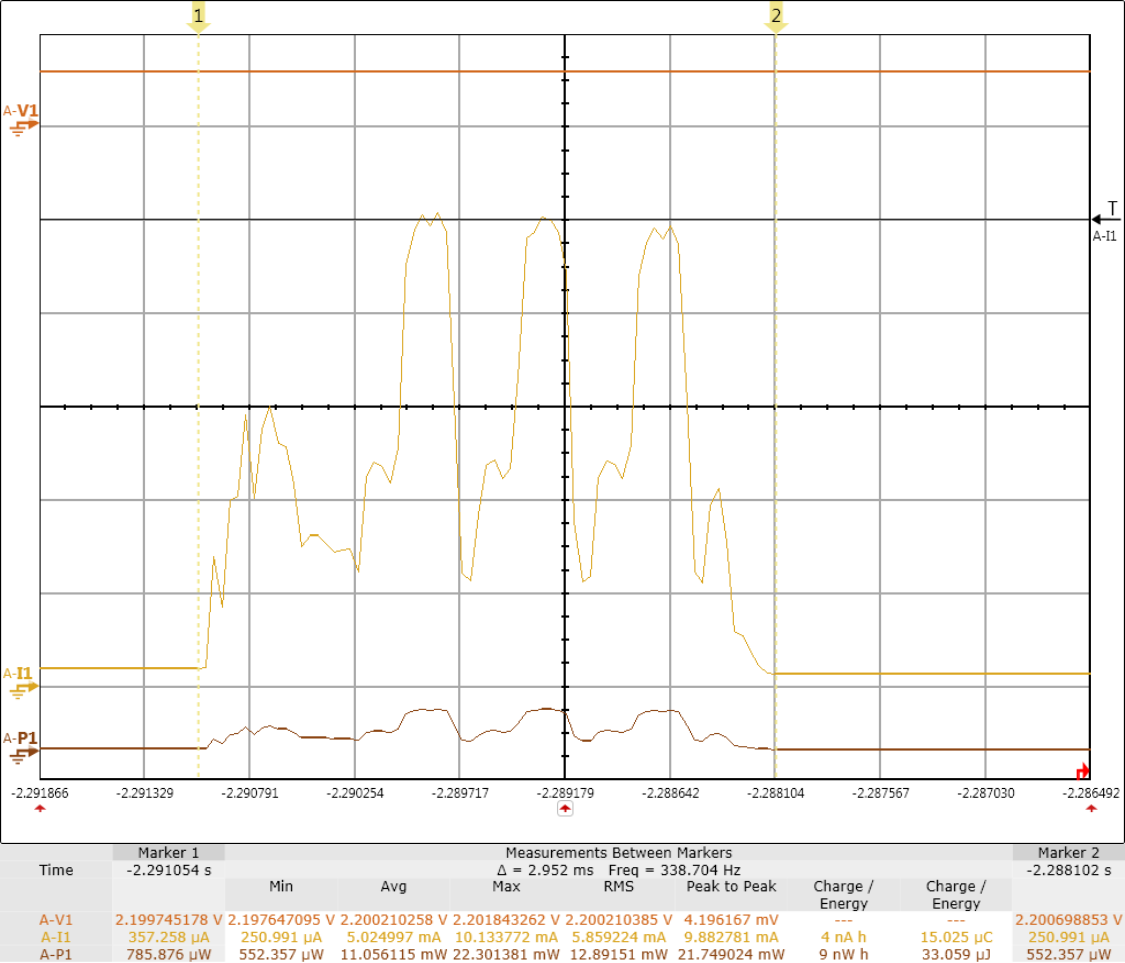
\includegraphics[scale=1]{3Vorgehen/imag/v0Send33uJ.png} 
    \caption{Minimalster Energieverbrauch: 3 BLE Pakte über Advertising Mode senden}
    \label{BLE_send}
\end{figure}

Um einen Anhaltspunkt über den Energieverbrauch des Sensortags zu erhalten, wurde 3 BLE-Pakete im Advertsing Mode per Knopfdruck gesendet (siehe Abbildung \ref{BLE_send}). Dies entspricht der Messung zur Sensortagversion V0. Nach der Weiterentwicklung des Programms, folgte die Messung V1, in der zusätzlich die GPIO ausgelesen werden. Dies ist für das Einlesen der Reed Switch-Impulse unumgänglich und für das Einlesen der Energy States vom 8500 sinnvoll. Die Version V2, erster Versuch mehr Sleep-Time einzubauen, scheiterete am Zusammenspiel des Timings der Radio- und GPIO-Interrupts. Das Neuaufsetzen des Programms half, sodass die Version V3 power-optimiert Geschwindigkeitspakete sendet. Die untenstehende Tabell stellt die ersten Energieresultate dar. Unterschieden wird zwischen dem Energieverbrauch für die Initialisierung und der Energie zum Senden von 3 BLE Paketen. Die Diskussion über Energieoptimierungen und die Deutung der Resultate finden sich in den Sitzungsprotokollen vom xxxxx - xxxx.
\todo{Sitzungsprotokolle Datum einsezten}

\subsubsection*{Messresultate nach Sensortag-Versionen}
\begin{tabbing}
    Version   \quad\= Datum     \quad\= Energie Init    \quad\=  Energie Senden \\[0.8ex]
    V0        \> 10.3.16        \> unbekannt            \> 33 $\mu$J \\
    V1        \> 16.3.16        \> 87 $\mu$J            \> 32 $\mu$J \\
    V3        \> 22.4.16        \> 40 $\mu$J            \> 29 $\mu$J \\
\end{tabbing}

Bei diesen Messungen werden die Sensoren noch nicht ausgelesen. Es zeigt sich, dass das Auslesen der Sensoren über I2C und das Warten, bis dass die Sensoren aufgestartet sind, viel mehr Energie verbraucht, als erwartet. Der Energieverbrauch des Auslesens nur eines Sensors (erste Priorität hat laut Aufgabenstellung der Drucksensor) ist ohne Optimierungsmassnahmen so gross, dass kein Senden der Daten mehr möglich ist. Die Speisung der Applikation bricht sofort zusammen (siehe Abbildung \ref{i2c_problem}).

\begin{figure}[ht]
    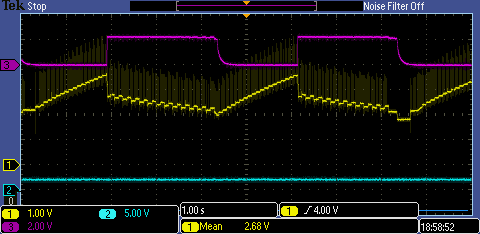
\includegraphics[scale=1]{3Vorgehen/imag/pic4VSUPbrichtEin.PNG} 
    \caption{Auslesen der Sensoren reisst Energie zusammen}
    \label{i2c_problem}
\end{figure}

Aus diesen Grund wurde die Power-Optimierung innerhalb des Programms zur zentralen Herausforderung in dieser Arbeit. Details darüber sind im nächsten Unterkapitel \ref{powerOptimierung} Power Management zusammengefasst. Neben dem konkreten Messen des Energieverbraus jedes Sensors auf dem Sensortag, folgt im Unterkapiteln \ref{energie senosortag}, ist auch der Energiegewinn an der Harvesterspule wichtig. Dies, weil sich in der Entwicklung des Prototypen zeigt, dass Energie durch die Hardwarschaltung selbst verloren geht. Dieses Messresultat folgt nun gleich, danach kommen die Energieergebnisse zu den Sensoren.

\subsubsection{Spule}



\subsubsection{Sensortag}
\label{energie senosortag} 


\paragraph{Nur Geschwindigkeit: Simple Harvester}

\paragraph{Alle drei Sensoren nacheinander: Advanced Harvester}

\paragraph{Nur Drucksensor}

\paragraph{Nur Temperatursensor}

\paragraph{Nur Feuchtigkeitssensor}




% x.2 ---------------------------------
\subsection{Energiekalkulation}
\label{v_e_kalkulation}

Der Energieverbrauch hängt von der Anzahl ausgelesener Sensoren ab (siehe \ref{v_messungen_sensortag}). Für die Bestückung der Kondensatoren wird vom schlechtesten  Fall, einer Geschwindigkeit von 10 km/h ausgegangen. Die Grundlagen zur Energiekalkulation sind im Theorieteil \ref{th_energiebilanz} abgebildet. Hier werden die Kondensatoren berechnet.



Die Energie der Quelle [$\bar{E_{HRV}} $] muss ausreichen für das Versenden der Datenpakte über Bluetooth smart [$\bar{E_{BLE}}$].

\[\bar{E_{HRV}} \ge \bar{E_{BLE}}  \]



\[\bar{E_{HRV}} = \bar{P} * t \ge \bar{E_{BLE}}  \]
\[\bar{P_{10km/h}} * t = 11 * 10^{-3}  \]
\[74.4 * 10^{-6} * t = 11 * 10^{-3}   \]
\[t = 147 s  \]

\[\bar{E_{HRV}} = \bar{P} * t \ge \bar{E_{BLE}}  \]
\[\bar{P_{10km/h}} * t = 11 * 10^{-3}  \]
\[74.4 * 10^{-6} * t = 11 * 10^{-3}   \]
\[t = 147 s  \]


\subsubsection{MPP einstellen}

\todo{Messprotokolle eintrage}

Das Ziel der Entwicklung ist, dass bei einer Geschwindigkeit von 10 km/h genug Enerige zum Senden eines BLE-Pakets zur Verfügung steht. Während der Entwicklung des Harvesters wurde die Leistungskurve öfters aufgenommen (siehe Anhang \ref{uebersicht_messprotokolle}, xxx,yyy, zz). Wie im Theorieteil erklärt \ref{harv_diff} unterscheidet sich das Leistungsmaximum nach Geschwindigkeit. Weil das Ziel ein funktionstüchtiger Prototyp bei 10 km/h ist, bezieht sich das Einstellen nur auf diese Wert.  

 
\subsubsection*{MPP-Ratio bei 10 km/h gemäss Messprotokollen}
\begin{tabbing}
    Datum       \quad\= Leistungmaximum    \quad\= MPP-Ratio\\[0.8ex]
    30. März    \> 12 $\mu$W        \> 43.23\thinspace\% \\
    xx          \> xx $\mu$W        \> xx\thinspace\%\\
    resultat    \> 21.87  $\mu$W    \> 24.87\thinspace\%\\
\end{tabbing}

Es zeigt sich, dass das Leistungsmaximum unterhalb von 50\thinspace\% liegt. Bedauerlich ist, dass durch die Energieoptimierung sich die Stelle des Leistungsmaximums Richtung Leerlauf verschiebt. In der Umsetzung mit dem EM8500-Chip ergibt sich das Problem, dass nur Konfigurationen von MPPT-Ratios von 50 - 80\thinspace\% erlaubt sind (siehe Tabelle unten).  Die Einstellungen der tieferen MPP-Ratio sind zudem gröber. Dies, weil der EM8500-Chip für Harvester vom Typ TEG (mit einem MPP konstant bei 50\thinspace\%) und Solarzelle konzipiert ist und die MPPT-Ratio für diese zwei Anwendungen genau in diesem Range liegen. In unserem Fall ist dieser vorgegebene Range nicht ideal. Da beim energiekritischen Zustand bei 10 km/h die Ratio deutlich unter 50\thinspace\%. Die Vorgänger wählten in ihren Einstellungen eine MPPT-Ratio von 88\thinspace\%. Die Vermutung liegt nahe, dass keine Leistungskurve des Harvesters im Voraus aufgenommen wurde.


\subsubsection*{MPPT-Ratio Einstellungen EM8500}
\begin{tabbing}
    Registerwert   \quad\= MPPT-Ratio    \\[0.8ex]
    0x00           \> 50\thinspace\% \\
    0x01           \> 60\thinspace\%\\
    0x02           \> 67\thinspace\%\\
    0x03           \> 71\thinspace\%\\
    0x04           \> 75\thinspace\%\\
    0x05           \> 78\thinspace\%\\
    0x06           \> 80\thinspace\% \\
    0x07           \> 82\thinspace\%\\
    0x08           \> 83\thinspace\%\\
    0x09           \> 85\thinspace\%\\
    0x0A           \> 86\thinspace\% \\
    0x0B           \> 87\thinspace\%\\
    0x0C           \> 88\thinspace\%\\
\end{tabbing}

\todo{Sitzungsprotokoll Datum}
Im ersten Versucht wird das Register auf das Minimum (50\thinspace\%) eingestellt (siehe Sitzungsprotokoll YYYY). Die Messung ergab, dass bei 10 km/h das EM-Board nicht gespiesen wird. So luden sich weder der STS noch der LTS auf. Der Grund ist, dass der optimale Leistungsbezug bei 50\thinspace\% liegt, das Leistungsmaximum aber später. So entstand beim Regeln auf den optimalen Leistungsbezug der Umstand, dass dort nur 0.2 V produziert werden. Dieser Spannungswert ist zu tief, der EM-Chip beginnt nicht zu arbeiten. Betreibt man den Harvester nicht am optimalen Punkt, sondern bei einer MPPT-Ratio von 60\thinspace\%, so wird eine Eingangsspannung von 0.3 V produziert und EM8500 beginnt zu arbeiten.




% x.3 -------------------------------------
\subsection{Einstellen der Schwellwerte}
\label{v_schwellwerte}

Einstellungen Chip mit Ziel LTS für 10 km/ mit  MPP
Im Theorieteil kurz beschrieben.


\subsubsection*{Tabelle Finale Konfiguration Schwellwerte }
\begin{tabbing}
    Register .............\quad\= Spannungswert \\[0.8ex]
    v\_bat\_max\_hi       \> 3.9 V \\
    v\_bat\_max\_lo       \> 3.8 V \\
    v\_bat\_min\_hi\_dis  \> 3.6 V \\
    v\_bat\_min\_hi\_con  \> 2.2 V \\
    v\_bat\_min\_lo       \> 2.0 V \\
    v\_appl\_max\_hi      \> 3.8 V \\
    v\_appl\_max\_lo      \> 3.7 V \\   
\end{tabbing}

Zeigen, dass Bat bin lo höher gehen muss.

Zeigen, dass max STS genügt. Kompromiss zu 

% x.4 -----------------------------------------
\subsection{Energiezustand des Systems}
\label{v_energiezustand}

Die letzte der vier Aufgaben aus der Optimierungsliste nach der Inbetriebnahme (siehe Unterkapitel \ref{optimierung}) ist das variable Anpassen des BLE-Paketsendens aufgrund des Energiezustandes. Im ersten Unterkapitel \ref{def_zustaende} wird das Einteilen des Systems in Energiezustände beschrieben, dann drei Implementierungen, wobei der letzte Ansatz im Prototyp angewendet wurde. 

\subsubsection{Definition von Energiezuständen}
\label{def_zustaende} 


Da die produzierter Energie von der Fahrgeschwindigkeit abhängt, wird das Energiesystem in drei Zustände eingeteilt, die von der Geschwindigkeit abhängen:

\subsubsection*{Energiezustände aufgrund der Geschwindigkeit}
\begin{tabbing}
   0 - 15 km/h      \quad\= LOW\_ENERGY   \\[0.8ex]
   15 - 25 km/h      \> MIDDLE\_ENERGY \\
   $>$ als 25 km/h   \> HIGH\_ENERGY\\
    
\end{tabbing}

Was in den eingelnen Energiezuständen gemacht wird:

Bild








 4---------------------------------------------------------------------------
\section{Power Management}
\label{powerOptimierung}

Aufgrund von Messungen -> Codeoptimierung


%... noch zu schreiben ....
%Üblicherweise wird das RTOS-Betriebssystem von TI für Low Power Applikationen benutzt. 


%(Die Low-Power Programmbeispiele von TI basieren auf RTOS, ebenso die Dokumentation zu Low Power Applikationen, was zu viel Energie verbraucht (korrekt, wie belegen?). )


%Problem: So gehört zu jedem Aufwecken einer Peripherie, der Parallele Schlafmodus, bis dass die Peripherie gestartet ist. (Dies gilt auch für die Sensoren.) Zu lange warten: braucht Energie.
%
%Sleep konkret: Power Banks abschalten:\\
%Power Domains zeigen
%
%Schwierigkeit Interrupt and Events !!
%
%Bild: Energie-Langzeitmessung BLE versenden\\
%Beschriften mit aktiv und standby modus
%
%
%Gearbeitet wird mit einem Cortex M3 von TI.\\ 
%Grundsätzlich basieren die Bsp. auf RTOS. Wenige für PowerManagement. Das Powermanagement ohne Betriessystem. Wir verwenden dies, weil (gemäss Erfahrungswerte Praxis) mit Betriebsystem mehr Energie braucht).


\begin{figure}
  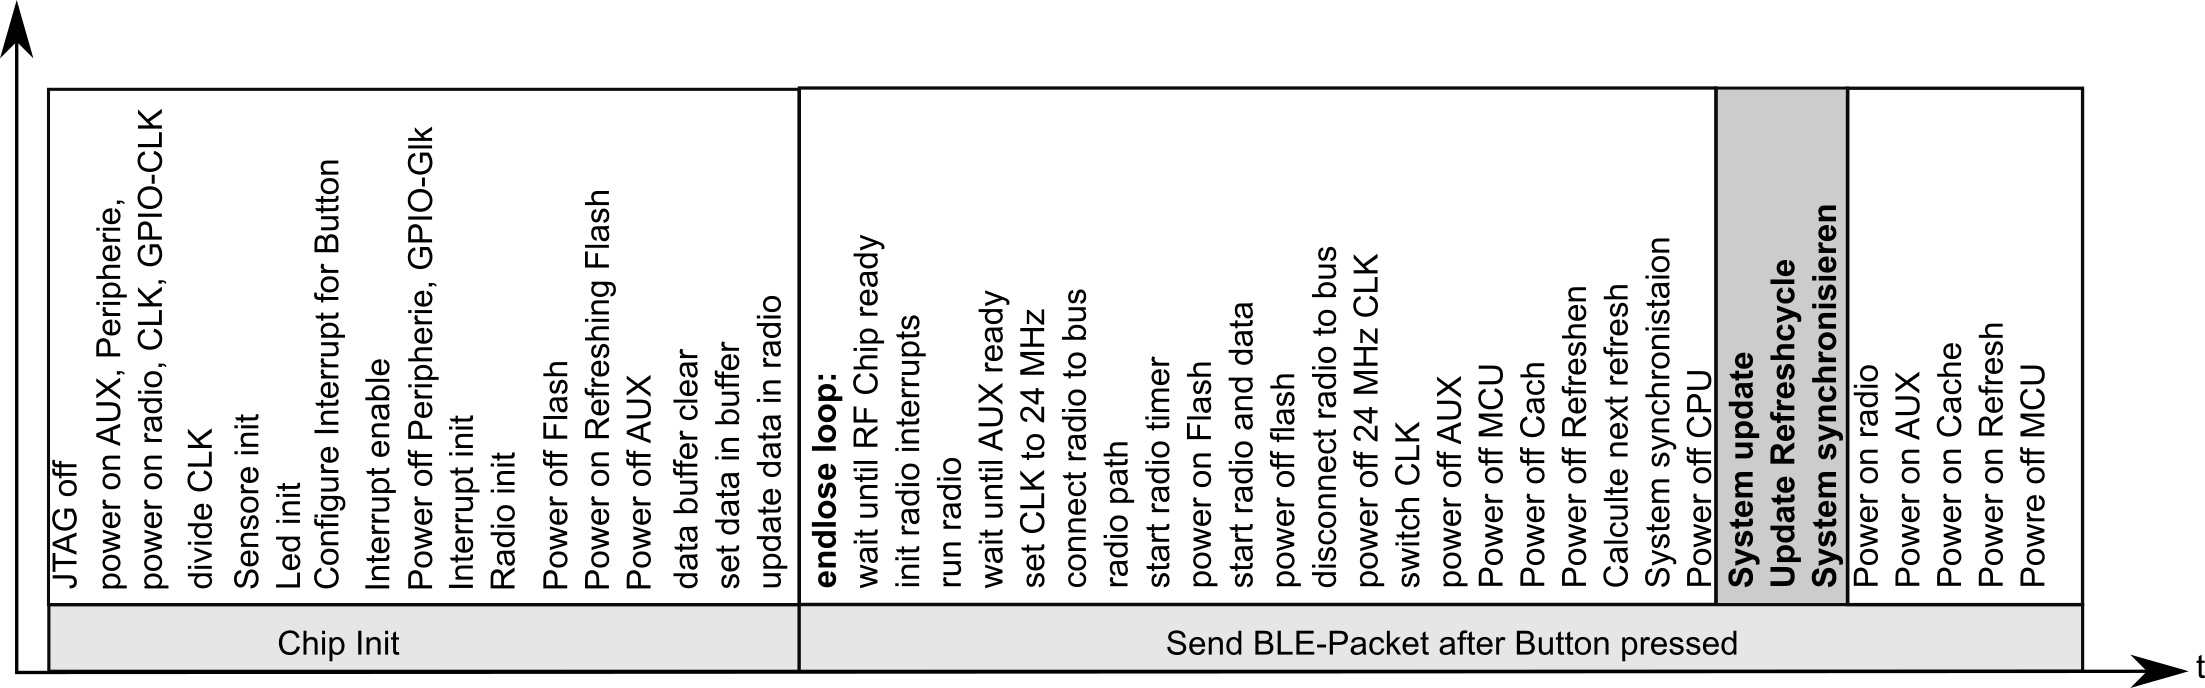
\includegraphics[width=1.0\textwidth]{../ressources/SimpleLink/V0Sendeablauf.png}
  \caption{Prozessablauf V0}
\end{figure}




% 5 ---------------------------------------------------------------------------
\section{Applikationsentwicklung}

\subsection{Aufbau der App}

\subsubsection{BLE empfangen und filtern}

\subsection{Grundeinstellungen}

\subsection{Tachometer einbauen}

\subsection{Modularer Aufbau}

Die Applikationsentwicklung basiet auf einer modularen Struktur.  Dadurch wird eine Weiterentwicklung der Applikation ohne Probleme möglich. Ebenfalls wurde beachtet, dass die Applikation sogar in andere Sprachen übersetzt werden können muss, dafür wurden alle Texte, die ersichtlich sind in einem File aufgenommen und können zentral abgeändert werden, ohne einen Eingriff in den aktuellen Code.


Mit Android Version xx.

--- alter Text --- 

\subsection{Aufbau der App}

Welche Aktion zu welchem Display gehört (Überblick Gesamtsystem)


\subsection{Implementierte Aktionen}
Geräteauswahl
Kalibrierung
Geschwindigkeitsberechnung
Sensordaten ausgeben (was mit welcher Genauigkeit)

\subsection{BLE Empfangen}

Aufbau des Datenpakets: 
LEN, UUID, ...







\chapter{Resultate}
\label{ch_resultat}

(In den Messprotokollen \todo{Auflisten der Messprotokolle} auf der CD sind diverse Energiemessungen dokumentiert.
 
\section{Harvesterschaltung}

\subsection{Leistung am Harvesterausgang}

Essentiell ist es zu wissen, wie viel Energie von der Harvesterschaltung zur Verfügung gestellt wird. Die Leistungskurve gibt Aufschluss wie viel Leistung bei verschiedenen Geschwindigkeiten gewonnen werden kann. Bei der eingetragenen Leistung handelt es sich um die maximal zur Verfügung stehende Leistung, also die Leistung im MPP. In Abbildung \ref{mpp_resultat_harvester} ist ersichtlich, dass die maximale Leistung mit erhöhen der Geschwindigkeit zunimmt.

\begin{figure}[ht]
    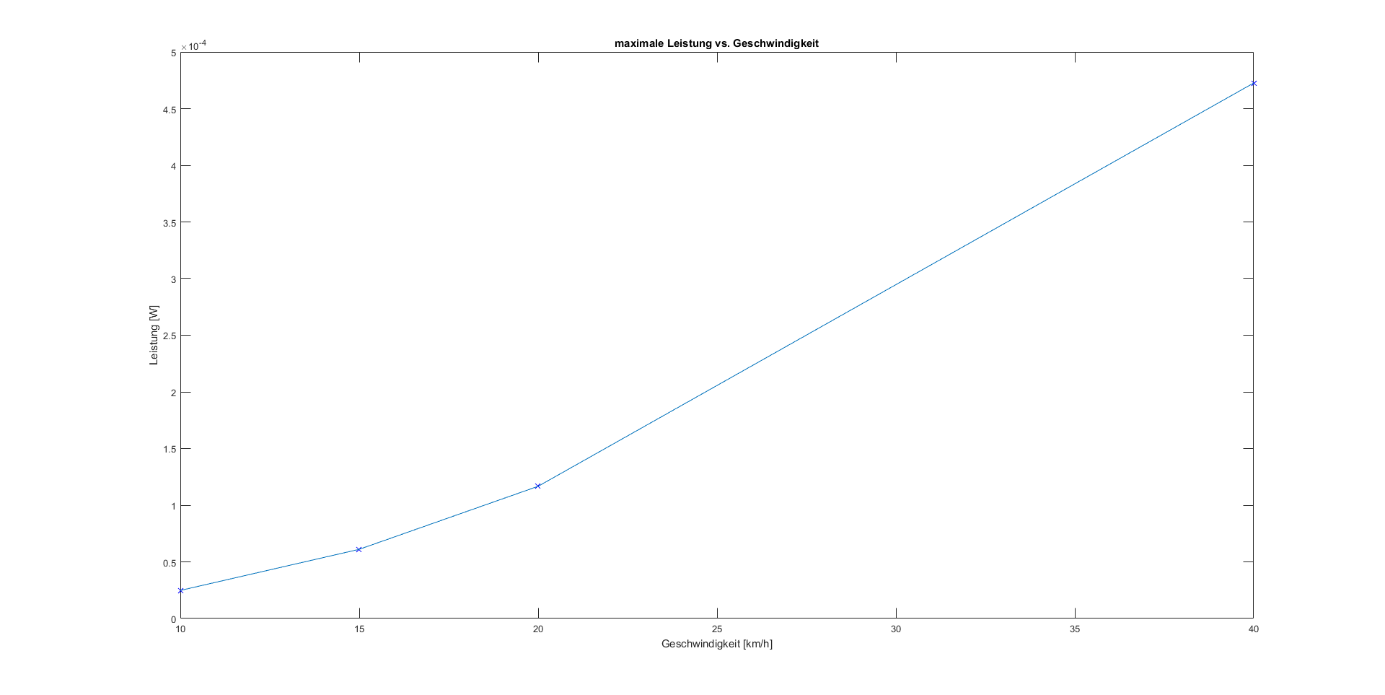
\includegraphics[width=0.5\textwidth]{4Resultate/imag/ResultatLeistungGeschwindigkeit.png} 
    \caption{Maximale Leistung vs. Geschwindigkeit}
    \label{mpp_resultat_harvester}
\end{figure}

\subsection{Verhalten des Harvesterausgangs}
Ein wichtiger Aspekt ist das reelle Verhalten des Harvesters bei Belastung mit dem EM-Chip. Der EM-Chip regelt den Eingang, bzw. den Ausgang des Harvesters, indem der Eingangswiderstand verändert wird. Somit soll der MPP erreicht werden, damit die Leistung immer maximal ist. Die Abbildung \ref{resultat_Harvester_Spannung} zeigt den Verlauf der Spannung am Eingang des EM-Chips über längere Zeit. Die Spannung wird auf ein stabiles Level geregelt und somit kann eine relativ konstante Leistung aufgenommen werden. Weitere Messungen und Werte können aus dem Messprotokoll \todo{Name heraussuchen} entnommen werden.

\begin{figure}[ht]
    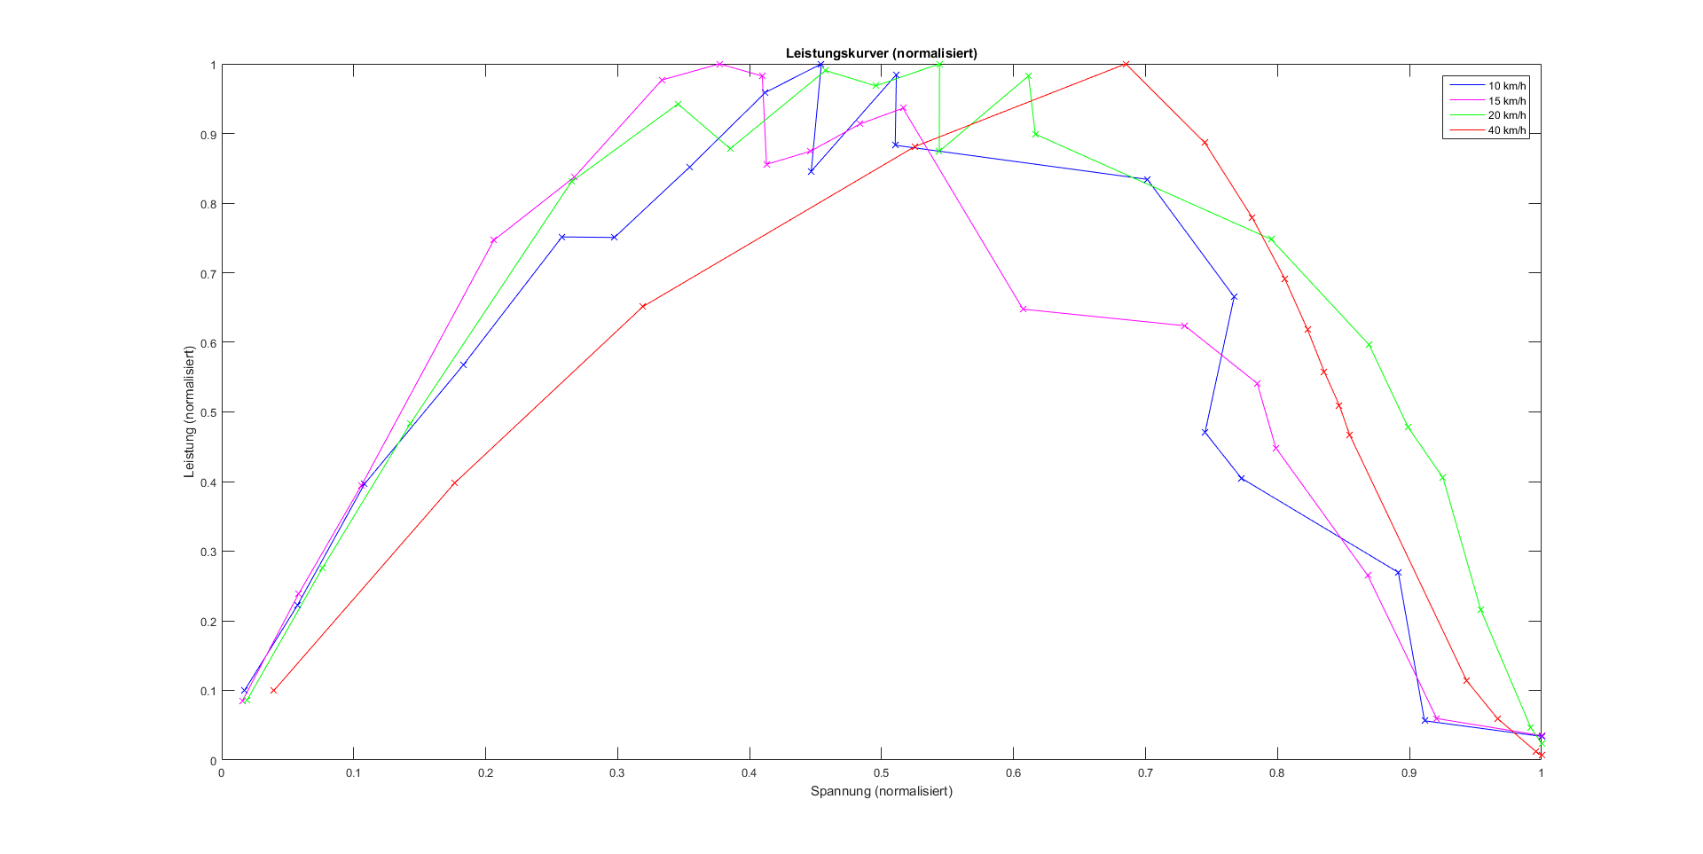
\includegraphics[width=0.5\textwidth]{4Resultate/imag/MPPHarvester.png} 
    \caption{Leistungskurve (normalisiert) }
    \label{resultat_Harvester_Spannung}
\end{figure}


\subsection{Energie am EM-Chipausgang}

Die Energie, welche vom EM-Chip abgegeben wird, steigt mit der Geschwindigkeit. Hier wurde die Energie von einem Puls gemessen, d.h. vom Einschalten von VSUP bis zur Abschaltung von VSUP. Nach diesem Puls wird keine Energie mehr abgegeben, bis zum nächsten Puls.

\begin{figure}[ht]
    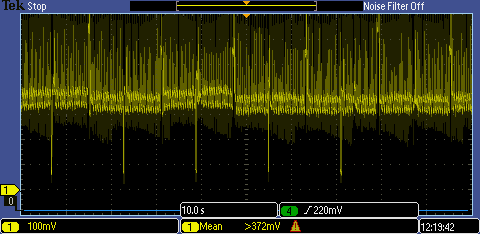
\includegraphics[width=0.5\textwidth]{4Resultate/imag/SpannungVCC.png} 
    \caption{Spannung VCC bei 15 km/h}
    \label{resutat_emchip_spannung}
\end{figure}


\subsection{Wirkungsgrad des Prototypen}

Interessant ist die Betrachtung des Wirkungsgrades des EM-Chips. In der nachfolgenden Tabelle sind die Leistungen aufgezeichnet, welche mit den aktuellen Einstellungen des EM-Chips anliegen.

\subsubsection*{Tabelle Leistung und Wirkungsgrad }
\begin{tabbing}
    Geschwindigkeit \quad\= Leistung Harvester \quad\= Leistung EM8500\_out \quad\= Wirkungsgrad\\[0.8ex]
    10 km/h  \> 21.87  $\mu$W \> 5.44   $\mu$W \> 24.87\thinspace\%  \\
    15 km/h  \> 57.19  $\mu$W \> 20.91  $\mu$W \> 36.56\thinspace\%  \\
    20 km/h> \> 114.67 $\mu$W \> 41.39  $\mu$W \> 36.09\thinspace\%  \\
    40 km/h> \> 416.29 $\mu$W \> 170.75 $\mu$W \> 41.01\thinspace\%  \\
\end{tabbing}   

Die Abbildung \ref{zsmEnergyGewinn} gibt einen Überblick, an welcher Stelle wie viel Energie vorhanden ist, bzw. zwischen welchen zwei Stellen wie viel Energie verloren ging.

\begin{figure}[ht]
    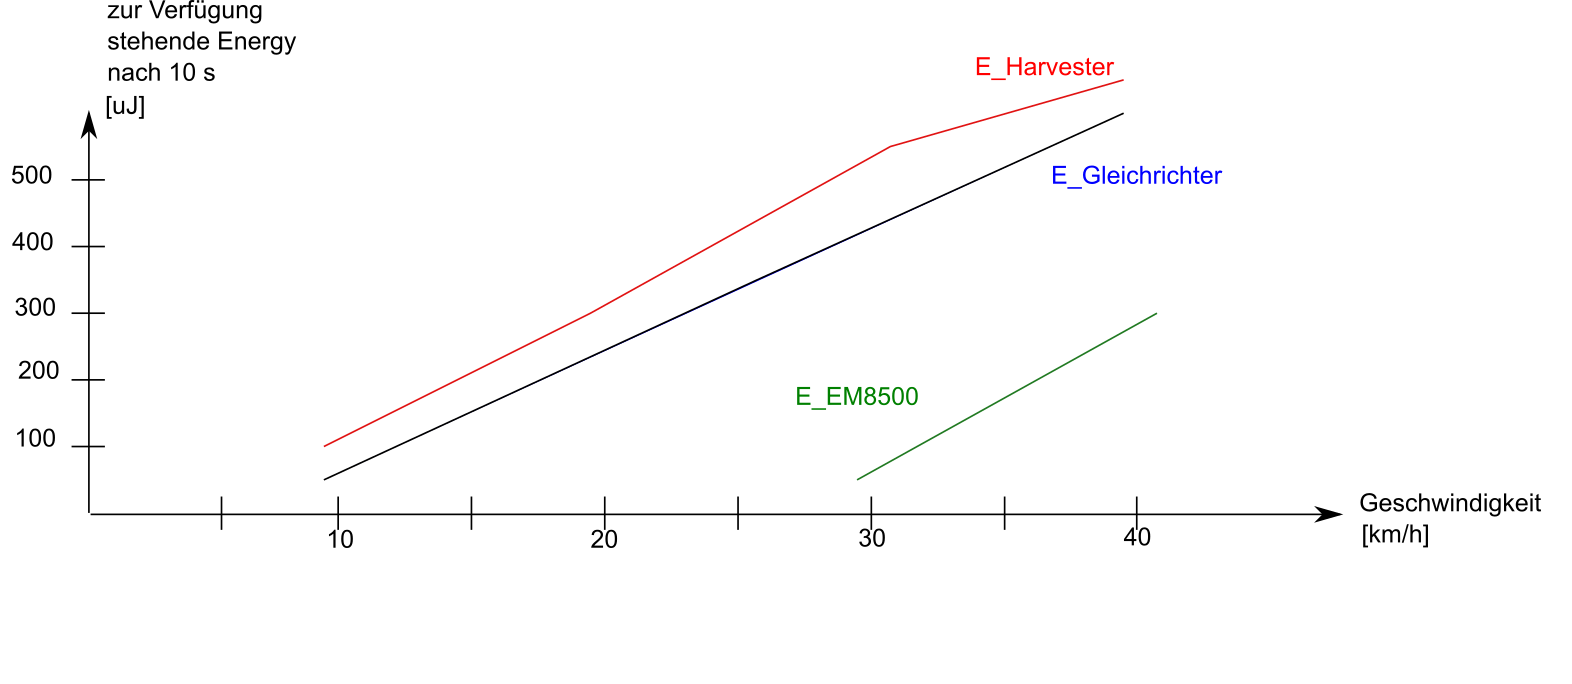
\includegraphics[width=1\textwidth]{4Resultate/imag/EnergyGewinnNachStelle.png} 
    \caption{Energiegewinn Zusammengefasst nach Stelle in der Schaltung}
    \label{zsmEnergyGewinn}
\end{figure}

Der Wirkungsgrad des EM8500 innerhalb des entwickelten Prototypen liegt bei 40 km/h  bei 41.01\thinspace\% und bei 10 km/h bei 24.87\thinspace\%.


\section{Energiemanagement}

%Beim Resultat spielt das Hard- und Softwaremanagment direkt ineinander, weshalb das Ergebnisse dieser zwei Aufgaben zusammen dargestellt werden.

Durch das korrekte Einstellen der Schwellwerte beim EM8500 (siehe Unterkapitel xxx) und die korrekten Ladewerte bei den Kondensatoren (siehe Unterkaptiel xxx), ist es möglich, dass sich der LTS-Kondensator bei einer Geschwindigkeit von YYY km/h lädt (siehe Abbildung xxx). Zudem entlädt sich LTS, sobald das Sensortag am Arbeiten ist (siehe Abbildung yyyy). Beim Energiemanagement ist es somit gelungen, die Schwellwerte und Kondensatorengrössen so einzustellen, dass die Funktionalitäten des EM8500-Chips voll ausgenutzt werden können.

\begin{figure}[ht]
    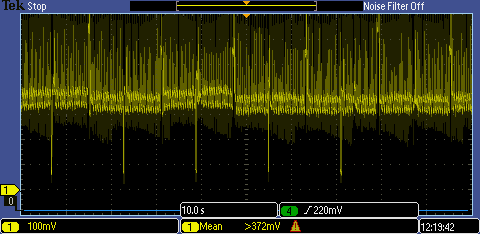
\includegraphics[width=0.1\textwidth]{4Resultate/imag/SpannungVCC.png} 
    \caption{STS und LTS laden sich}
\end{figure}

\begin{figure}[ht]
    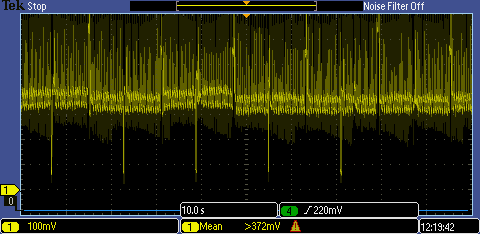
\includegraphics[width=0.1\textwidth]{4Resultate/imag/SpannungVCC.png} 
    \caption{LTS liefert Energie für die Arbeitspakete}
\end{figure}


\section{Powermanagement}

Durch ein gutes Powermanagement (siehe Unterkapitel xxx) wurde es möglich, die energiestarken Aufgaben in Teilen zu erledigen. Die Abbildung xxxx zeigt, das Aufteilen der Arbeitsschritte: Zuerst folgt das Init, dann folgt das Auslesen eines Sensors, dann das Senden des Sensors. Die Aufgaben wurden aufgeteilt, weil alle drei Schritte in einem zu viel Energie verbraucht hätte, sodass VSUP zusammengebrochen wäre.

\begin{figure}[ht]
    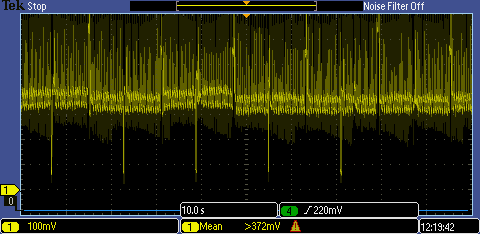
\includegraphics[width=0.1\textwidth]{4Resultate/imag/SpannungVCC.png} 
    \caption{Drei Arbeitspakte bis zum Senden der Daten }
    \label{blub}
\end{figure}

\todo{ ev. Grossaufnahme: BLE Energieverbrauch}

Die Abbildung \ref{resultat_E_Verbrauch_Verarbeitungsaufwand} zeigt den Energieverbrauch nach Verarbeitungsaufwand. Am wenigsten Energie benötigt das Berechnen der Geschwindigkeit über den RTC. Deutlich mehr Energie braucht das Auslesen der Sensor-Daten. Dies einerseits, weil die I2C-Kommunikation aufgebaut werden muss und weil die Sensoren eine gewisse Zeit brauchen, bis sie aktiv sind \todo{Aufwachzeit eines Sensors messen}. Die unterschiedlich verbrauchten Energiemengen entsprechen exakt den unterschiedlichen Startzeiten der Sensoren. 

\begin{figure}[ht]
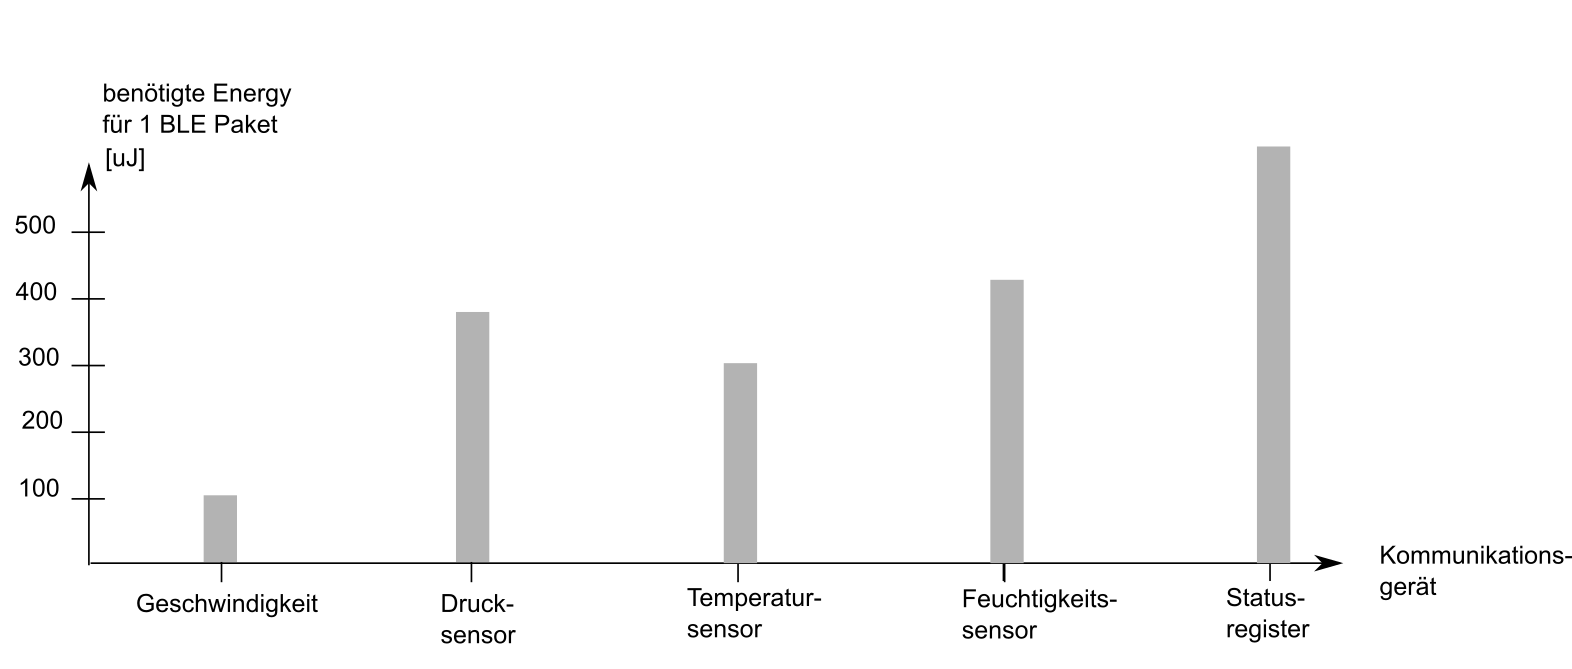
\includegraphics[width=1\textwidth]{4Resultate/imag/EnergyVerbrauchNachKommunikation.png} \label{resultat_E_Verbrauch_Verarbeitungsaufwand} 
\caption{Energieverbrauch gemäss Verarbeitungsaufwand für CPU}
\end{figure}

Kombiniert man den Energieverbrauch mit der zur Verfügung stehenden Energie am Ausgang nach dem EM8500-Chips, können (siehe Abbildung \ref{resultat_Zsm_Energy}) folgende Schlussfolgerungen gezogen werden:

\begin{enumerate}
    \item bla
    \item bla
    \item bla
    \item bla
\end{enumerate}

\begin{figure}[ht]
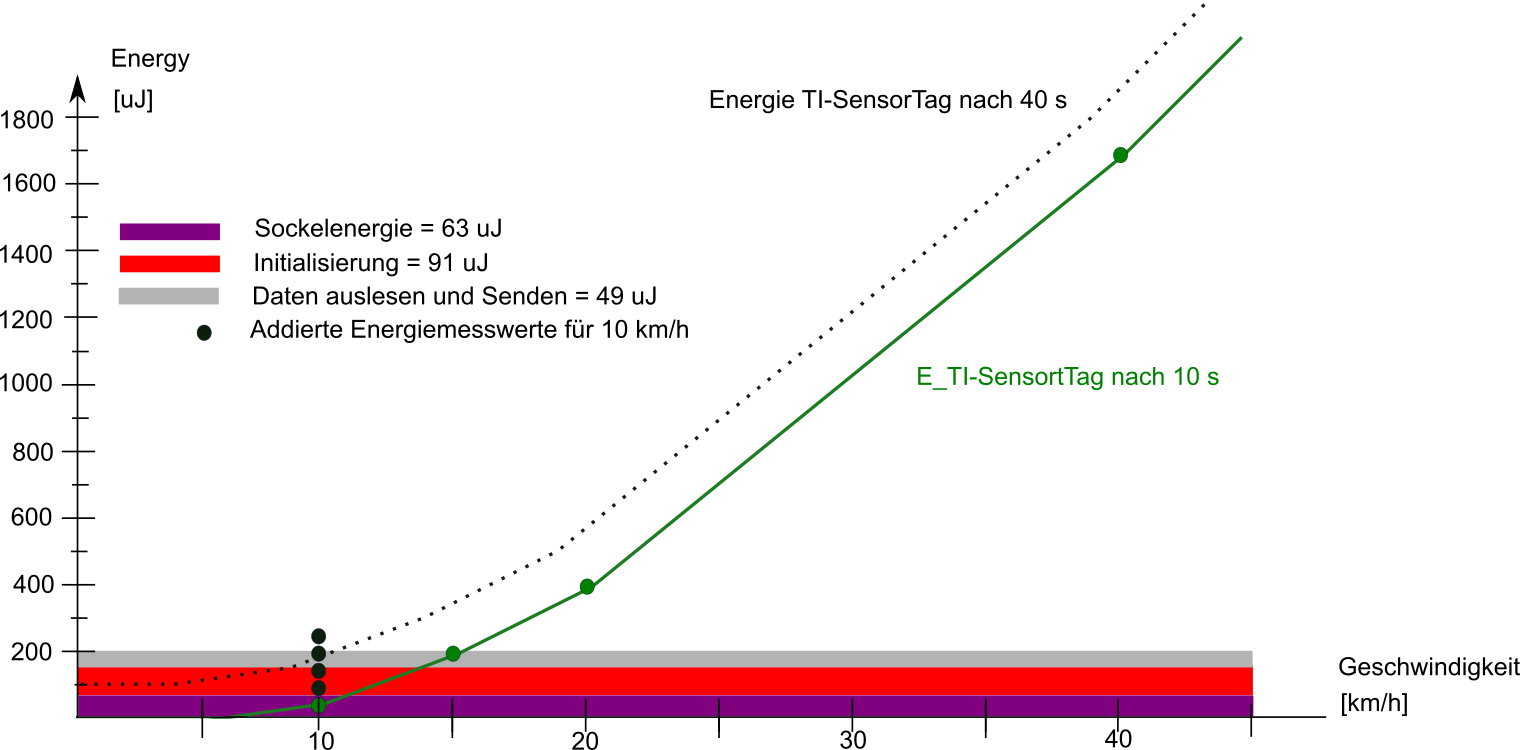
\includegraphics[width=1\textwidth]{4Resultate/imag/EnergyVerbrauchZusammenfassung.png}\label{resultat_Zsm_Energy} 
\caption{Energieverbrauch gemäss Verarbeitungsaufwand für CPU}
\end{figure}


\section{Ergebnisse BLE-Applikation}

Die Applikation ist bewusst einfach aufgebaut, um den Benutzer nicht zu verwirren. Der animierte Tachometer stellt dem User die aktuelle Geschwindigkeit schnell und übersichtlich dar. Weitergehende Funktionen sind durch prägnanete Namen selbsterklärend und der User sollte keine Mühe haben, die App ohne Lesen einer Anleitung zu verstehen.

\subsection{Applikationsstruktur}

Beim Öffnen der Applikation wird geprüft, ob Bluetooth aktiviert ist (siehe Abbildung \ref{permission}. Sollte Bluetooth nicht aktiviert sein, wird der User gefragt, ob Bluetooth aktiviert werden darf. Sollte der User die Aktivierung ablehnen schliesst sich die Applikation sofort.

\begin{figure}[ht]
    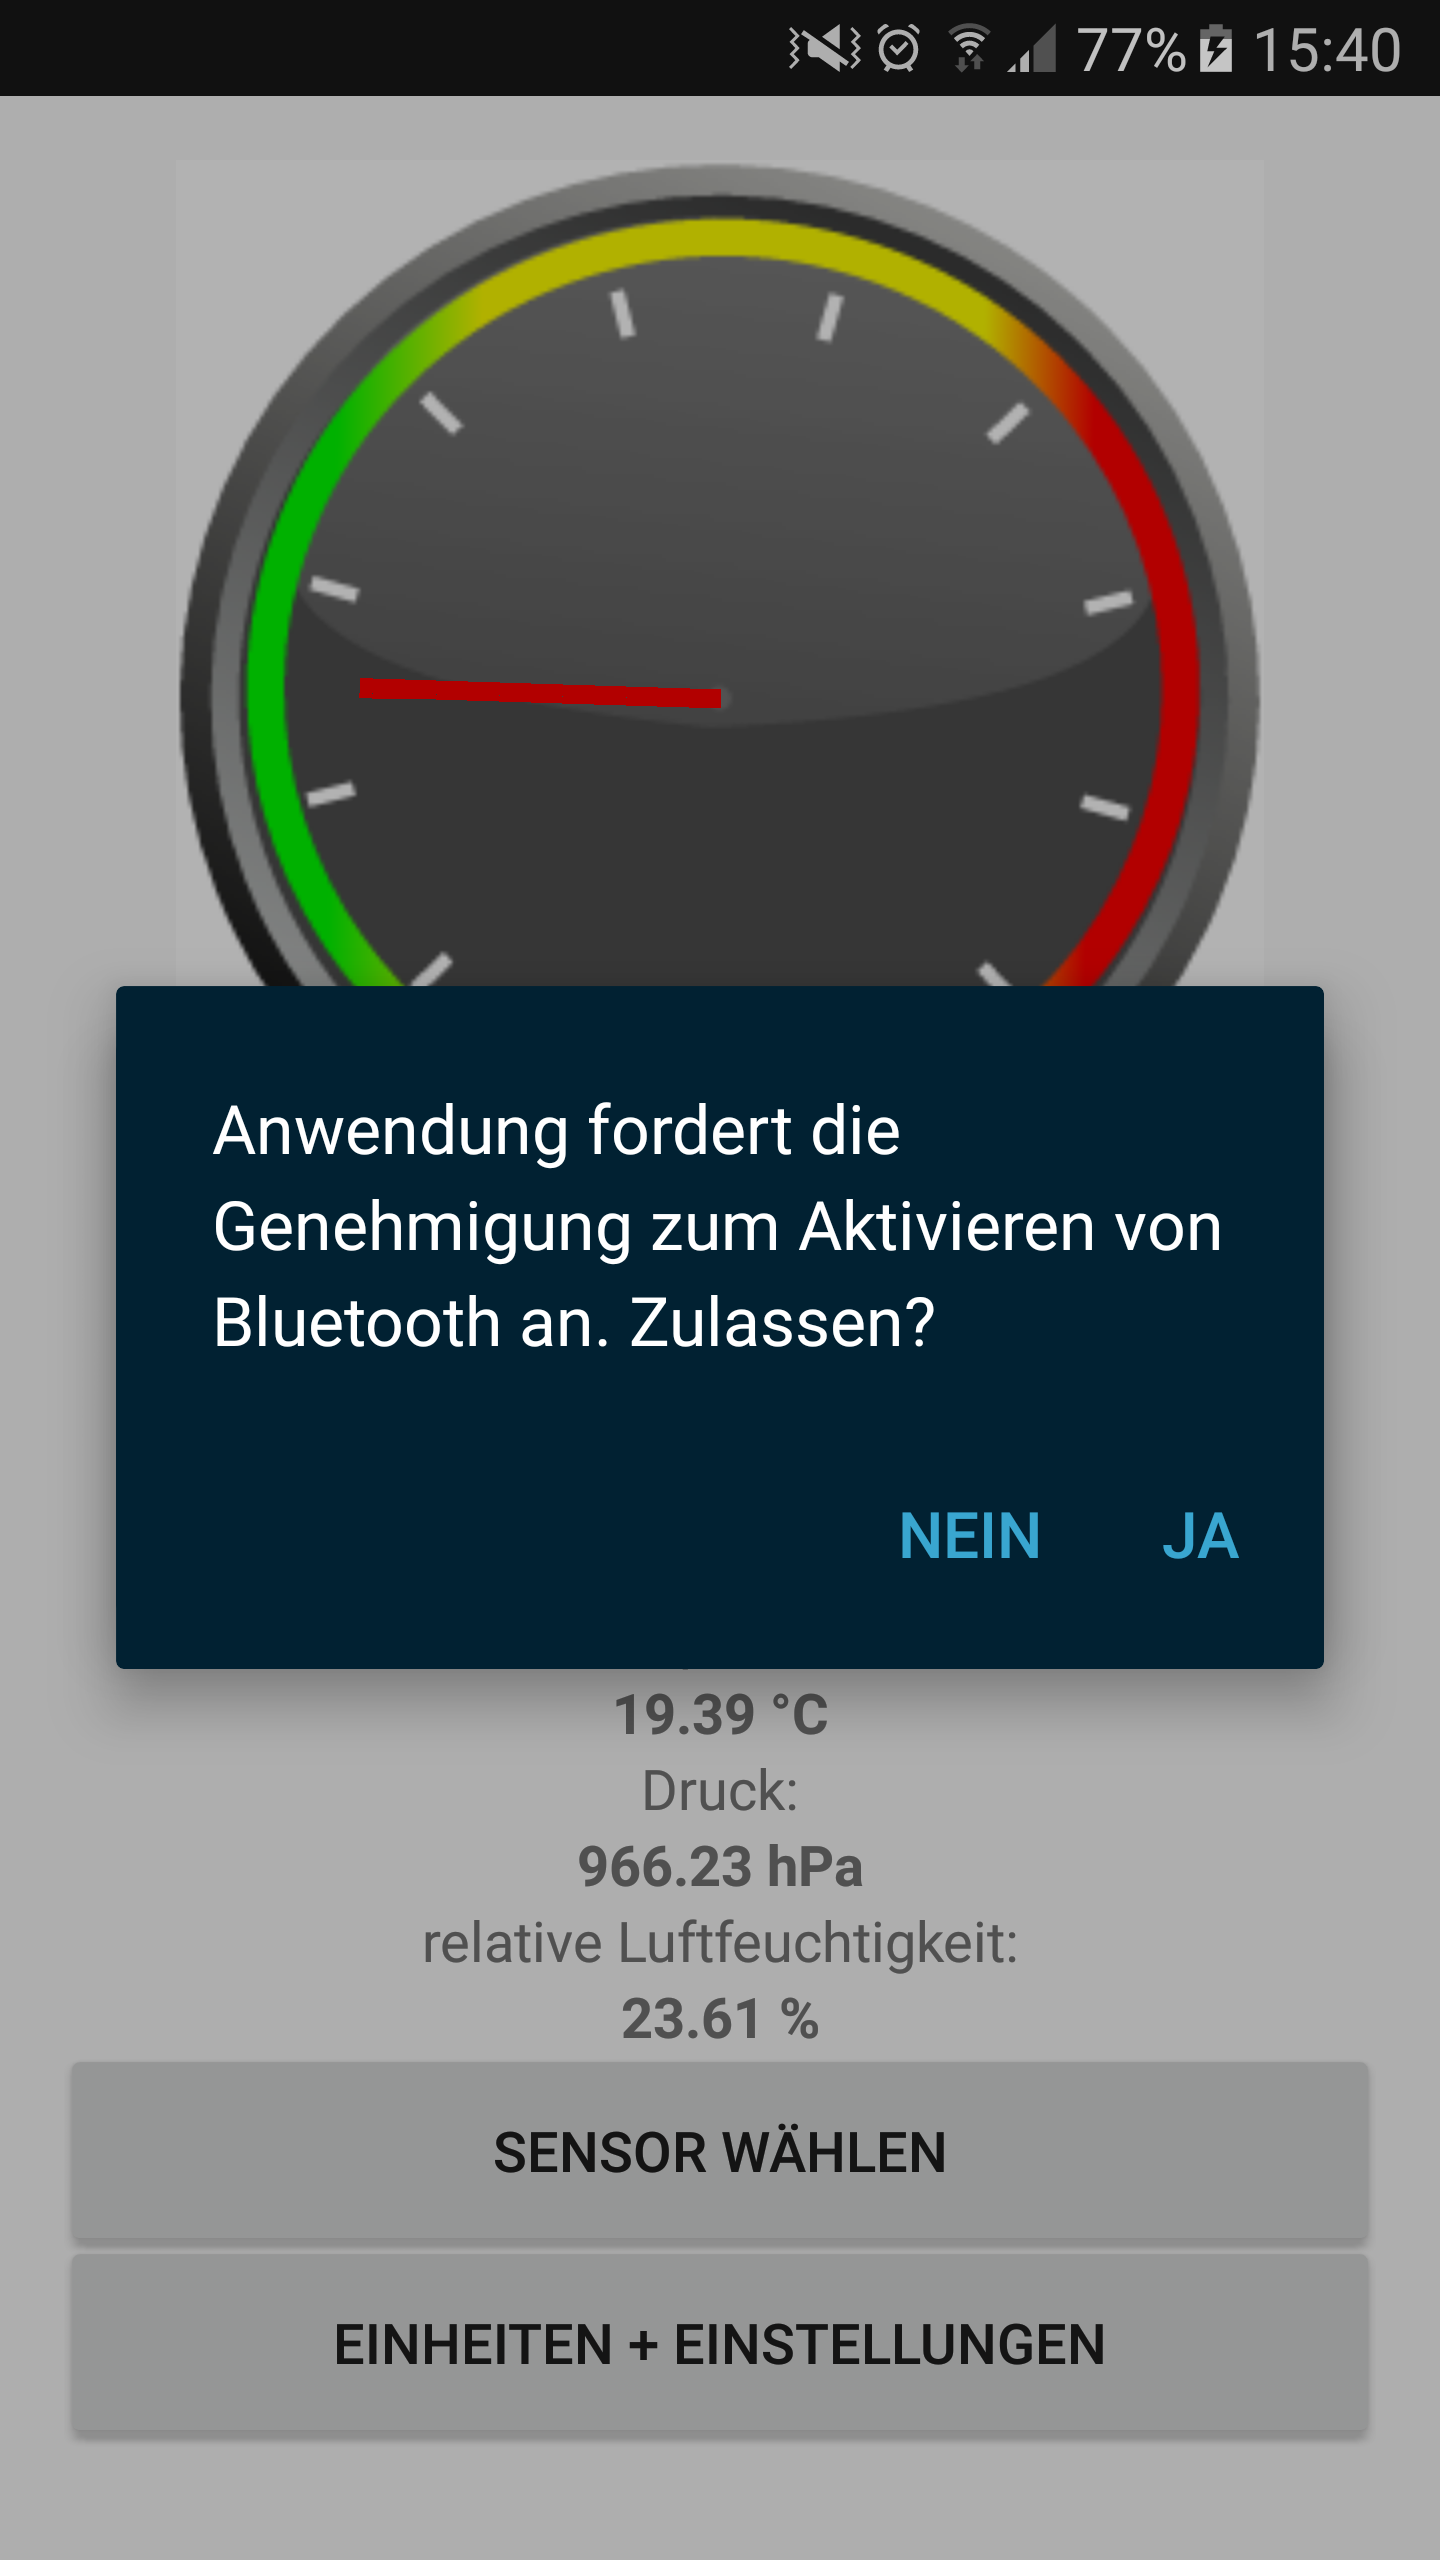
\includegraphics[width=0.5\textwidth]{4Resultate/imag/BLEBluetoothPermission.png} 
    \caption{Bluetooth Permission}
    \label{permission}
\end{figure}

Wird eine Verbund zu Bluetooth erlaubt, erscheint der Startbildschirm. Auf diesem befindet sich zentral der Tachometer (siehe Abbildung \ref{tacho}). Dieser zeigt Geschwindigkeiten von 0 – 90 km/h mit einer animierten Tachonadel an. Unterhalb des Tachometers werden die einzelnen Sensordaten angezeigt und im untersten Teil des Startbildschirms befinden sich zwei Buttons, über die man Einstellungen vornehmen kann. Die Kontextmenus zu diesen Einstellungen werden in den nächsten zwei Abbildungen \ref{sensorauswahl} und \ref{einheiten} ersichtlich. 

\begin{figure}[ht]
    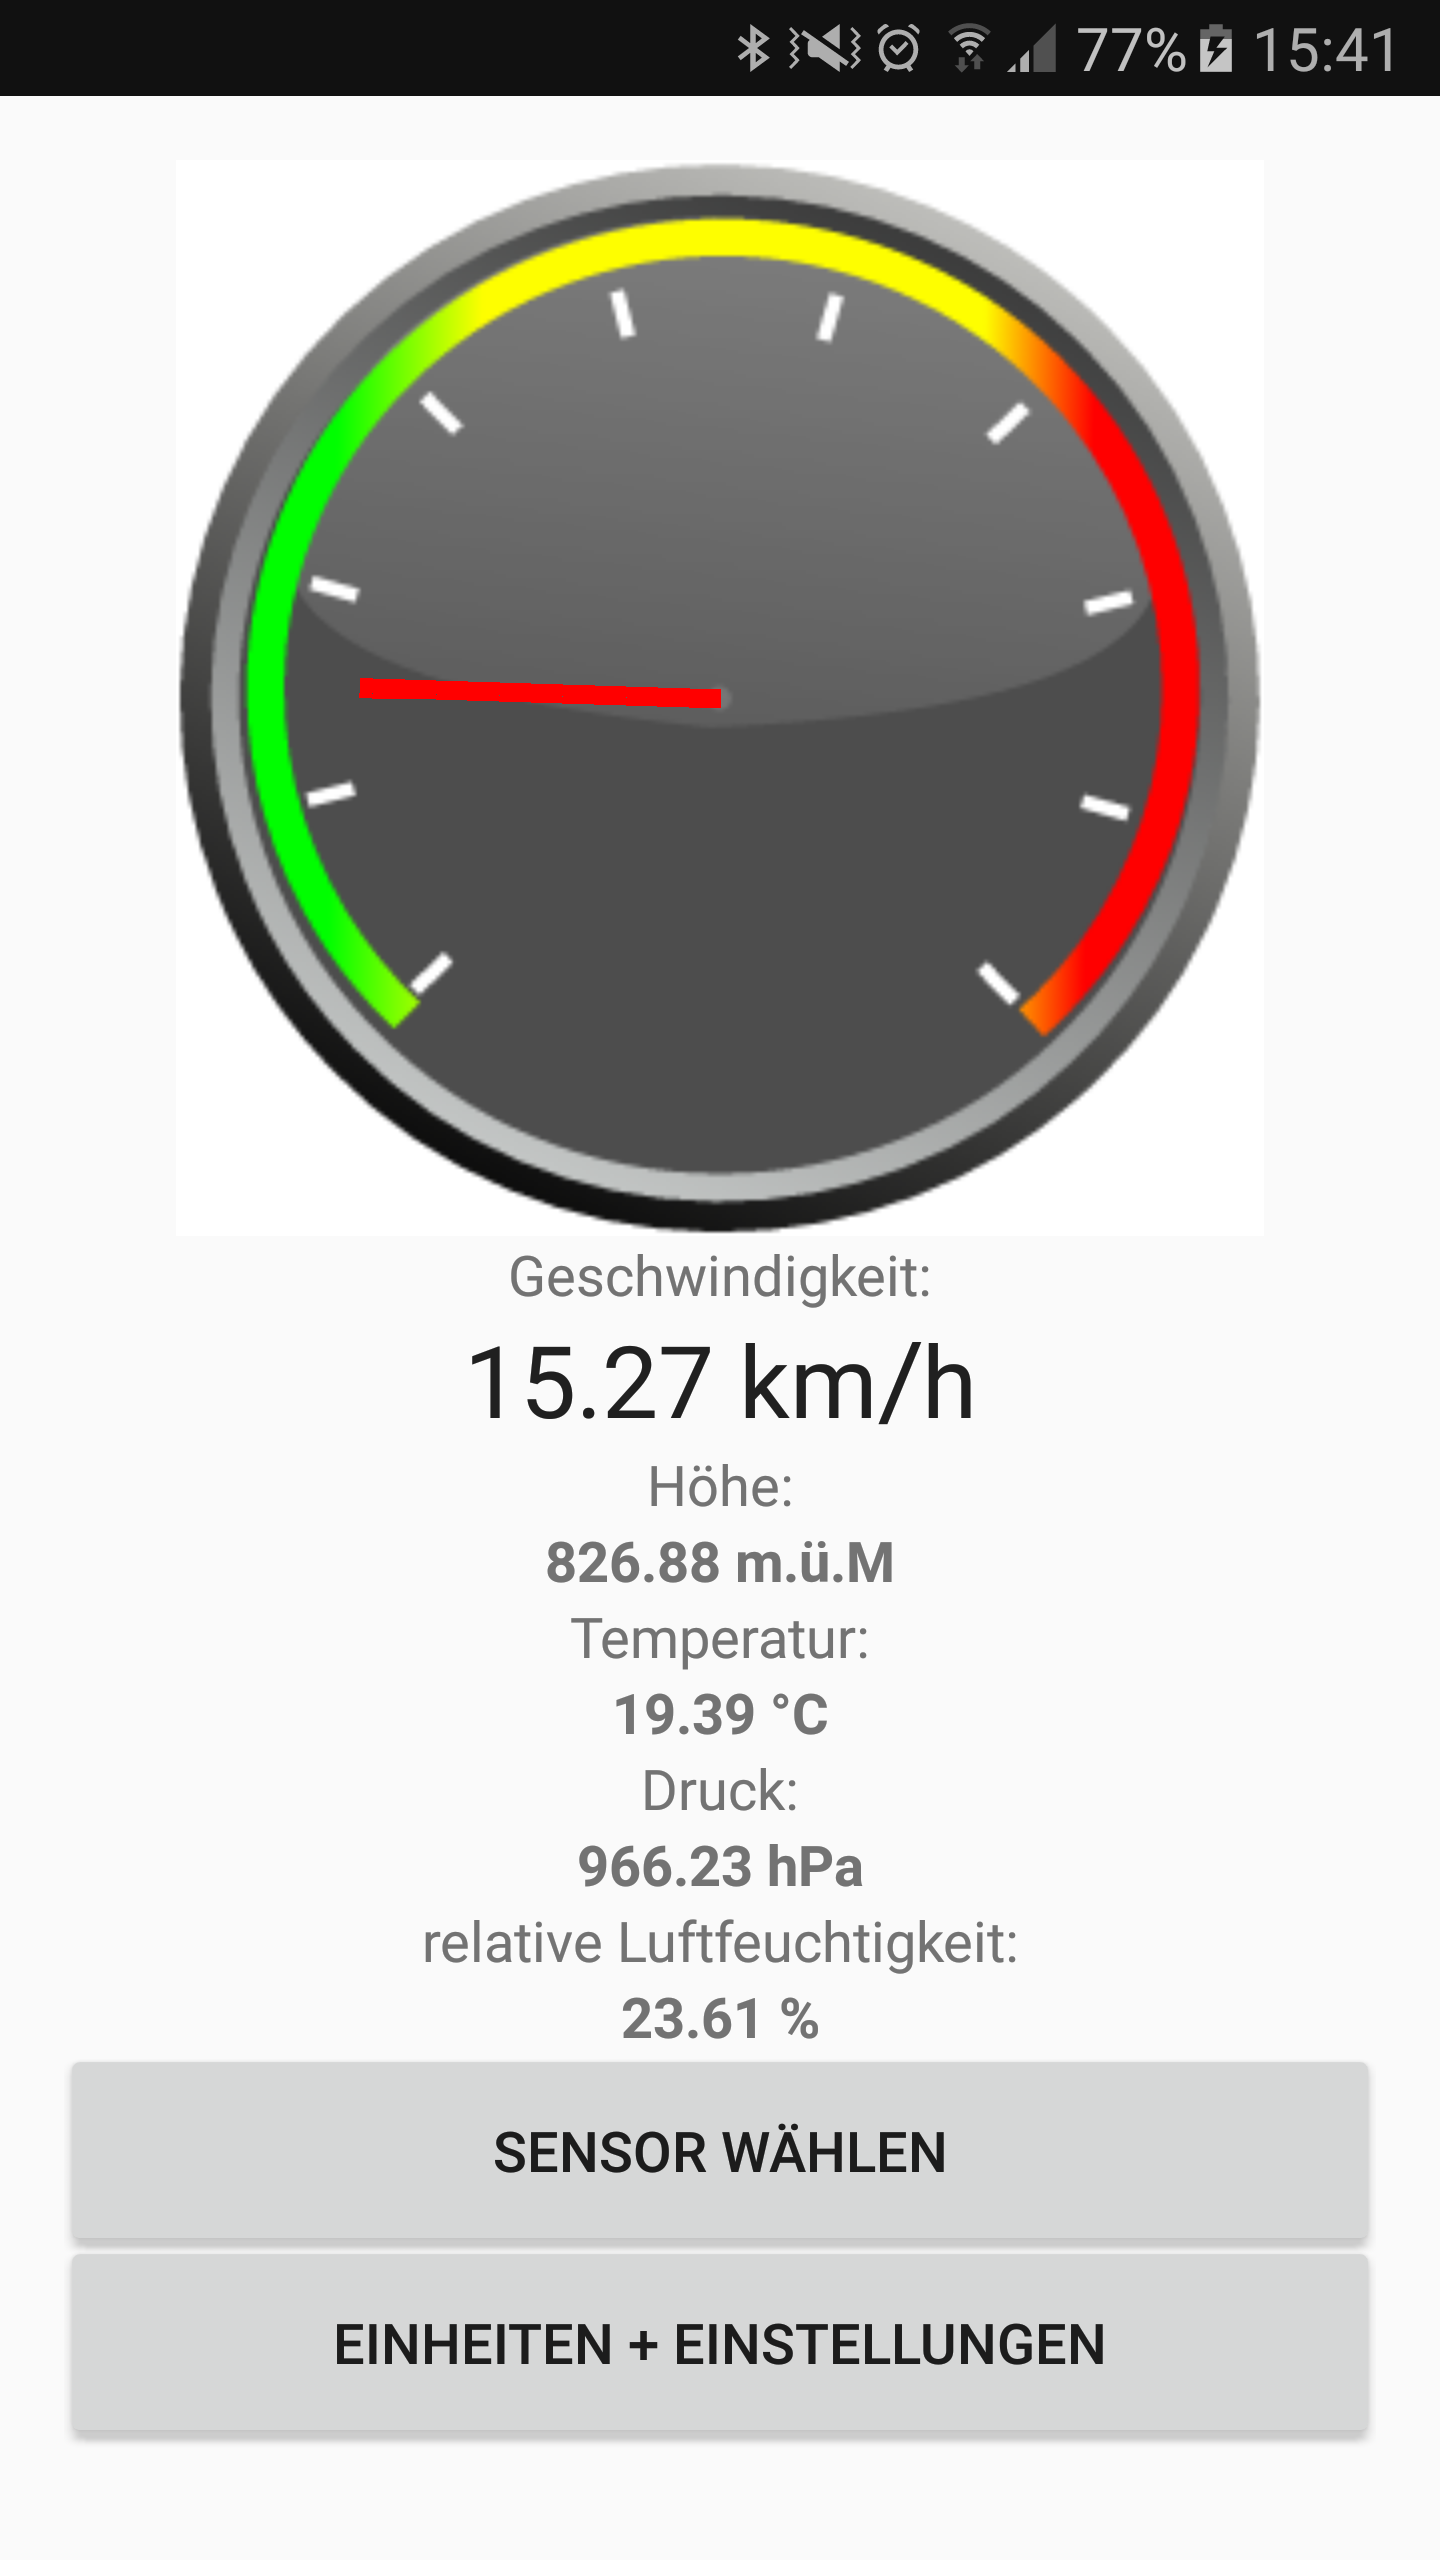
\includegraphics[width=0.5\textwidth]{4Resultate/imag/APPHomeScreen.png} 
    \caption{Startbildschirm der Applikation}
    \label{tacho}
\end{figure}

Wählt man auf dem Startbildschirm "Sensor wählen", \todo{ev. besser: Sensorboard wählen} erscheint ein neuer Bildschirm. Auf diesem erscheinen nur die aktiven Bluetooth Geräte mit dem implementierten Prototypen-Filter. Der Bildschirm bildet die Sensortagadresse ab. \todo{Text: warum user das Sensor nennt. Und es dehalb so heisst und nicht Board}. Jedes Sensortag hat eine eigene Adresse und bei mehreren Prototypen im Raum, kann das entsprechende Gerät ausgewählt werden.


\begin{figure}[ht]
    \includegraphics[width=0.5\textwidth]{4Resultate/imag/BLEAdresseAuswählen.png} 
    \caption{Sensortagauswahl}
    \label{sensorauswahl}
\end{figure}

Auf dem Startbildschirm befindet sich auch ein Konfigurationsknopf. In das Untermenu gelangt man, in dem man den Button "Einheiten + Einstellungen" auswählt.

\begin{figure}[ht]
    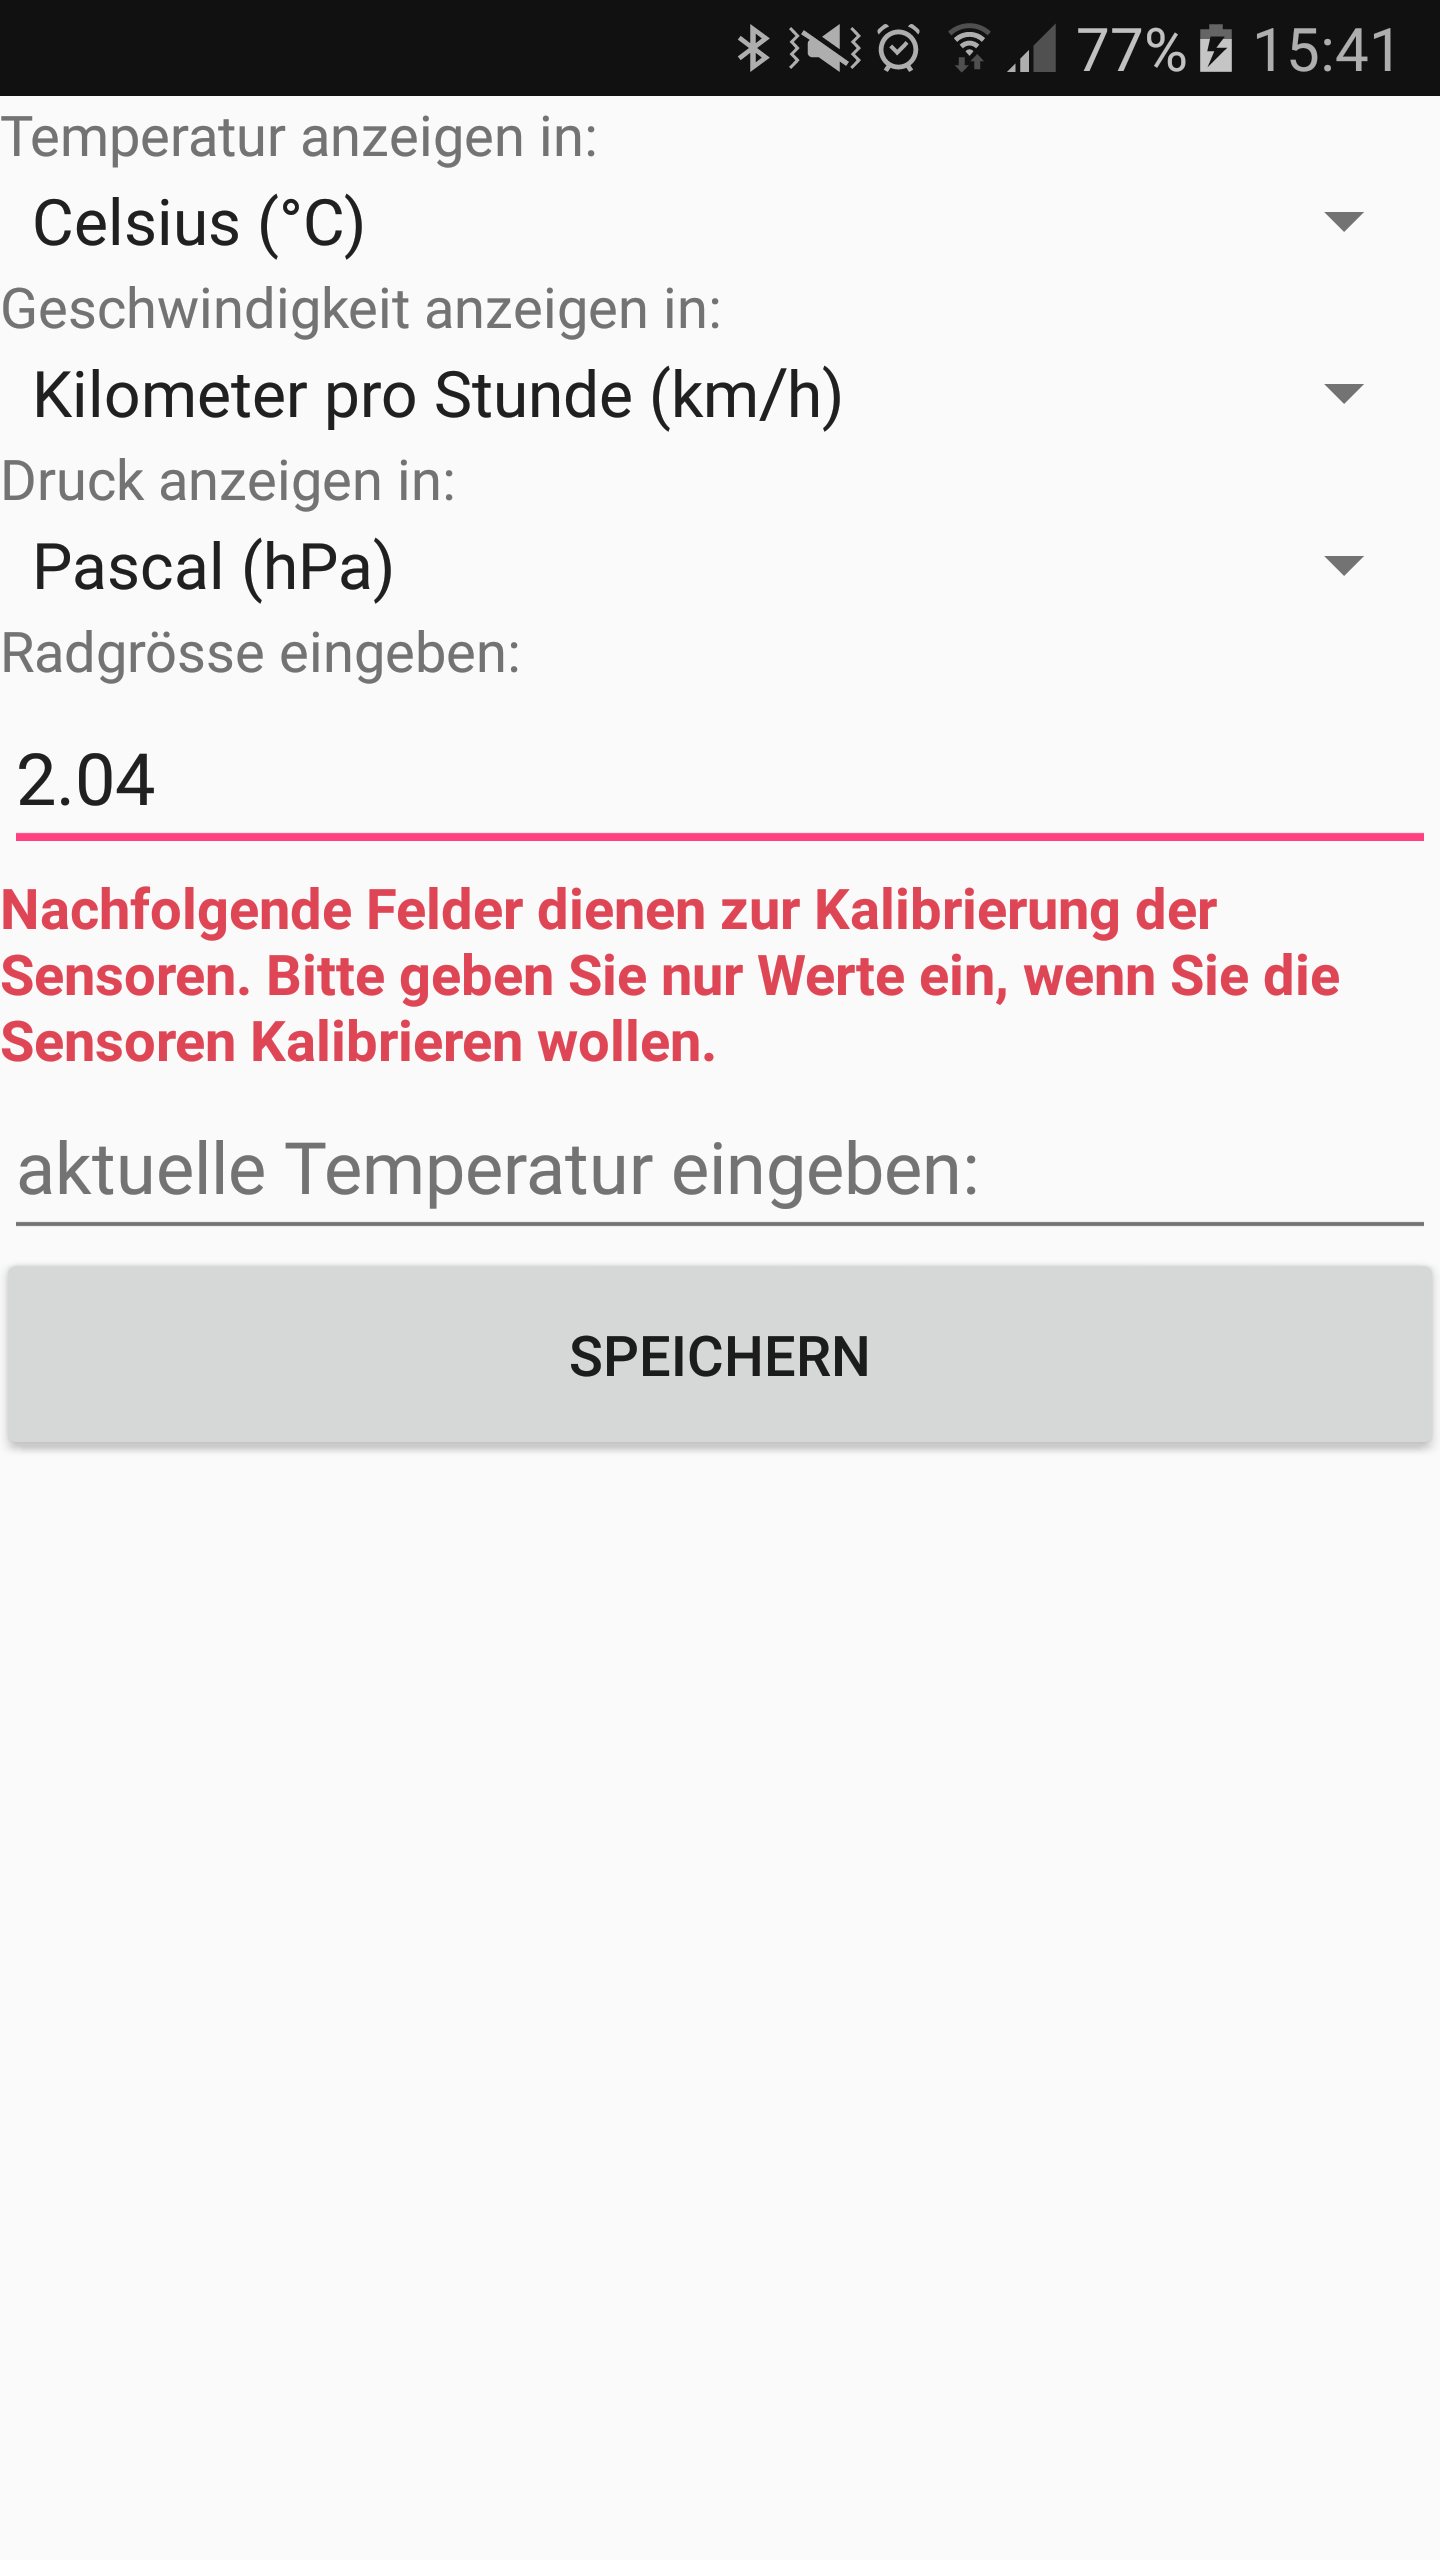
\includegraphics[width=0.5\textwidth]{4Resultate/imag/BLEEinheitenUndEinstellungenStart.png} 
    \caption{Einheiten und Einstellungen}
    \label{einheiten}
\end{figure}

Die Applikation stellt reiche Konfigurationsmöglichkeiten zur Verfügung (siehe Abbildung \ref{einheiten}. Zu jedem Sensor gehört eine Spinner. In den drei Spinner-Menüs stehen folgende Einheiten zur Verfügung:
 \todo{ Einheiten auflisten} 

Temperatur kalibriert werden kann. 
 
 
Radgrösse... 
  
Die vorgenommenen Einstellungen werden über den Button "Speichern" gesichert. Danach werden die eingelesenen Sensordaten in den ausgewählten Einheiten dargestellt.

\subsection{Paketverlust}

Es ist wichtig zu wissen, wie viele Pakete überhaupt bei der Applikation empfangen werden. Ein bekanntes Problem ist gem. Aussage von Dario, dass die meisten Smartphones nach einer gewissen Zeit die Bluetooth Schnittstelle nicht mehr die ganze Zeit eingeschalten lassen, sondern nur noch ca. 80\thinspace\% der Zeit die Bluetooth Schnittstelle betreiben. Das bedeutet, dass der Verlust von BLE-Paketen sehr wahrscheinlich ist. Die nachfolgende Tabelle zeigt den Paketverlust bei einer Geschwindigkeit von 20 km/h.

\todo{tabelle einfügen}




Ein Paketverlust 10\thinspace\% bis 20\thinspace\% war nach Aussage von Dario zu erwarten, da die meisten Smartphones die Bluetooth Schnittstelle nach einer gewissen Zeit nicht mehr die ganze Zeit betreiben. Der Betrieb der Bluetooth Schnittstelle wird reduziert, damit Energie gespart werden kann. 


\subsection{Korrektheit der Daten}

Natürlich bringt es nicht die Daten nur zu empfangen, es musste auch überprüft werden, ob die richtigen Daten empfangen wurden. Die Daten welche mit der Applikation empfangen wurden entsprechen exakt den Daten, welche der Sniffer empfangen hat. Somit kann garantiert werden, dass keine Informationen verloren gehen oder falsch interpretiert werden. Unvollständige Daten oder falsche Daten könnten in Anzeigefehlern oder gar dem Absturz der Applikation führen.

\todo{fertig schreiben}

\todo{Video zeiger (auf CD)}







\chapter{Diskussion}

Am Ende der Arbeit steht ein lauffähiger Prototyp eines Bicycle Computers zur Verfügung. Die Leistungsgewinnung ist um xxx \todo{Faktor} optimiert, der Aufbau minimiert und auf eine Leiterplatte gebracht, das Energy Management auf die Fahrgeschwindigkeit von 10 km/h optimiert sowie neu werden auch Sensordaten an die benutzerfreundliche Android-Applikation gesendet.

Der Prototyp ist so entwickelt, dass zukünftige Teams den Code schnell verstehen, die Leiterplatte leicht aufteilen und weiterentwickeln können und die modulare Android-Applikation ist nach Belieben ausbaubar.

Die Minimalanforderungen der definierten Aufgabenstellung wurden alle erreicht. Folgende optionale Aufgaben sind ebenfalls eingebettet worden: \todo{optionale Aufagaben auflisten}.

Als mögliche Weiterentwicklungen stehen insbesondere Energieverbrauchsoptimierungen an erster Stelle. Das Ziel ist, dass bis zur Präsentation des Bicycle Computer an der Nacht der Technik, die Sensoren mit weniger Energie ausgelesen werden, sodass die Versorgungsspannung bei Geschwindigkeiten unter 40 km/h nicht abstellt. Interessant ist die Auswirkung des Connected Modes bei höherer Geschwindigkeit. Bei tiefer ist der Verbindungsaufbau nicht realistisch. Doch bei höheren Geschwindigkeiten könnte über den Connected Mode sicher Daten versendet werden.

Die entwickelte Leiterplatte kann für Schülerinnen und Schüler zum Experimentieren mit BLE verwendet werden. Bewusst wurden viele Testpunkte und ein Stecker für das Abgreifen der Signale implementiert. Montagelöcher für eine Befestigung sind vorhanden und Steckplätze für die Kondensatoren gewähren einen flexiblen Einsatz der Kondensatoren. Das TI-SensorTag zusammen mit dem EM8500 eignen sich gut zum Kennenlernen des Energy Managements. 

Für die Aufführung des fertigen Produkts ist ein Gehäuse in Planung. Dieses wird an der Verstrebung Richtung Sattel. Die Distanz zum Rad, kann flexibel eingestellt werden, sodass der Prototyp sich nicht auf ein Fahrradmodell limitiert. Zum Endprodukt zählt auch eine professionelle Montage der Doppelmagnete an den Speichen. Als Letztes wird der Hohlraum zwischen der Leiterplatte und dem TI-SensorTag durch zwei Verstrebungen verstärkt, damit das Gerät Bodenschläge aushält. Das Endprodukt ist somit ein voll anwendungsfähiger Bicycle Computer. 

Auf das Produkt sind wir Stolz. Dies nicht zu Letzt, da die Umsetzung nicht ganz einfach war. Der EM8500-Chip ist ein neues Produkt und verhält sich teilweise nicht stabil. Konkret musste Manuel König acht EM8500-Chips auf die Leiterplatten anlöten, weil immer wieder einer ausstieg. Das heisst, entweder konnte die Kommunikation über SPI nicht mehr stattfinden, Slave-Address-Error, oder V_SUP startete trotz grosser Energie am Eingang nicht. Da der Chip nicht zuverlässig funktionierte, war es in der Entwicklung schwierig zu unterscheiden, ob in der Harversterschaltung ein Fehler auftrat oder der Chip einen Defekt aufwies. Zu oft suchten wir den Fehler in der Hardware und nicht im Chip. Die zweite Herausforderung ist die Benutzung des TI-SensorTags ohne RTOS. Diese rudimentäre Programmierung machte Spass. Mit Hilfe des Know-Hows am InES konnten die Probleme längerfristig gelöst werden. Da es Pionierarbeit ist, ging die Entwicklung des Codes nicht so schnell wie gewünscht vorwärts. Sinnvoll ist z.B. bei mehr Energie per SPI das Status Register des EM8500 auszulesen. In diesen 8 Bits steht der Zustand des Energyzustands der Speicher und welche Schwellwerte überschritten sind. 

Abschliessend möchten wir sagen, dass die Unterstützung bei der Bachelorarbeit sowohl von Prof. Dr. Meli wie auch von Research-Assistent Dario Dündar sehr gut war. Die Probleme, die auf uns zukamen, waren viel grösser als erwartet. Da wir es super im Team hatten, ergänzten uns auf eine gute Art und Weise. Die Freude blieb trotz teilweisem unerklärlichem, technischen Verhalten nie aus. Durch diese Arbeit haben wir sehr viel gelernt und freuen uns, zukünftig als Ingenieurin und als Ingenieur zu arbeiten.




\chapter{Verzeichnisse}




\renewcommand{\bibsection}{\section{\refname}}  % add a number to the bibl section
\makeatletter
%\renewcommand*\bib@heading{ \section{\refname}}
\makeatother


\bibliography{BibTex/references}



\section{Glossar und Abkürzungen}\label{glossar}

\textbf{Clock Domain}\\
Ein Bereich der Hardware, der mit demselben Takt läuft.

\textbf{Power Domain}\\
Basiert auf der Fähigkeit eines Prozessor Speisungsgebiete zur Verfügung zu stellen. Der Prozessor teilt seine Funktionalitäten in Gebiete ein, die separat ein- und ausgeschalten werden können.

\textbf{MPP}\\
Maximum Power Point (MPP) bezeichnet in einer Leistungskurve den höchsten Punkt, also das Leistungsmaxiumum.

\textbf{MPPT}\\
Versucht ein System, einen Input stets auf das Leistungsmaximum zu regeln, spricht man von Maximum Power Point Tracking. Tracking steht für Einfangen.

\textbf{MPPT-Ratio}\\
Bezeichnet die Auswertung des MPP auf Spannungsachse. Liegt das Leistungmaximum beim Kurzschluss, so ist die MPPT-Ratio bei 0 \%, liegt sie bei Leerlauf, dann liegt die MPPT-Ratio bei 100 \%. Üblicherweise liegt die MPPT-Ratio dazwischen.

\textbf{State Machine}
Heisst korrekt Finite State Machine und bezeichnet eine Konzept, bei dem aufgrund einer Kombination von Eingangssignalen, sich das System in einem bestimmten Zustand befindet. In jedem Zustand sind nur gewisse Inputs zulässig, ansonsten verbleibt das System in diesem Zustand. Folgt ein korrekter Input, wechselt das System in den entsprechenden Zustand. 



\textbf{UML}\\
Die Unified Modeling Language (UML) ist ein Quasistandard, wie Prozesse abgebildet werden können. Die Sprache definiert Formen, aufgrund deren man weiss, ob es sich um eine Initialiserung, eine Entscheidung oder um eine Verarbeitung, etc. handelt.


\section{Abbildungsverzeichnis}


\section{Tabellenverzeichnis}



%\addcontentsline{toc}{chapter}{Anhang}
\cftaddtitleline{toc}{chapter}{Anhang}{}
\pagenumbering{Roman}
\appendix


\chapter{Ausschreibung Bachelorarbeit}

\begin{figure}[h]
    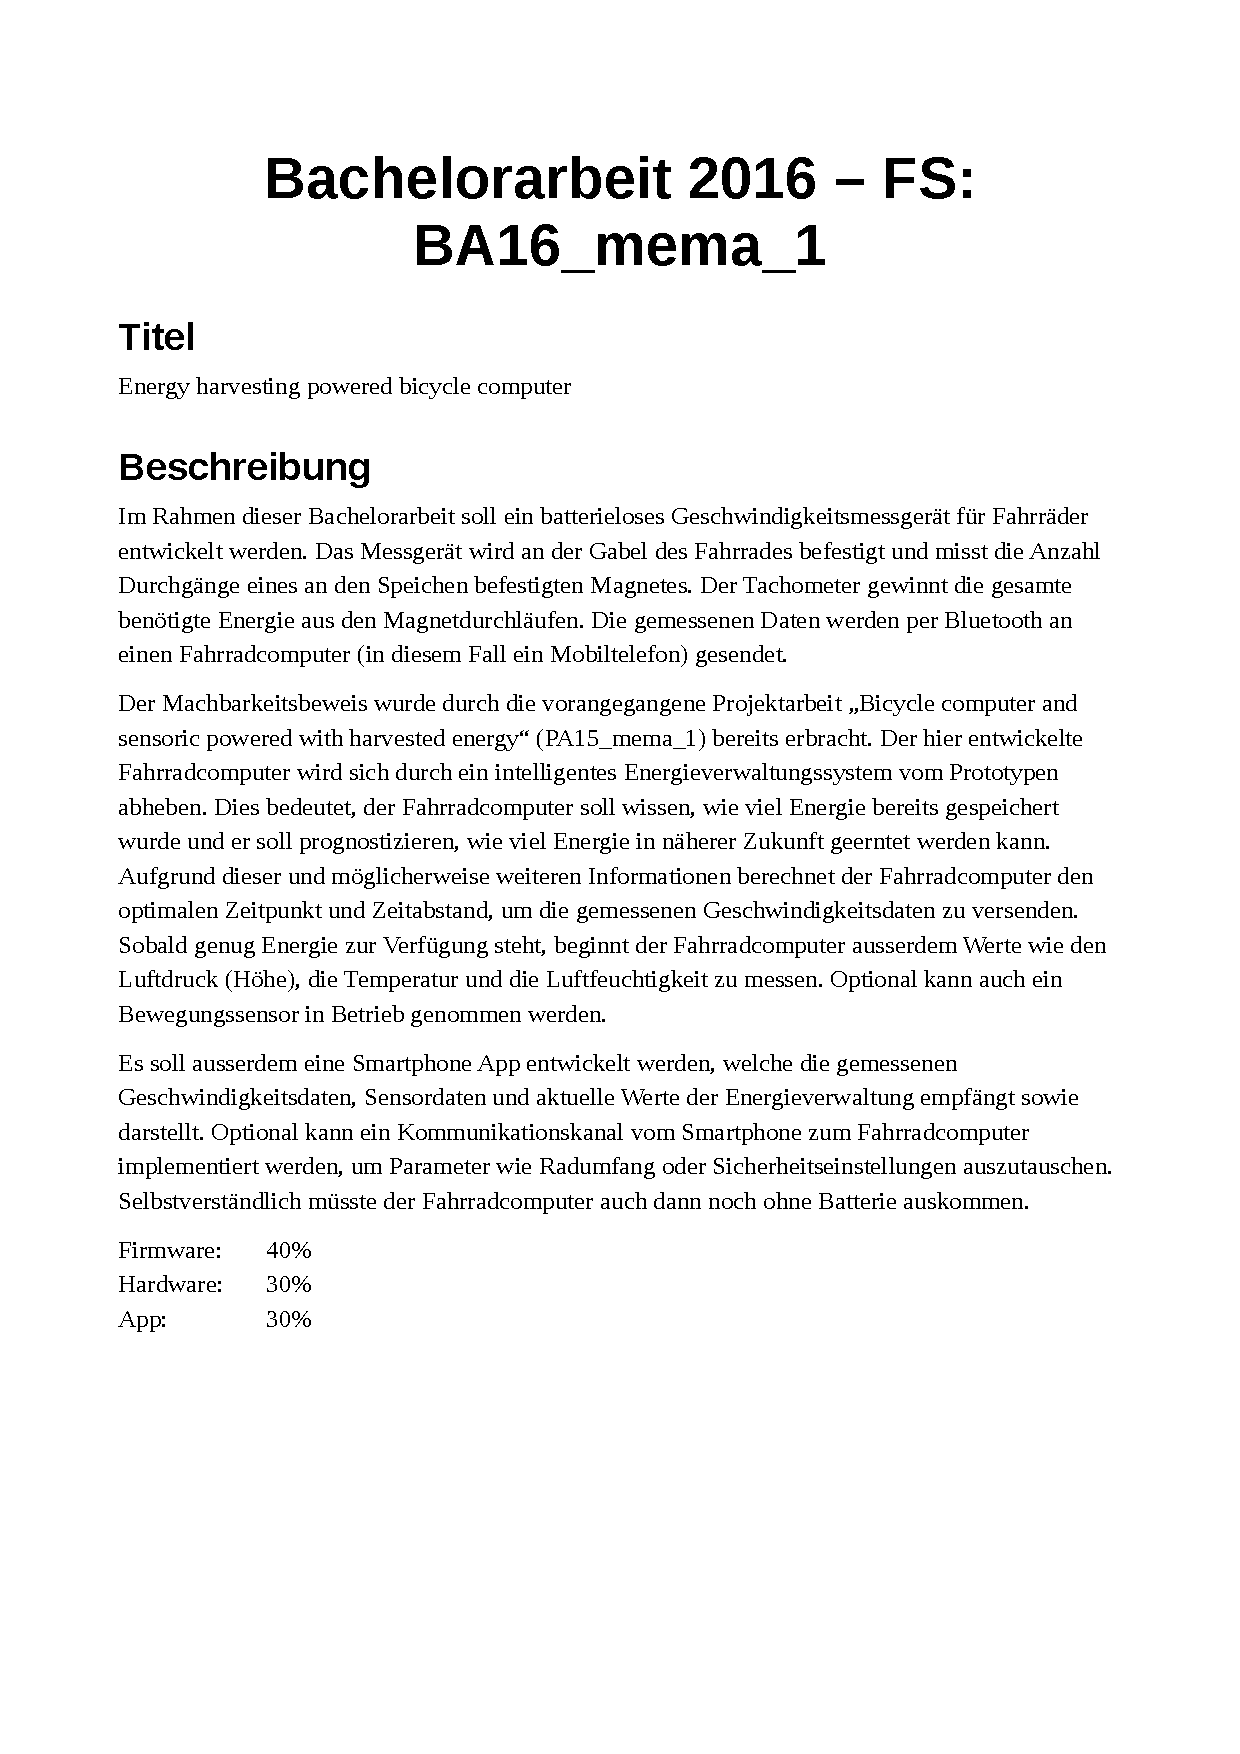
\includegraphics [width=0.8\textwidth] {7Anhang/docs/Ausschreibung.pdf} 
     \caption{Offizielle Ausschreibung der Arbeit}\label{Ausschreibung} 
\end{figure}



\chapter{Blockdiagramm EM8500}\label{anhang_em8500} 
\begin{figure}[h]
    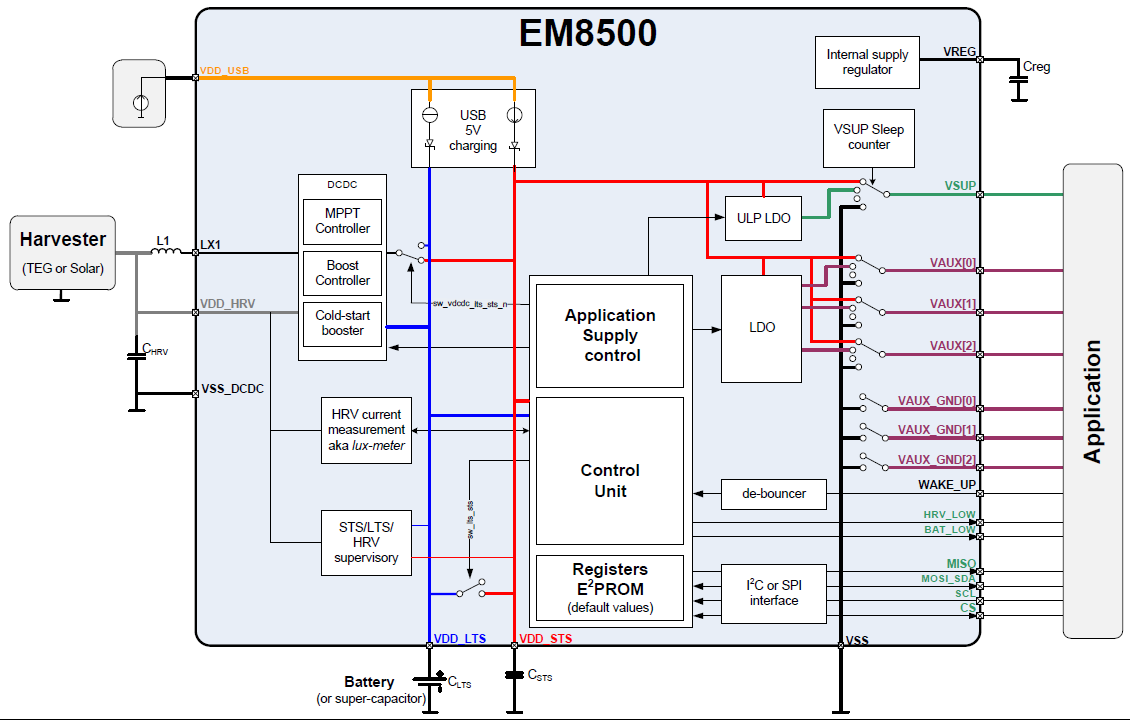
\includegraphics [width=1\textwidth]{7Anhang/imag/blockdiagrammEm8500.png} 
     \caption{Blockschema Sensortag}
\end{figure}



\chapter{Funktionsblöcke des TI-SensorTags}\label{anhang_sensortag} 

% hight

\begin{figure}[h]
    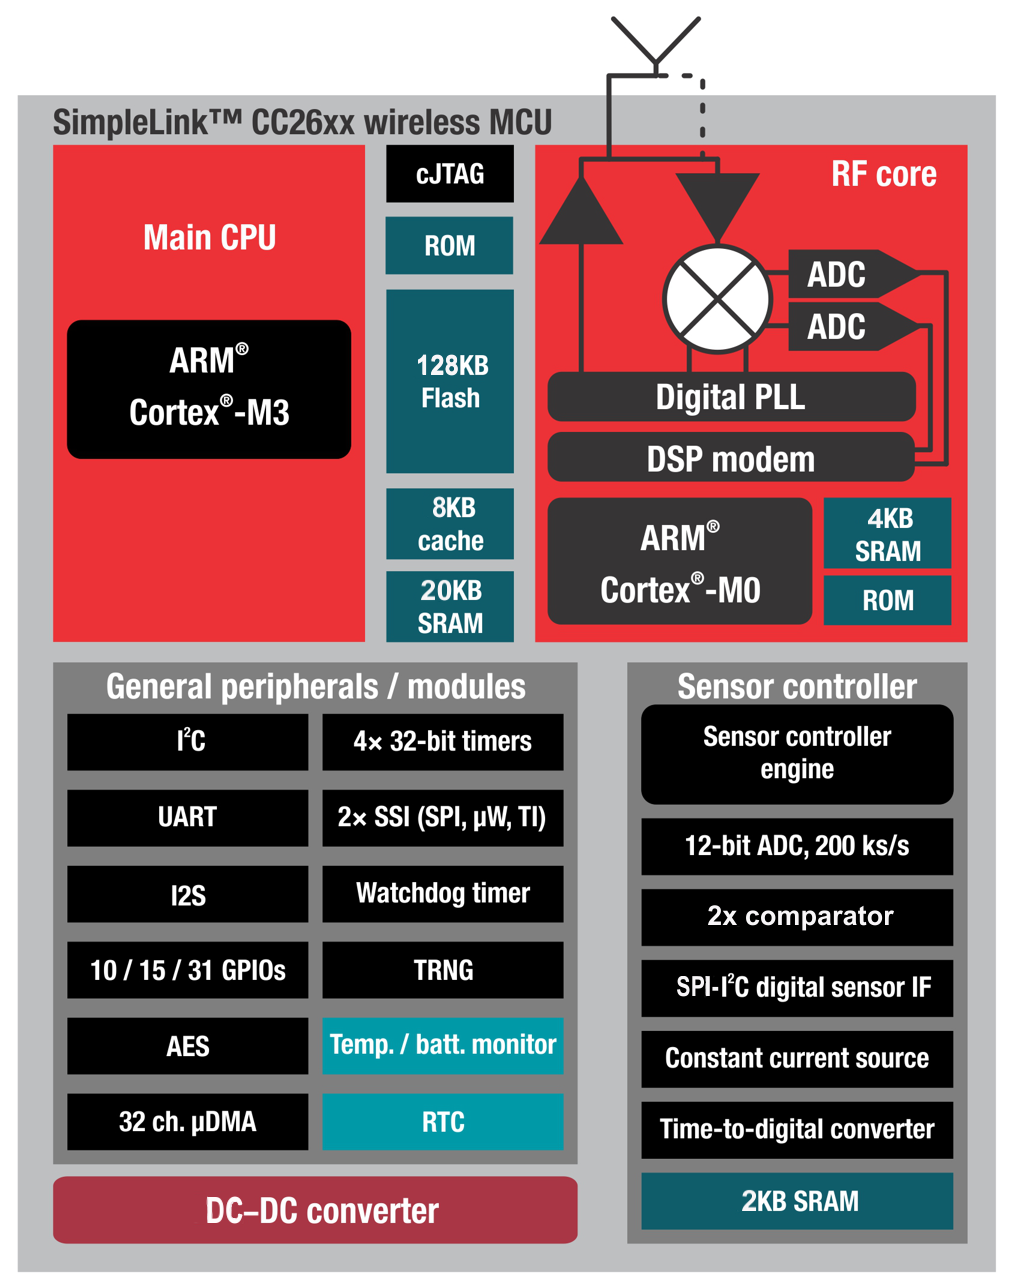
\includegraphics [width=0.7\textwidth]{7Anhang/imag/CC26xx_Block_Diagram.png} 
     \caption{Blockschema TI-SensorTag aus \cite{Sensortag_Datasheet}, S.3}
\end{figure}


\chapter{Supply System beim TI-SensorTag}
\label{anhang_sensortag_supply} 


\begin{figure}[h]
    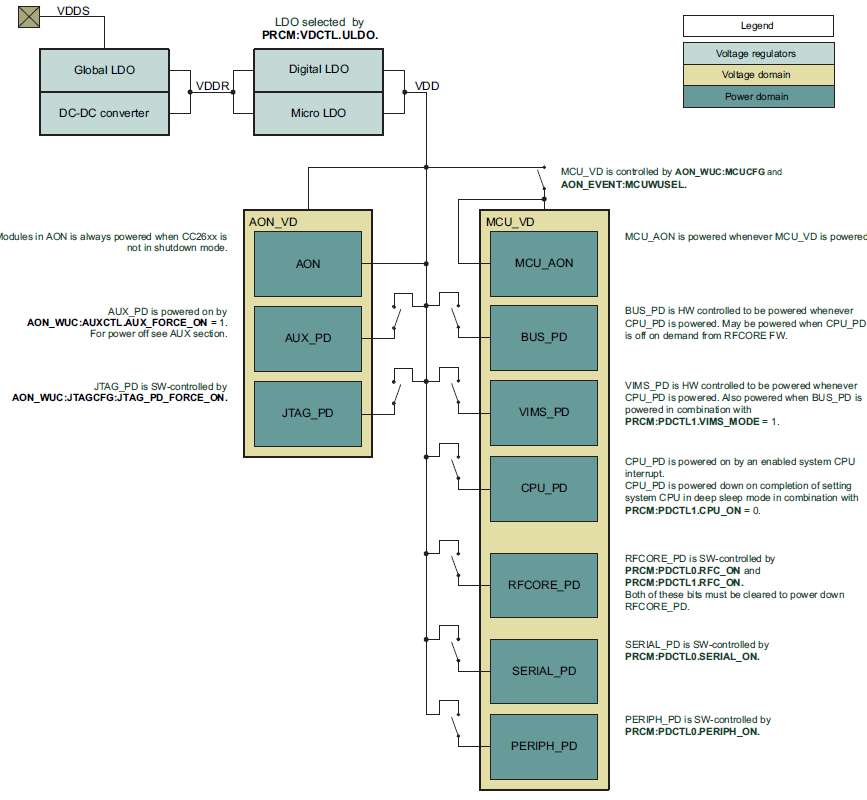
\includegraphics [width=0.7\textwidth]{7Anhang/imag/powerdomain_1.png} 
    \caption{Abbildung aus \cite{Sensortag_Manual}, S. 416}
    \label{a_supply}
\end{figure}

\chapter{Digital Power Partitioning beim TI-SensorTag}\label{anhang_sensortag_PowerDomain} 

% hight

\begin{figure}[h]
    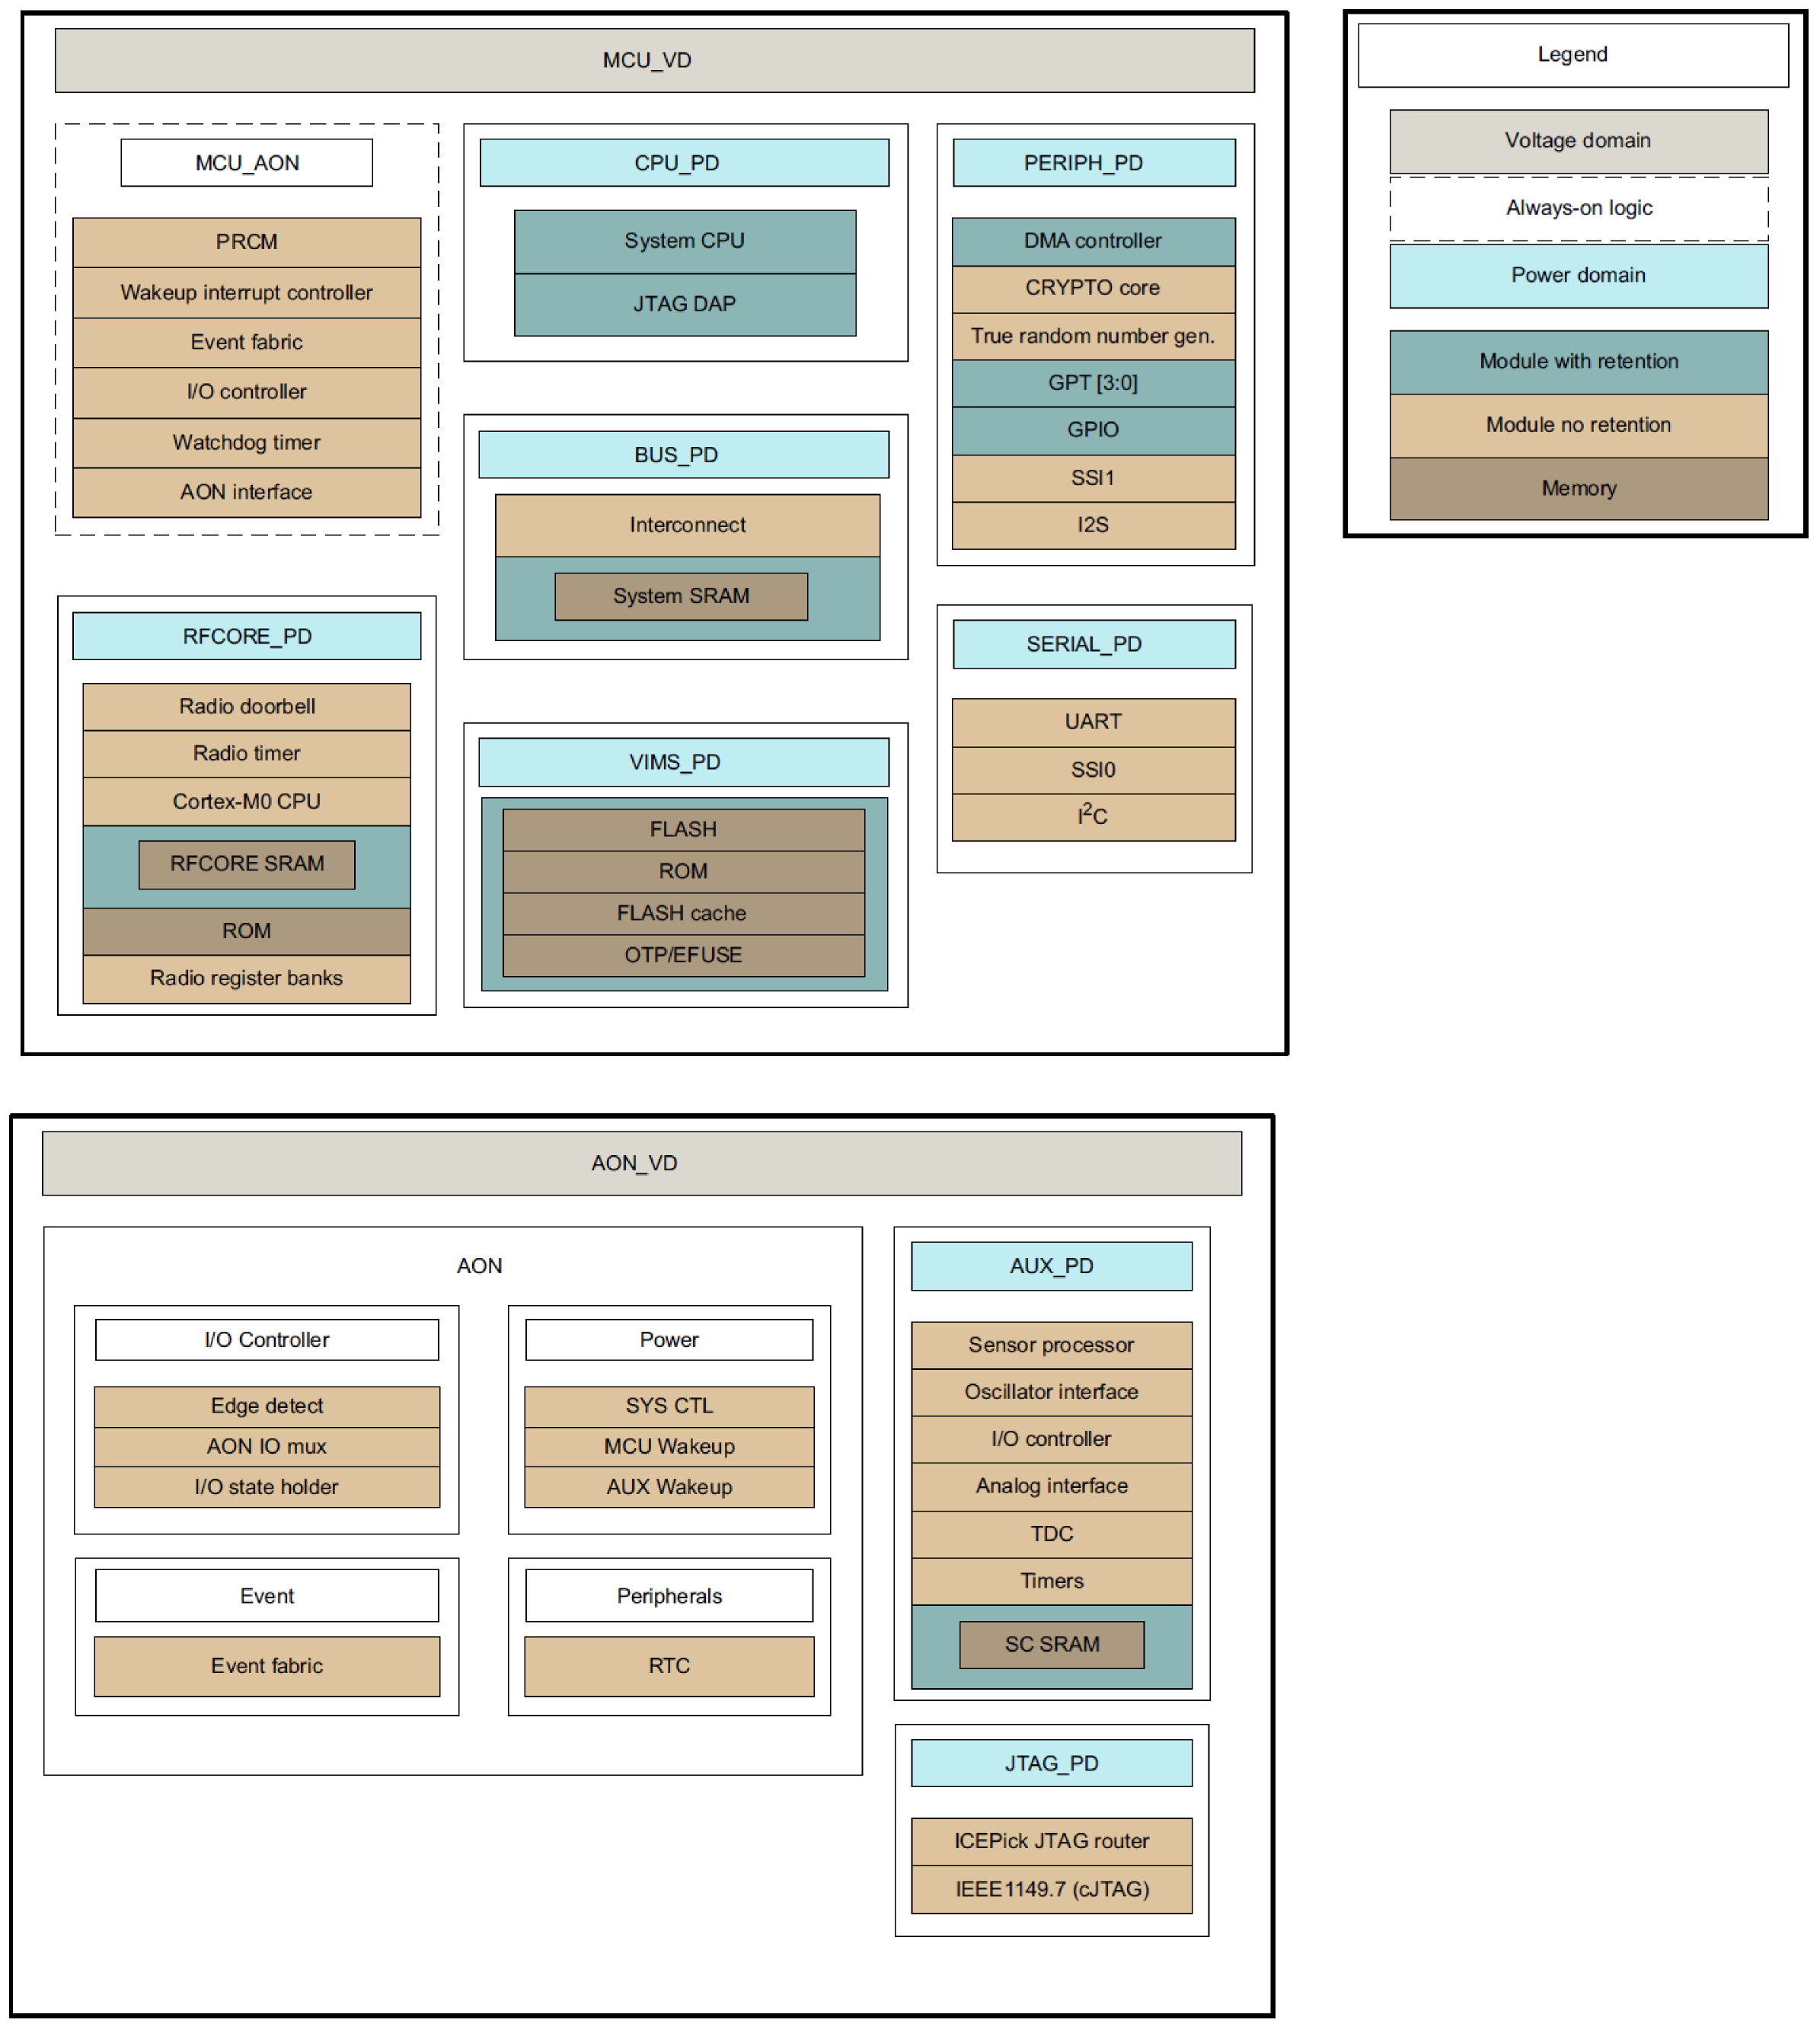
\includegraphics [width=0.7\textwidth]{7Anhang/imag/powerDomain_2.png} 
     \caption{Abbildung aus \cite{Sensortag_Manual}, S. 418}
     \label{a_powerdomain}
\end{figure}

\chapter{Messaufbau}
\label{messaufbau}
Problematisch war, dass die Messresultate mit dem Fahrrad nicht reproduzierbar waren, daher wurde eine Radimitation erarbeitet. Herr Erich Ruff hat einen Aubau entwickelt, welcher über einen Elektromotor angetrieben wurde, damit konnte die Geschwindigkeit relativ konstant gehalten werden. Die Toleranz der Geschwindigkeit lag bei +/- 1 km/h, was eine grosse Verbesserung gegenüber der bisherigen Vorgehensweise war.
Die Radimitation bestand aus nur einer Speiche, welche nur eine einfache Alustange war. An dieser Alustange waren mehrere Löcher zur Befestigung des Topfmagneten vorhanden.


\begin{figure}[ht]
    \includegraphics [width=1\textwidth]{7Anhang/imag/Messaufbau}
	\caption{Messaufbau während der Inbetriebnahme des Prototypen}
	\label{messaufbau_anhang}
\end{figure}

Der Radimitation ist ein Tachometer angehängt, der die aktuelle Geschwindigkeit anzeigt. Der Tachometer ist vom Hersteller SIGMA Sport, die genaue Bezeichnung Lautet SIGMA SPORT BASELINE 500. Dieser Tachometer wurde im Jahr 1999 hergestellt, funtioniert jedoch nach wie vor einwandfrei.

Im Verlauf der Entwicklung wurde entschieden, dass zwei Magnete im Abstand von 180 Grad angebracht werden. Diese Entscheidung wurde getroffen, um die Energiegewinnung zu maximieren, es wurde jedoch ebenfalls entschieden, dass nicht mehr als zwei Magnete montiert werden sollen. Das Erscheinungbild des Fahrrads würde damit sehr beeinträchtigt und die Bremswirkung würde mit vielen Magneten sicherlich zum Tragen kommen.

Alle Messungen wurden mit einem Radumfang von 2.04 m ausgeführt, der Magnet befand sich 25 cm vom Zentrum der Radsimulation entfernt. Den Einfluss des Abstands kann aus dem Messprotokoll vom 06. Mai 2016 entnommen werden.

\chapter{Übersicht Messprotokolle}
\label{uebersicht_messprotokolle}

\subsubsection*{Übersicht Messprotokolle  }
\label{tabelle_uebersicht_messprotokolle}
\begin{tabbing}
       Messdatum	   	\quad\= Messobjekt    		\quad\= Name des PDF     \\[0.8ex]
	   26. Februar 2016 \> Harvesterausgang Elko 	\> Messprotokoll\_Kondensator\_Ausgang\_Harvesterschaltung.pdf\\
	   14. März 2016 	\> Spule 					\> Messprotokoll\_Optimierung\_Spule.pdf\\
	   14. März 2016 	\> Gleichrichter 			\> Messprotokoll\_Optimierung\_Gleichrichter\_1.pdf\\
	   14. März 2016 	\> Gleichrichter 			\> Messprotokoll\_Optimierung\_Gleichrichter\_2.pdf\\
	   14. März 2016 	\> Spannungsbegrenzung 		\> Messprotokoll\_Optimierung\_Limiter.pdf\\
	   19. März 2016 	\> Harvesterausgang 		\> Messprotokoll\_Leistungskennlinie\_Harvester\_versch\_Harvester.pdf\\
	   30. März 2016 	\> EM8500-Chip-Ausgang 		\> Messprotokoll\_Leistungskennlinie\_Harvester\_fliegender\_Aufbau.pdf\\
	   14. April 2016 	\> Spule und Magnete 		\> Messprotokoll\_Optimierung\_Spule\_versch\_Spulen\_und\_Magnete.pdf\\
	   14. April 2016 	\> Harvesterausgang 		\> Messprotokoll\_Leistungskennlinie\_Harvester\_Prototypenhardware.pdf\\
	   06. Mai 2016 	\> Harvesterausgang 		\> Messprotokoll\_Leistungskennlinie\_Position\_Magnet.pdf\\
	   16. Mai 2016 	\> Prototyp 				\> Messprotokoll\_Inbetriebnahme\_Prototyp.pdf\\
	   16. Mai 2016 	\> Harvesterausgang 		\> Messprotokoll\_Leistungskennlinie\_Harvesterausgang\_Prototyp.pdf\\
       18. Mai 2016 	\> EM8500-Chip-Ausgang 		\> Messprotokoll\_Energiemessung\_EM-Chip\_Inbetriebnahme.pdf\\	   
	   19. Mai 2016 	\> Prototyp 				\> Messprotokoll\_Inbetriebnahme\_Prototyp\_Energiemanagment.pdf\\
	   21. Mai 2016 	\> Harvesterausgang Elko 	\> Messprotokoll\_Harvesterausgang\_Elko.pdf\\
	   21. Mai 2016 	\> Harvesterausgang 		\> Messprotokoll\_Leistungskennlinie\_Harvesterausgang\_endgültige\_Hardware.pdf\\
	   22. Mai 2016 	\> BLE-Kommunikation 		\> Messprotokoll\_BLE\_Kommunikation\_Paketverlust.pdf\\ %vorhanden
	   28. Mai 2016 	\> EM8500-Chip-Ausgang 		\> Messprotokoll\_Energiemessung\_EM-Ausgang\_endgültige\_Hardware.pdf\\ %vorhanden
	   03. Juni 2016 	\> TI-SensorTag 			\> Messprotokoll\_Energieverbrauch\_Sensortag.pdf\\
\end{tabbing}  



\end{document}


